\documentclass[12pt,a4paper,twoside]{book}
% Language setup for Greek and English
\usepackage[english,greek]{babel}
\usepackage[utf8]{inputenc}
\usepackage[T1,LGR]{fontenc}
% Font setup
\usepackage{fontspec}
\setmainfont{Linux Libertine O}[Scale=0.9]
\setsansfont{Linux Biolinum}[Scale=0.9]
\setmonofont{DejaVu Sans Mono}[Scale=0.9]
% Other necessary packages
\usepackage{enumitem}
\usepackage{graphicx}
\usepackage{amsmath}
\usepackage{makeidx}
\usepackage{multicol}
\usepackage{multirow}
\usepackage{hanging}
\usepackage{adjustbox}
\usepackage{amssymb}
\usepackage{stackengine}
\usepackage{ifthen}
\usepackage{array}
\usepackage{tcolorbox}
\tcbuselibrary{skins,breakable}
\usepackage{minted}
\usepackage{listings}
\usepackage{parskip}
\usepackage{float}
\usepackage{subcaption}
\usepackage{xcolor}
\usepackage{cancel}
\usepackage{pdfpages}
\usepackage{titlesec}
% Page & text layout
\usepackage{geometry}
\geometry{
   a4paper,
   top=2.5cm,
   bottom=2.5cm,
   left=2.5cm,
   right=2.5cm
}
% Headers & footers
\usepackage{fancyhdr}
\pagestyle{fancyplain}
\fancyhf{} % Clear all header/footer fields

% Define plain style for chapter pages and TOC
\fancypagestyle{plain}{%
    \fancyhf{} % Clear all header/footer fields
    \renewcommand{\headrulewidth}{0pt} % Remove header rule
    \renewcommand{\footrulewidth}{0pt} % Remove footer rule
}

% Define TOC style with specific headers
\fancypagestyle{tocstyle}{%
    \fancyhf{} % Clear all header/footer fields
    \fancyhead[LE]{\thepage}
    \fancyhead[CE]{\leftmark}
    \fancyhead[CO]{\rightmark}
    \fancyhead[RO]{\thepage}
    \renewcommand{\headrulewidth}{0pt}
}

% Redefine \tableofcontents to use tocstyle
\let\oldtableofcontents\tableofcontents
\renewcommand{\tableofcontents}{%
    \clearpage
    % First page of TOC should be empty
    \thispagestyle{empty}
    \pagestyle{tocstyle}
    \oldtableofcontents % chktex 1
    \clearpage
    \pagestyle{fancy}
    % Regular pages header settings
    \fancyhead[LE]{\thepage} % Left header on Even pages: Shows page number
    \fancyhead[CE]{\leftmark} % Center header on Even pages: Shows chapter name (stored in \leftmark)
    \fancyhead[RE]{ΚΕΦ. \thechapter} % Right header on Even pages: Shows "ΚΕΦ." followed by chapter number % chktex 12

    \fancyhead[LO]{\thesection} % Left header on Odd pages: Shows current section number
    \fancyhead[CO]{\rightmark} % Center header on Odd pages: Shows section name (stored in \rightmark)
    \fancyhead[RO]{\thepage} % Right header on Odd pages: Shows page number

    \renewcommand{\headrulewidth}{0.4pt} % Sets thickness of the horizontal line below the header

    % Redefine chapter mark to remove "Chapter" prefix
    \renewcommand{\chaptermark}[1]{\markboth{##1}{}}
    % Redefine section mark to use section title only
    \renewcommand{\sectionmark}[1]{\markright{##1}}
}

% Make table of contents use plain style
\addtocontents{toc}{\protect\thispagestyle{plain}}

% Hyperlinks
\usepackage{hyperref}
\usepackage{bookmark}                                       % Add this line to fix the hyperref warnings
\hypersetup{
    colorlinks=true,
    linkcolor=blue,
    citecolor=blue,
    filecolor=blue,
    urlcolor=cyan,
    unicode,
    pdftitle={Pet-à-Vet},
    pdfsubject={Αναφορά Project},
    pdfborderstyle={/S/U/W 1},                              % Underline links
}
\usepackage{tikz}
\usetikzlibrary{positioning, shapes.geometric, arrows.meta}
\usepackage{pgfplots}
\pgfplotsset{compat=1.18}
\usetikzlibrary{calc,arrows.meta,positioning}

\definecolor{customRed}{HTML}{FF5F5A}                       % using hexadecimal
\definecolor{customYellow}{HTML}{FFBE2E}                    % using hexadecimal
\definecolor{customGreen}{HTML}{2ACA44}                     % using hexadecimal
\definecolor{customPurple}{HTML}{C477DB}                    % using hexadecimal
\definecolor{customBlue}{HTML}{052538}                      % using hexadecimal
\definecolor{customLightBlue}{HTML}{60ADEC}                 % using hexadecimal
\definecolor{customGray}{HTML}{A0A0A0}                      % using hexadecimal
\definecolor{customBlack}{HTML}{000000}                     % using hexadecimal

% Define a lighter gray for background and darker colors for text
\definecolor{customBgGray}{HTML}{E0E0E0}         % Light gray background
\definecolor{customCodeRed}{HTML}{C92A2A}        % Darker red
\definecolor{customCodeYellow}{HTML}{E67700}     % Darker yellow/orange
\definecolor{customCodeGreen}{HTML}{087F23}      % Darker green
\definecolor{customCodePurple}{HTML}{7B1FA2}     % Darker purple
\definecolor{customCodeBlue}{HTML}{1976D2}       % Darker blue
\definecolor{customCodeBlack}{HTML}{1A1A1A}      % Lighter black

\lstdefinestyle{myPythonStyle}{
    language=Python,                                            % Set the language to Python
    backgroundcolor=\color{customBgGray},                       % Background color
    basicstyle=\color{customCodeBlack}\ttfamily\footnotesize,   % Basic font style, size, and color
    keywordstyle=\color{customCodePurple}\bfseries,             % Style for general keywords
    keywordstyle=[2]\color{customCodeYellow}\bfseries,          % Style for specific keywords
    commentstyle=\color{customCodeGreen}\itshape,               % Style for comments
    stringstyle=\color{customCodeGreen},                        % Style for strings
    identifierstyle=\color{customCodeBlue},                     % Style for identifiers
    morekeywords={self, None, True, False, format, abs,
                as, pass, return, if, elif, else, for,
                range, while, try, except, with, lambda,
                yield, global, nonlocal, assert, del,
                raise, in, is, and, or, not},                   % Additional keywords
    morekeywords=[2]{os, graphviz, Digraph, collections,
                    deque, math, tabulate},                     % Define 'import' and 'from' as additional keywords
    % procnamekeys={def,class},                                 % Highlight function and class names
    showstringspaces=false,                                     % Don't show spaces in strings
%
    breaklines=true,                                            % Automatically break long lines
    breakatwhitespace=false,                                    % Break lines at any character
    % prebreak=\textbackslash,                                  % Character for breaking lines
    postbreak={\space},                                         % Character for breaking lines
    breakautoindent=false,                                      % Indentation after line break
    breakindent=0pt,                                            % Indentation before line break
    resetmargins=true,                                          % Reset margins after line break
    keepspaces=true,                                            % Keep spaces in the code
    showspaces=false,                                           % Don't show spaces
    columns=flexible,                                           % Column format
%
    numbers=left,                                               % Line numbers on the left
    numberstyle=\small\color{customBgGray},                     % Style for line numbers
    % numwidth=4em,                                             % Width allocated for line numbers
    stepnumber=1,                                               % Step between line numbers
    numbersep=8pt,                                              % Distance of line numbers from code
    xleftmargin=1.5em,                                          % Match the numwidth
    tabsize=4,                                                  % Size of a tab
    captionpos=t,                                               % Position of the caption (t for top)
    firstnumber=auto,                                           % Continue line numbering from previous listing
    aboveskip=0em,                                              % Remove external spacing
    belowskip=0em,                                              % Remove external spacing
    frame=none,                                                 % Add top and bottom rules only
    framerule=0pt,                                              % Make the rules invisible
    rulecolor=\color{customBgGray},                             % Color of the frame (if enabled)
    framesep=2pt,                                               % Add internal padding
    % framexleftmargin=1em,                                     % Add internal left margin
    % framexrightmargin=1em,                                    % Add internal right margin
    escapeinside={\(*@}{@*\)},                                  % For escaping characters
    morecomment=[l]{\#},                                        % Define comment style
    morestring=[b]',                                            % Define string style with single quotes
    morestring=[b]",                                            % Define string style with double quotes % chktex 18
    literate={
        {``}{{\textquotedbleft}}2
        {''}{{\textquotedbright}}2
        {`}{{\textquoteleft}}1
        {'}{{\textquoteright}}1
        {_}{{\_}}1
    },
}

\lstdefinestyle{myCStyle}{
    language=C,
    backgroundcolor=\color{customBgGray},                       % Background color
    basicstyle=\color{customCodeBlack}\ttfamily\footnotesize,   % Basic font style
    keywordstyle=\color{customCodePurple}\bfseries,            % Style for keywords
    keywordstyle=[2]\color{customCodeYellow}\bfseries,         % Style for additional keywords
    commentstyle=\color{customCodeGreen}\itshape,              % Style for comments
    stringstyle=\color{customCodeGreen},                       % Style for strings
    identifierstyle=\color{customCodeBlue},                    % Style for identifiers
    morekeywords={void, int, char, float, double, long, short, signed, unsigned,
                  const, static, extern, volatile, register, auto, struct, union,
                  typedef, enum, sizeof, break, continue, goto, return, if, else,
                  switch, case, default, for, while, do, pid_t, sem_t},
    morekeywords=[2]{stdio.h, stdlib.h, string.h, math.h, time.h, ctype.h,
                     unistd.h, semaphore.h, sys/mman.h, sys/wait.h, fcntl.h,
                     printf, fprintf, perror, exit, malloc, free, fork, waitpid,
                     mmap, munmap, sem_init, sem_wait, sem_post, sem_destroy,
                     sleep, rand, srand, atoi, time, MAP_SHARED, MAP_ANONYMOUS,
                     PROT_READ, PROT_WRITE, MAP_FAILED, EXIT_SUCCESS, EXIT_FAILURE},
    showstringspaces=false,
    frame=none,
    rulecolor=\color{customBgGray},
    breaklines=true,                % Break long lines
    breakatwhitespace=false,        % Break at any character
    postbreak={\space},             % Character after break
    breakautoindent=false,          % No indentation after break
    breakindent=0pt,                % No indent before break
    resetmargins=true,              % Reset margins after break
    keepspaces=true,                % Preserve spaces
    showspaces=false,               % Don't show spaces
    columns=flexible,               % Column format
    numbers=left,
    numberstyle=\small\color{customBgGray},
    stepnumber=1,
    numbersep=8pt,
    xleftmargin=1.5em,
    tabsize=4,
    captionpos=t,
    firstnumber=auto,
    aboveskip=0em,
    belowskip=0em,
    framesep=2pt,
    escapeinside={\(*@}{@*\)},
    morecomment=[l]{//},
    morecomment=[s]{/*}{*/},
    morestring=[b]", % chktex 18
    morestring=[b]',
    literate={
        {``}{{\textquotedbleft}}2
        {''}{{\textquotedbright}}2
        {`}{{\textquoteleft}}1
        {'}{{\textquoteright}}1
        {_}{{\_}}1
    },
}

\lstdefinestyle{myBashStyle}{
    language=bash,
    backgroundcolor=\color{customBgGray},                       % Background color
    basicstyle=\color{customCodeBlack}\ttfamily\footnotesize,   % Basic font style
    keywordstyle=\color{customCodePurple}\bfseries,            % Style for keywords
    keywordstyle=[2]\color{customCodeYellow}\bfseries,         % Style for additional keywords
    commentstyle=\color{customCodeGreen}\itshape,              % Style for comments
    stringstyle=\color{customCodeGreen},                       % Style for strings
    identifierstyle=\color{customCodeBlue},                    % Style for identifiers
    alsoletter={0123456789}                                    % Define numbers as letters
    morekeywords={if, then, else, elif, fi, for, while, do, done, in, case, esac, 
                  function, select, until, break, continue, return, exit, shift,
                  declare, local, readonly, export, set, unset},
    morekeywords=[2]{echo, read, cat, awk, grep, sed, cut, tr, sort, uniq, wc,
                     mkdir, rm, cp, mv, ls, cd, pwd, touch, chmod, chown, find,
                     test, source, alias, eval, exec, getopts, printf, wait,
                     STDIN, STDOUT, STDERR, IFS, PATH, BEGIN, END, NR, NF, 
                     tolower, concat, print},
    showstringspaces=false,
    frame=none,
    rulecolor=\color{customBgGray},
    breaklines=true,                % Break long lines
    breakatwhitespace=false,        % Break at any character
    postbreak={\space},             % Character after break
    breakautoindent=false,          % No indentation after break
    breakindent=0pt,                % No indent before break
    resetmargins=true,              % Reset margins after break
    keepspaces=true,                % Preserve spaces
    showspaces=false,               % Don't show spaces
    columns=flexible,               % Column format
    numbers=left,
    numberstyle=\small\color{customBgGray},
    stepnumber=1,
    numbersep=8pt,
    xleftmargin=1.5em,
    tabsize=4,
    captionpos=t,
    firstnumber=auto,
    aboveskip=0em,
    belowskip=0em,
    framesep=2pt,
    escapeinside={\(*@}{@*\)},
    morecomment=[l]{\#},
    morestring=[b]", % chktex 18
    morestring=[b]',
    literate={
        {``}{{\textquotedbleft}}2
        {''}{{\textquotedbright}}2
        {`}{{\textquoteleft}}1
        {'}{{\textquoteright}}1
        {_}{{\_}}1
    },
}

\tcbset{
    myCustomStyle/.style={
        enhanced,                       % Enable enhanced features
        breakable,                      % Allow the box to break across pages
        colback=customBlue,             % Background color
        colframe=customBgGray,              % Frame color
        listing only,                   % Use listings
%
        fonttitle=\bfseries,            % Title font style
        % frame=single,                 % Frame type
        % interior titled,              % Use regular titled interior
        interior style={
            top color=black!75,         % Title area background
            bottom color=black!75,      % Title area background
        },
        colbacktitle=black!75,          % Title background color
        coltitle=white,                 % Title color
        rounded corners,                % Rounded corners
        boxrule=1mm,                    % Frame thickness
        drop shadow southeast,          % Shadow effect
        lefttitle=0pt,                  % Remove left margin of title
        % left=1em,                     % Increase left margin for line numbers
        title={\hspace*{-1em}\textcolor{customRed}{● }\textcolor{customYellow}{● }\textcolor{customGreen}{●}\quad#1}, % Circles + Title
        attach title to upper={\vspace{2.3mm}}, % Adjust vertical spacing
%
        beforeafter skip=8pt,           % Space before and after the box
        breaklines=true,                % Allow the box to break across pages
        breakatwhitespace=false,        % Break lines at any character if necessary
        % sharp corners                 % Sharp corners for the title area
    }
}

% Custom commands for language switching
\newcommand{\en}[1]{\foreignlanguage{english}{#1}}
\newcommand{\gr}[1]{\foreignlanguage{greek}{#1}}
% Custom command for coloring
\newcommand{\blue}[1]{\textcolor{blue}{#1}}
% Index
\makeindex
% Set headheight to avoid fancyhdr warnings
\setlength{\headheight}{14.5pt}

% Adjust chapter spacing
\titleformat{\chapter}[display]
{\normalfont\huge\bfseries}{\chaptertitlename\ \thechapter}{15pt}{\Huge}
\titlespacing*{\chapter}{0pt}{-10pt}{20pt}

% Adjust section spacing
\titlespacing*{\section}{0pt}{10pt}{10pt}

% Adjust vertical space between paragraphs
\setlength{\parskip}{0.5em}

% Make figure placement less strict
\setcounter{topnumber}{2}
\setcounter{bottomnumber}{2}
\setcounter{totalnumber}{4}
\renewcommand{\topfraction}{0.85}
\renewcommand{\bottomfraction}{0.85}
\renewcommand{\textfraction}{0.15}
\renewcommand{\floatpagefraction}{0.7}

\begin{document}
% Start Arabic numbering from the beginning but hide numbers
\pagenumbering{arabic}
% Add this command to prevent blank pages
\let\cleardoublepage\clearpage

% Set main language to Greek
\selectlanguage{greek}

% Title page with hidden number
\begin{titlepage}
  \vspace*{5cm}
  \begin{center}
    
\includegraphics[width=0.3\textwidth]{Resources/Pet-a-vet-logo-transparent.png}\\
    % {\LARGE \textbf{\textit{Pet-à-Vet}}}\\ % chktex 8
    \vspace*{0.5cm}
    {\large Τεχνολογία Λογισμικού}
    \vspace*{5cm}
    \\
    \vspace*{1cm}
    \begin{tabular}{l l l}
      \large Αλέξανδρος Γιαννακόπουλος   & \large 1100520 & \large up1100520@ac.upatras.gr \\ % chktex 19
      \large Αριάδνη Σβωλοπούλου         & \large 1104806 & \large up1104806@ac.upatras.gr \\ % chktex 19
      \large Βασίλειος Μπίτζας           & \large 1083796 & \large up1083796@ac.upatras.gr \\
      \large Κωνσταντίνος Βασιλακόπουλος & \large 1090047 & \large up1090047@ac.upatras.gr \\
      \large Σάββας Δανιήλογλου          & \large 1084640 & \large up1084640@ac.upatras.gr
    \end{tabular}

    \vspace*{1cm}

    {\normalsize Τμήμα Μηχανικών Η/Υ \& Πληροφορικής}
    \\
    {\normalsize Πανεπιστήμιο Πατρών}
    \\
  \end{center}
  \thispagestyle{empty} % Suppress page number on the title page
\end{titlepage}

% % Add this command to prevent blank pages
% \let\cleardoublepage\clearpage
% \frontmatter
\tableofcontents
% \mainmatter % chktex 1

\printindex

\chapter{Project-description-v0.1}

\section{Περιγραφή Έργου}

Στο πλαίσιο του εργαστηρίου Τεχνολογίας Λογισμικού θα αναπτυχθεί μία ολοκληρωμένη ψηφιακή πλατφόρμα διαχείρισης κτηνιατρικών υπηρεσιών με την ονομασία Pet-à-Vet. Η πλατφόρμα στοχεύει στην εξυπηρέτηση πολλαπλών ομάδων χρηστών, όπως ιδιοκτήτες κατοικίδιων, κτηνιατρικές κλινικές, προσωπικό κλινικών και επαγγελματίες εκτροφείς. Το σύστημα θα προσφέρει ένα βασικό δωρεάν επίπεδο λειτουργιών και προηγμένες δυνατότητες μέσω συνδρομητικών πακέτων. % chktex 19

Η εφαρμογή θα διαθέτει ένα εξελιγμένο σύστημα διαχείρισης ραντεβού που θα επιτρέπει την online κράτηση με επιλογή κτηνιάτρου και ώρας επίσκεψης, ενώ παράλληλα θα παρέχει αυτοματοποιημένες υπενθυμίσεις μέσω email ή SMS. Οι ιδιοκτήτες θα μπορούν να φτιάξουν προφίλ στην εφαρμογή και να εισάγουν τα κατοικίδια τους. Για τους κτηνιάτρους, το σύστημα θα προσφέρει ολοκληρωμένη διαχείριση των ιατρικών αρχείων των ζώων, συμπεριλαμβανομένου του ιστορικού εμβολιασμών, θεραπειών και συνταγογράφησης.% Επιπλέον, θα υποστηρίζει την άμεση επικοινωνία μεταξύ κτηνιάτρων και πελατών μέσω chat και βιντεο-συμβουλευτικής για επείγοντα περιστατικά. % chktex 19 chktex 13

Ένα ιδιαίτερα σημαντικό χαρακτηριστικό της πλατφόρμας είναι το προηγμένο σύστημα διαχείρισης αποθήκης, το οποίο θα παρακολουθεί αυτόματα τα επίπεδα αποθέματος φαρμάκων, εμβολίων και ιατρικού εξοπλισμού. Το σύστημα θα ειδοποιεί για χαμηλά αποθέματα, θα παρακολουθεί ημερομηνίες λήξης και θα προτείνει αυτόματες παραγγελίες βάσει της χρήσης και των προγραμματισμένων ραντεβού. % chktex 19

Η πλατφόρμα θα περιλαμβάνει επίσης ένα marketplace για κτηνιατρικά προϊόντα, τα οποία θα ανανεώνονται από το σύστημα διαχείρισης της αποθήκης, και υπηρεσίες, επιτρέποντας τη διασύνδεση με τοπικά pet shops και παρόχους υπηρεσιών. Επιπρόσθετα, θα προσφέρει αναλυτικά εργαλεία για την παρακολούθηση της απόδοσης της κλινικής, συμπεριλαμβανομένων οικονομικών στατιστικών, αναφορών επισκέψεων και επιδημιολογικών δεδομένων. % chktex 19

% Το έργο έχει σημαντική κοινωνική αξία, καθώς στοχεύει στη βελτίωση της υγειονομικής περίθαλψης των ζώων, την αποτελεσματικότερη διαχείριση των κτηνιατρικών υπηρεσιών και τη μείωση του χρόνου αναμονής σε επείγοντα περιστατικά. Παράλληλα, το επιχειρηματικό μοντέλο, βασισμένο σε συνδρομές και προμήθειες, εξασφαλίζει τη βιωσιμότητα και τη συνεχή εξέλιξη της πλατφόρμας.

\section{Mockup Screens}

\begin{figure}[H]
    \centering
    \begin{subfigure}[b]{0.48\textwidth}
        \centering
        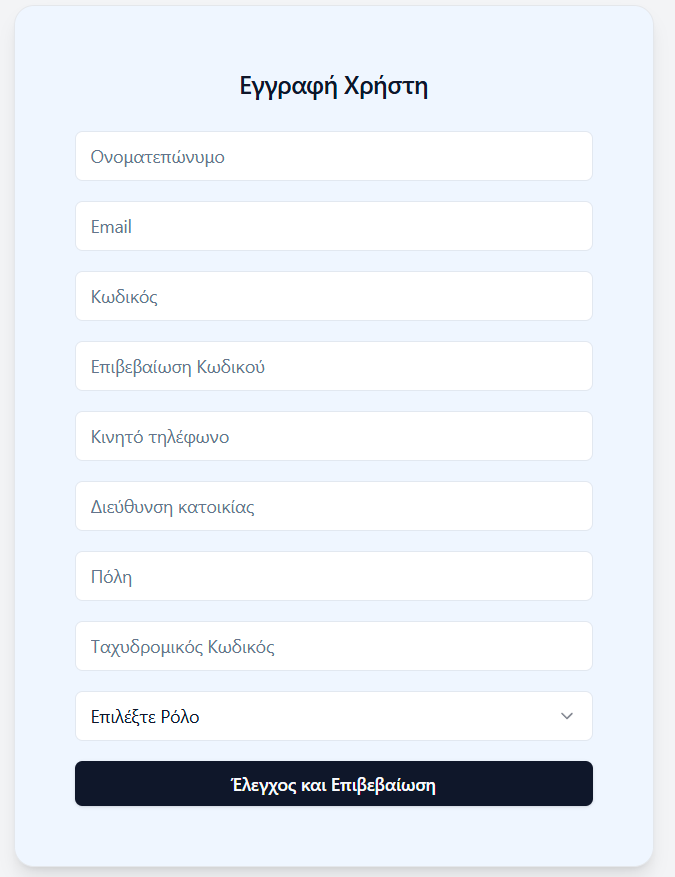
\includegraphics[width=\textwidth]{Mockup Screens/mockup-register.png}
        \caption{Sign Up Screen}\label{fig:mockup1}
    \end{subfigure}
    \hfill
    \begin{subfigure}[b]{0.48\textwidth}
        \centering
        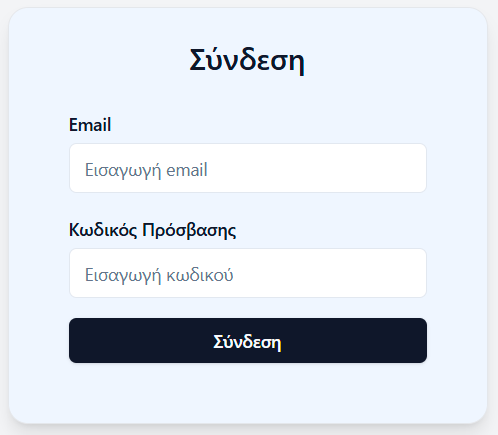
\includegraphics[width=\textwidth]{Mockup Screens/mockup-login1.png}
        \caption{Sign In Screen}\label{fig:mockup2}
    \end{subfigure}
    \caption{Authentication Screens}\label{fig:auth-screens}
\end{figure}

\begin{figure}[H]
    \centering
    \begin{subfigure}[b]{0.48\textwidth}
        \centering
        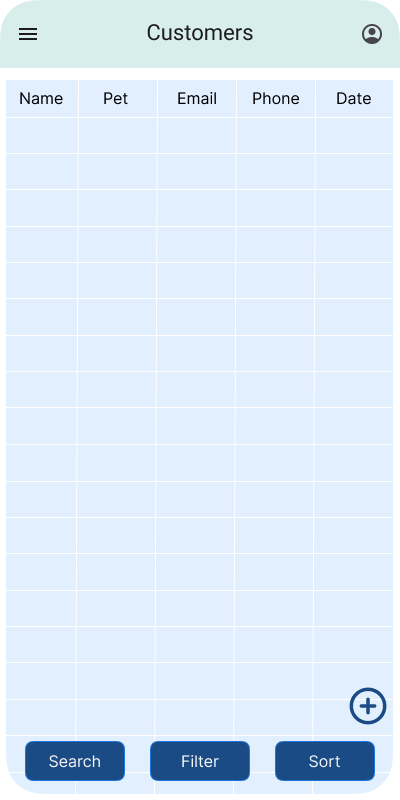
\includegraphics[width=\textwidth,height=0.4\textheight,keepaspectratio]{Mockup Screens/customer_management.png}
        \caption{Customer Management Screen}\label{fig:mockup3}
    \end{subfigure}
    \hfill
    \begin{subfigure}[b]{0.48\textwidth}
        \centering
        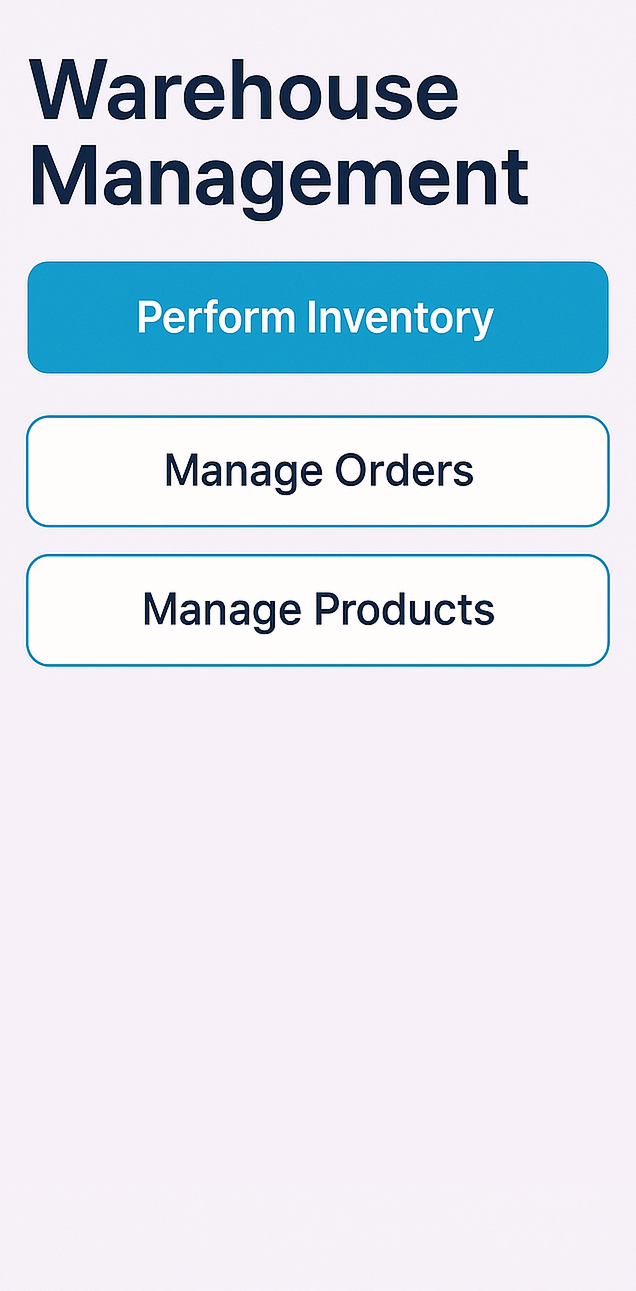
\includegraphics[width=\textwidth,height=0.4\textheight,keepaspectratio]{Mockup Screens/warehouse_management_products.png}
        \caption{Warehouse Management Screen}\label{fig:mockup4}
    \end{subfigure}
\end{figure}

\begin{figure}[H]
    \centering
    \begin{subfigure}[b]{0.48\textwidth}
        \centering
        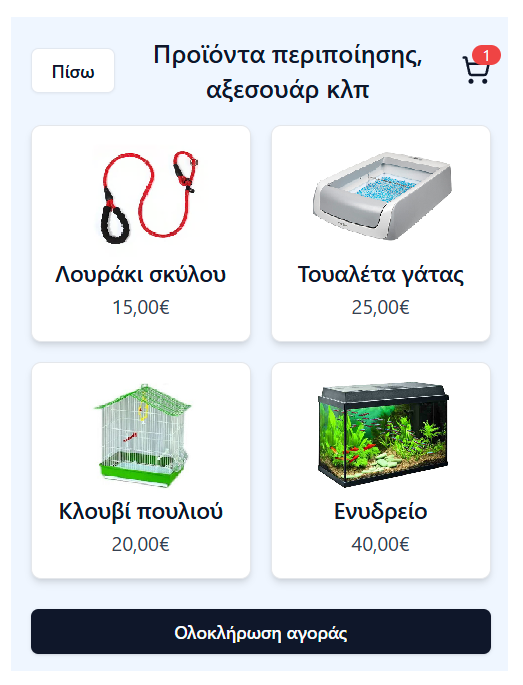
\includegraphics[width=\textwidth]{Mockup Screens/mockup-store.png}
        \caption{Store Screen}\label{fig:mockup5}
    \end{subfigure}
    \hfill
    \begin{subfigure}[b]{0.48\textwidth}
        \centering
        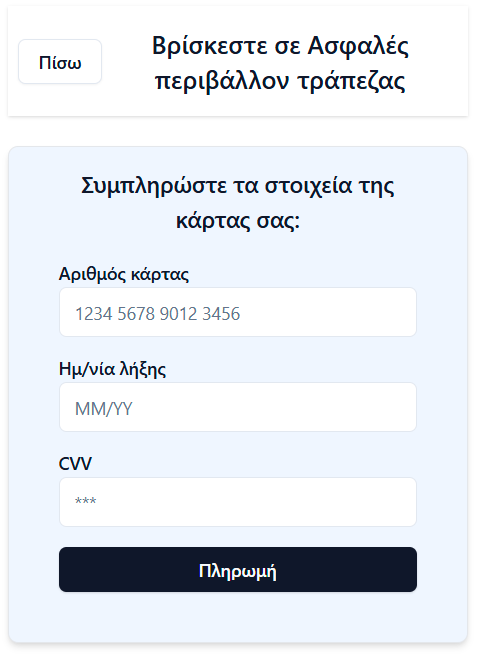
\includegraphics[width=\textwidth]{Mockup Screens/mockup-payment.png}
        \caption{Payment Screen}\label{fig:mockup6}
    \end{subfigure}
\end{figure}

\begin{figure}[H]
    \centering
    \begin{subfigure}[b]{0.48\textwidth}
        \centering
        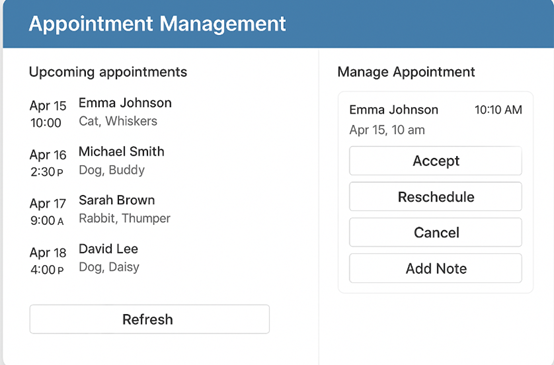
\includegraphics[width=\textwidth]{Mockup Screens/Appointment_Management.png}
        \caption{Appointment Management Screen}\label{fig:mockup7}
    \end{subfigure}
    \hfill
    \begin{subfigure}[b]{0.48\textwidth}
        \centering
        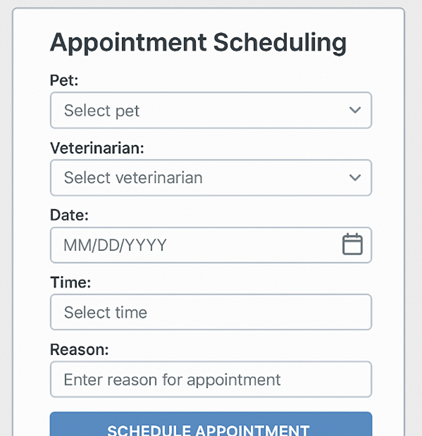
\includegraphics[width=\textwidth]{Mockup Screens/Appointment_Scheduling.png}
        \caption{Appointment Scheduling Screen}\label{fig:mockup8}
    \end{subfigure}
\end{figure}

\begin{figure}[H]
    \centering
    \begin{subfigure}[b]{0.48\textwidth}
        \centering
        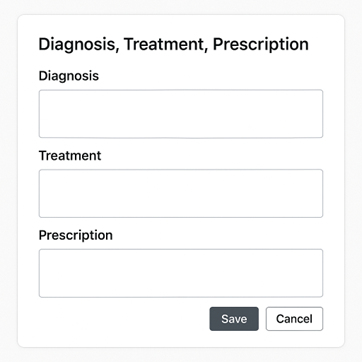
\includegraphics[width=\textwidth]{Mockup Screens/Diagnosis.png}
        \caption{Medical Record Screen}\label{fig:mockup9}
    \end{subfigure}
    \hfill
    \begin{subfigure}[b]{0.48\textwidth}
        \centering
        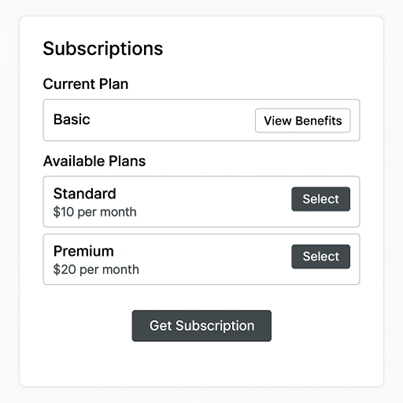
\includegraphics[width=\textwidth]{Mockup Screens/Subscription.png}
        \caption{Subscriptions Screen}\label{fig:mockup10}
    \end{subfigure}
\end{figure}

\begin{figure}[H]
    \centering
    \begin{subfigure}[b]{0.48\textwidth}
        \centering
        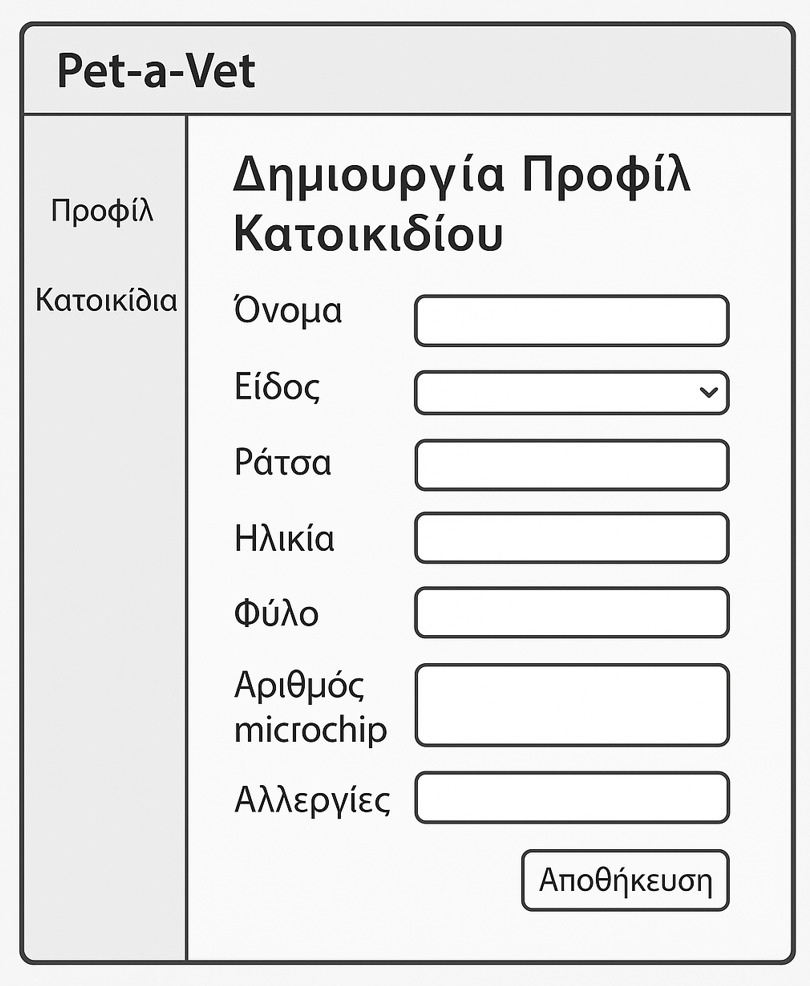
\includegraphics[width=\textwidth]{Mockup Screens/Pet_profile.png}
        \caption{Profile Creation for Pets Screen}\label{fig:mockup11}
    \end{subfigure}
    \hfill
    \begin{subfigure}[b]{0.48\textwidth}
        \centering
        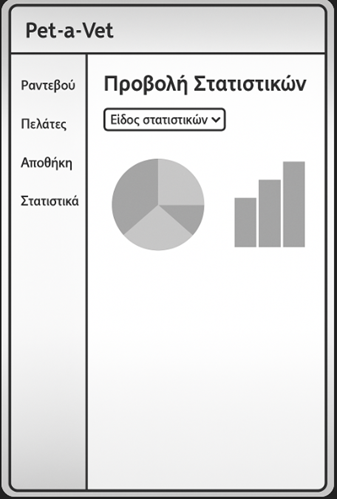
\includegraphics[width=\textwidth]{Mockup Screens/View_statistics.png}
        \caption{View Statistics Screen}\label{fig:mockup12}
    \end{subfigure}
\end{figure}

\subsection{Παραδοχές} % chktex 19

Χρησιμοποιήθηκε Generative Artificial Intelligence \textit{(Text-to-Image)}, σε συνδυασμό με το εργαλείο \textit{Figma} σε κάποιες περιπτώσεις, για την παραγωγή των παραπάνω οθονών, ενώ σε κάποιες άλλες αναπτύχθηκε σύντομος κώδικας. % chktex 19

\chapter{Sequence-diagram-v0.1}

\section{Διαγράμματα Ακολουθίας}

Παρακάτω παρατίθενται τα διαγράμματα ακολουθίας για την εφαρμογή \textit{Pet-à-Vet} με τη σειρά που εμφανίζονται και οι περιπτώσεις χρήσης. Χρησιμοποιήθηκε το εργαλείο Visual Paradigm για την σχεδίαση των διαγραμμάτων, με την βοήθεια και επίβλεψη όλων των μελών της ομάδας. Προκειμένου τα διαγράμματα να είναι ευανάγνωστα, οι χειριστές θα παρατίθονται στα υπομνήματα των διαγραμμάτων. % chktex 19

\subsection{Sign Up}
\begin{figure}[H]
    \centering
    \includegraphics[width=0.8\textwidth]{}
    \caption{User είναι Διαχειριστής, Γραμματέας, Κτηνίατρος, Pet Groomer και Πελάτης}\label{fig:sequence-signup}
\end{figure}

\subsection{Sign In}
\begin{figure}[H]
    \centering
    \includegraphics[width=0.8\textwidth]{}
    \caption{User είναι Διαχειριστής, Γραμματέας, Κτηνίατρος, Pet Groomer και Πελάτης}\label{fig:sequence-signin}
\end{figure}

\subsection{Customer Management}
\begin{figure}[H]
    \centering
    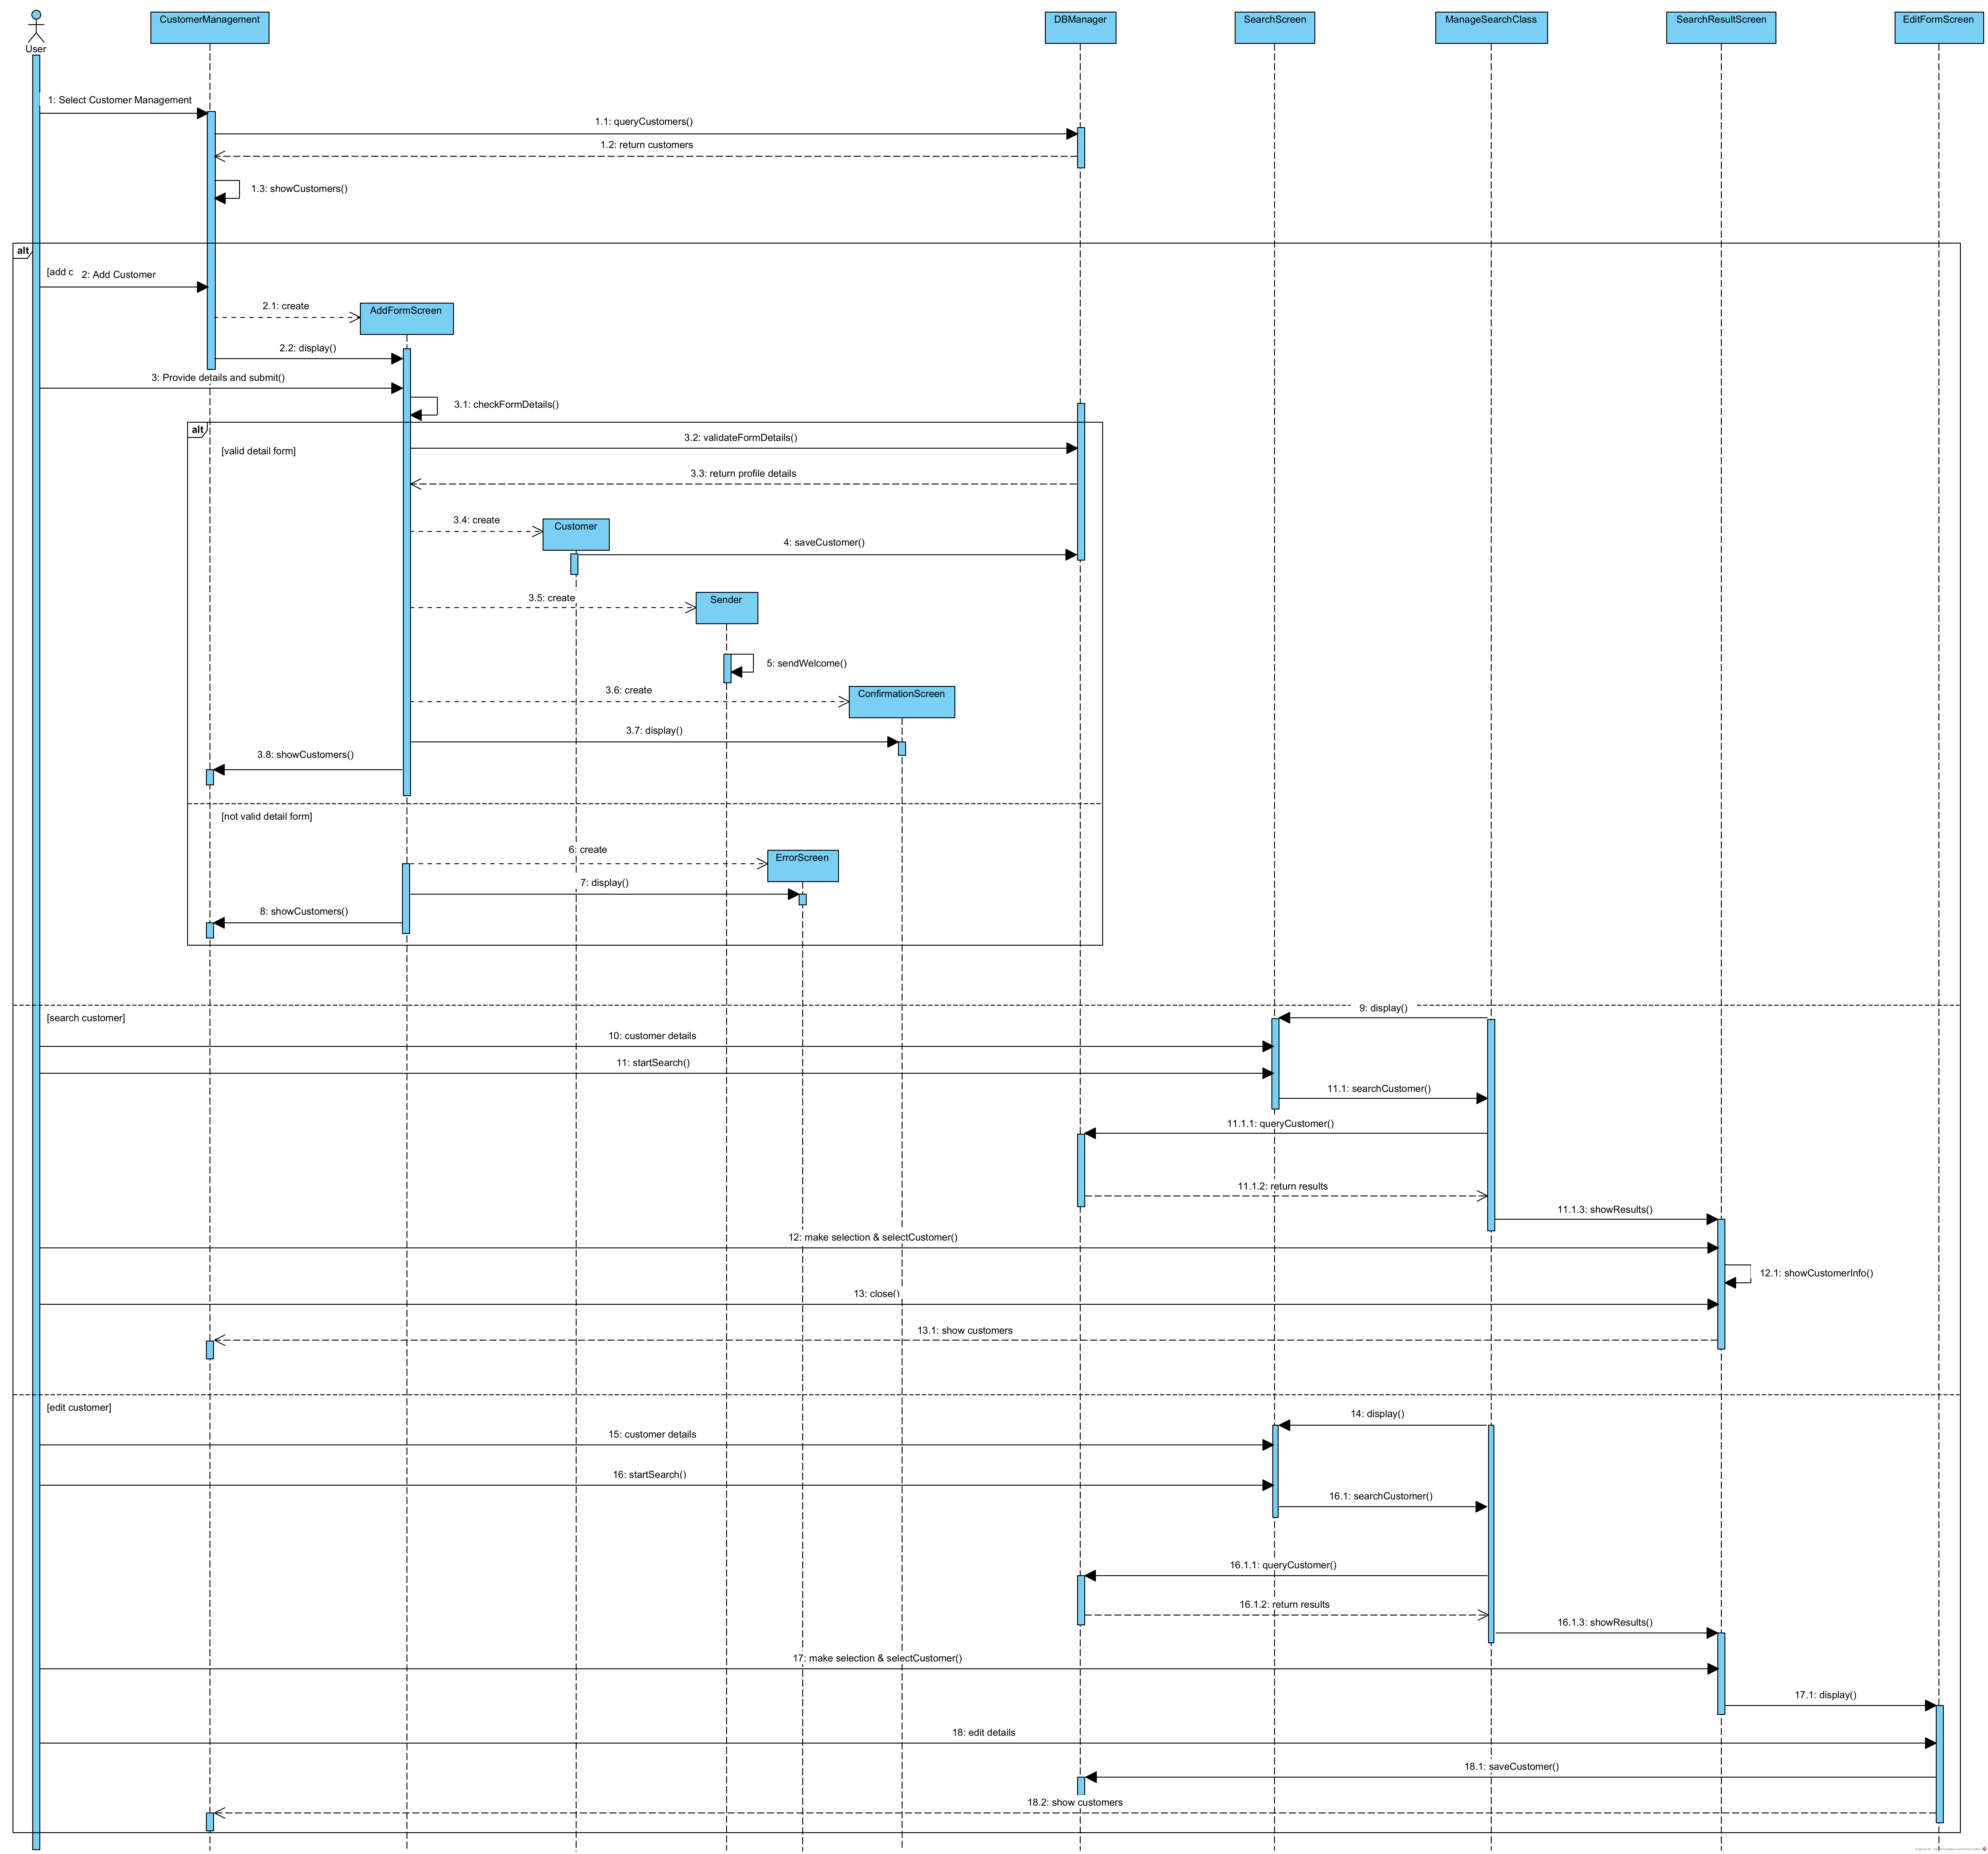
\includegraphics[width=\textwidth]{Resources/Sequence Diagram/customer_management_sd.png}
    \caption{User είναι Διαχειριστής και Γραμματέας}\label{fig:sequence-customer-management}
\end{figure}

\subsection{Filter}
\begin{figure}[H]
    \centering
    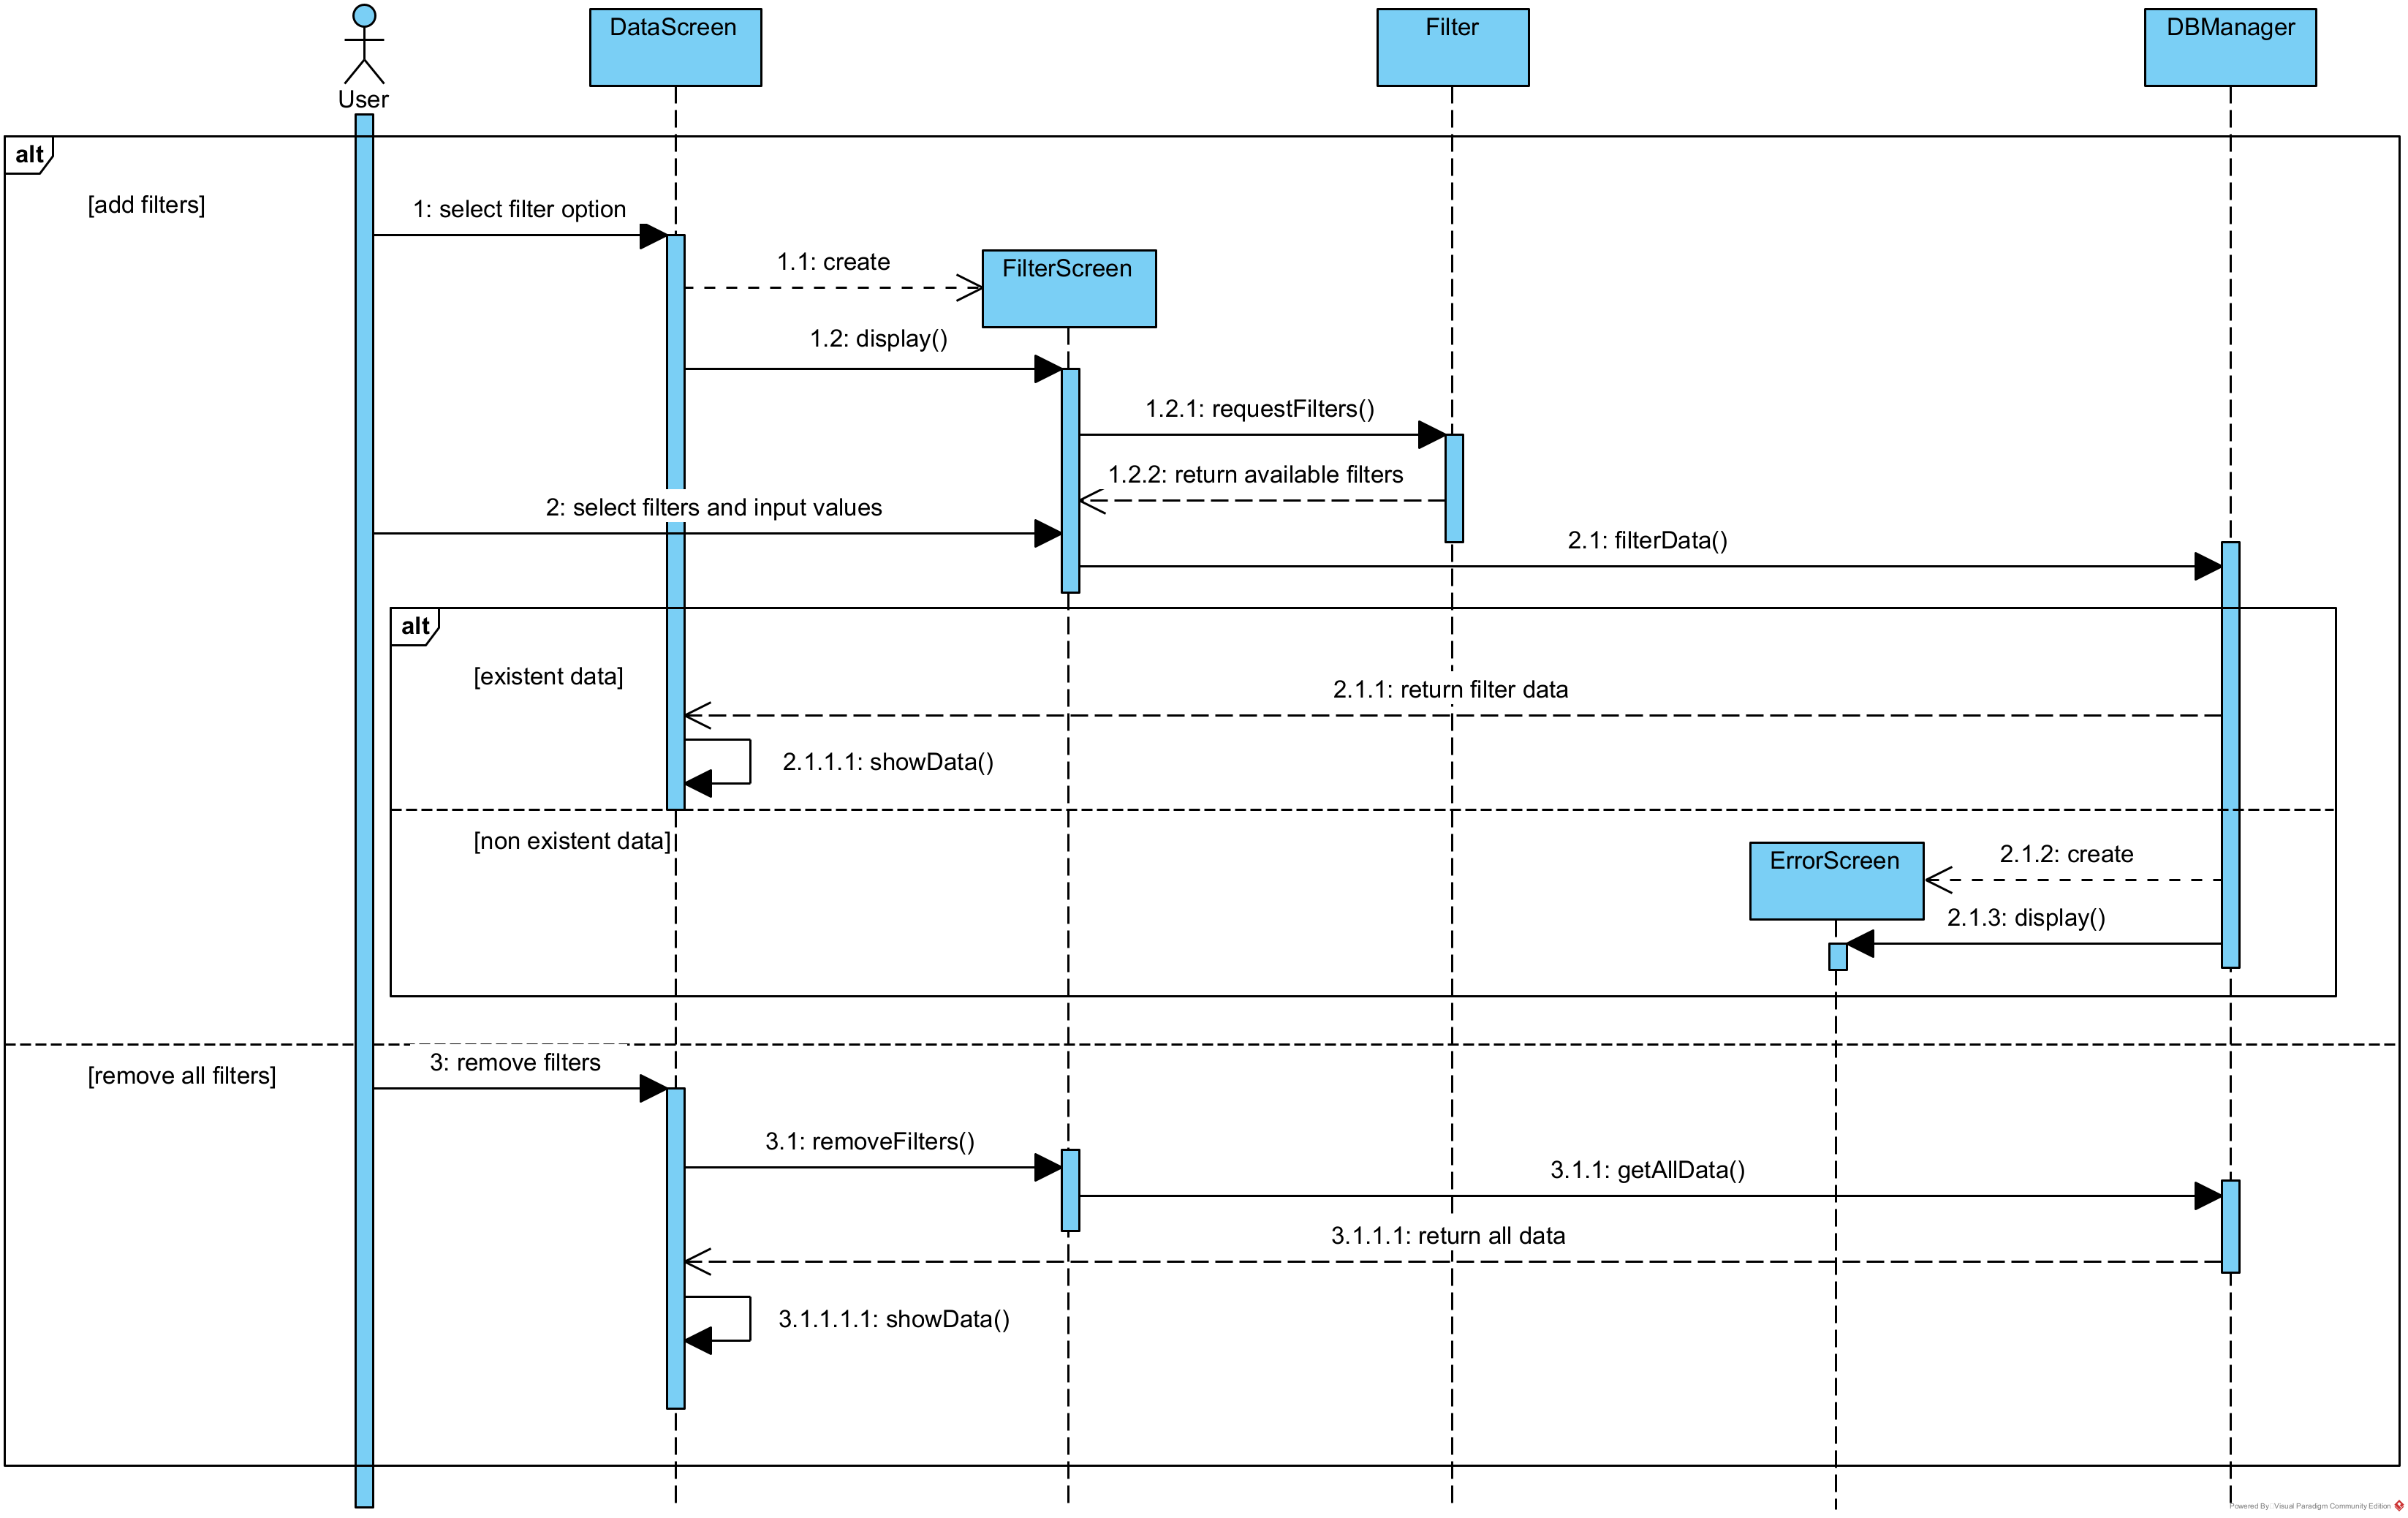
\includegraphics[width=\textwidth]{Resources/Sequence Diagram/filter_sd.png}
    \caption{User είναι Διαχειριστής, Γραμματέας, Κτηνίατρος και Πελάτης}\label{fig:sequence-filter}
\end{figure}

\subsection{Warehouse Management}
\begin{figure}[H]
    \centering
    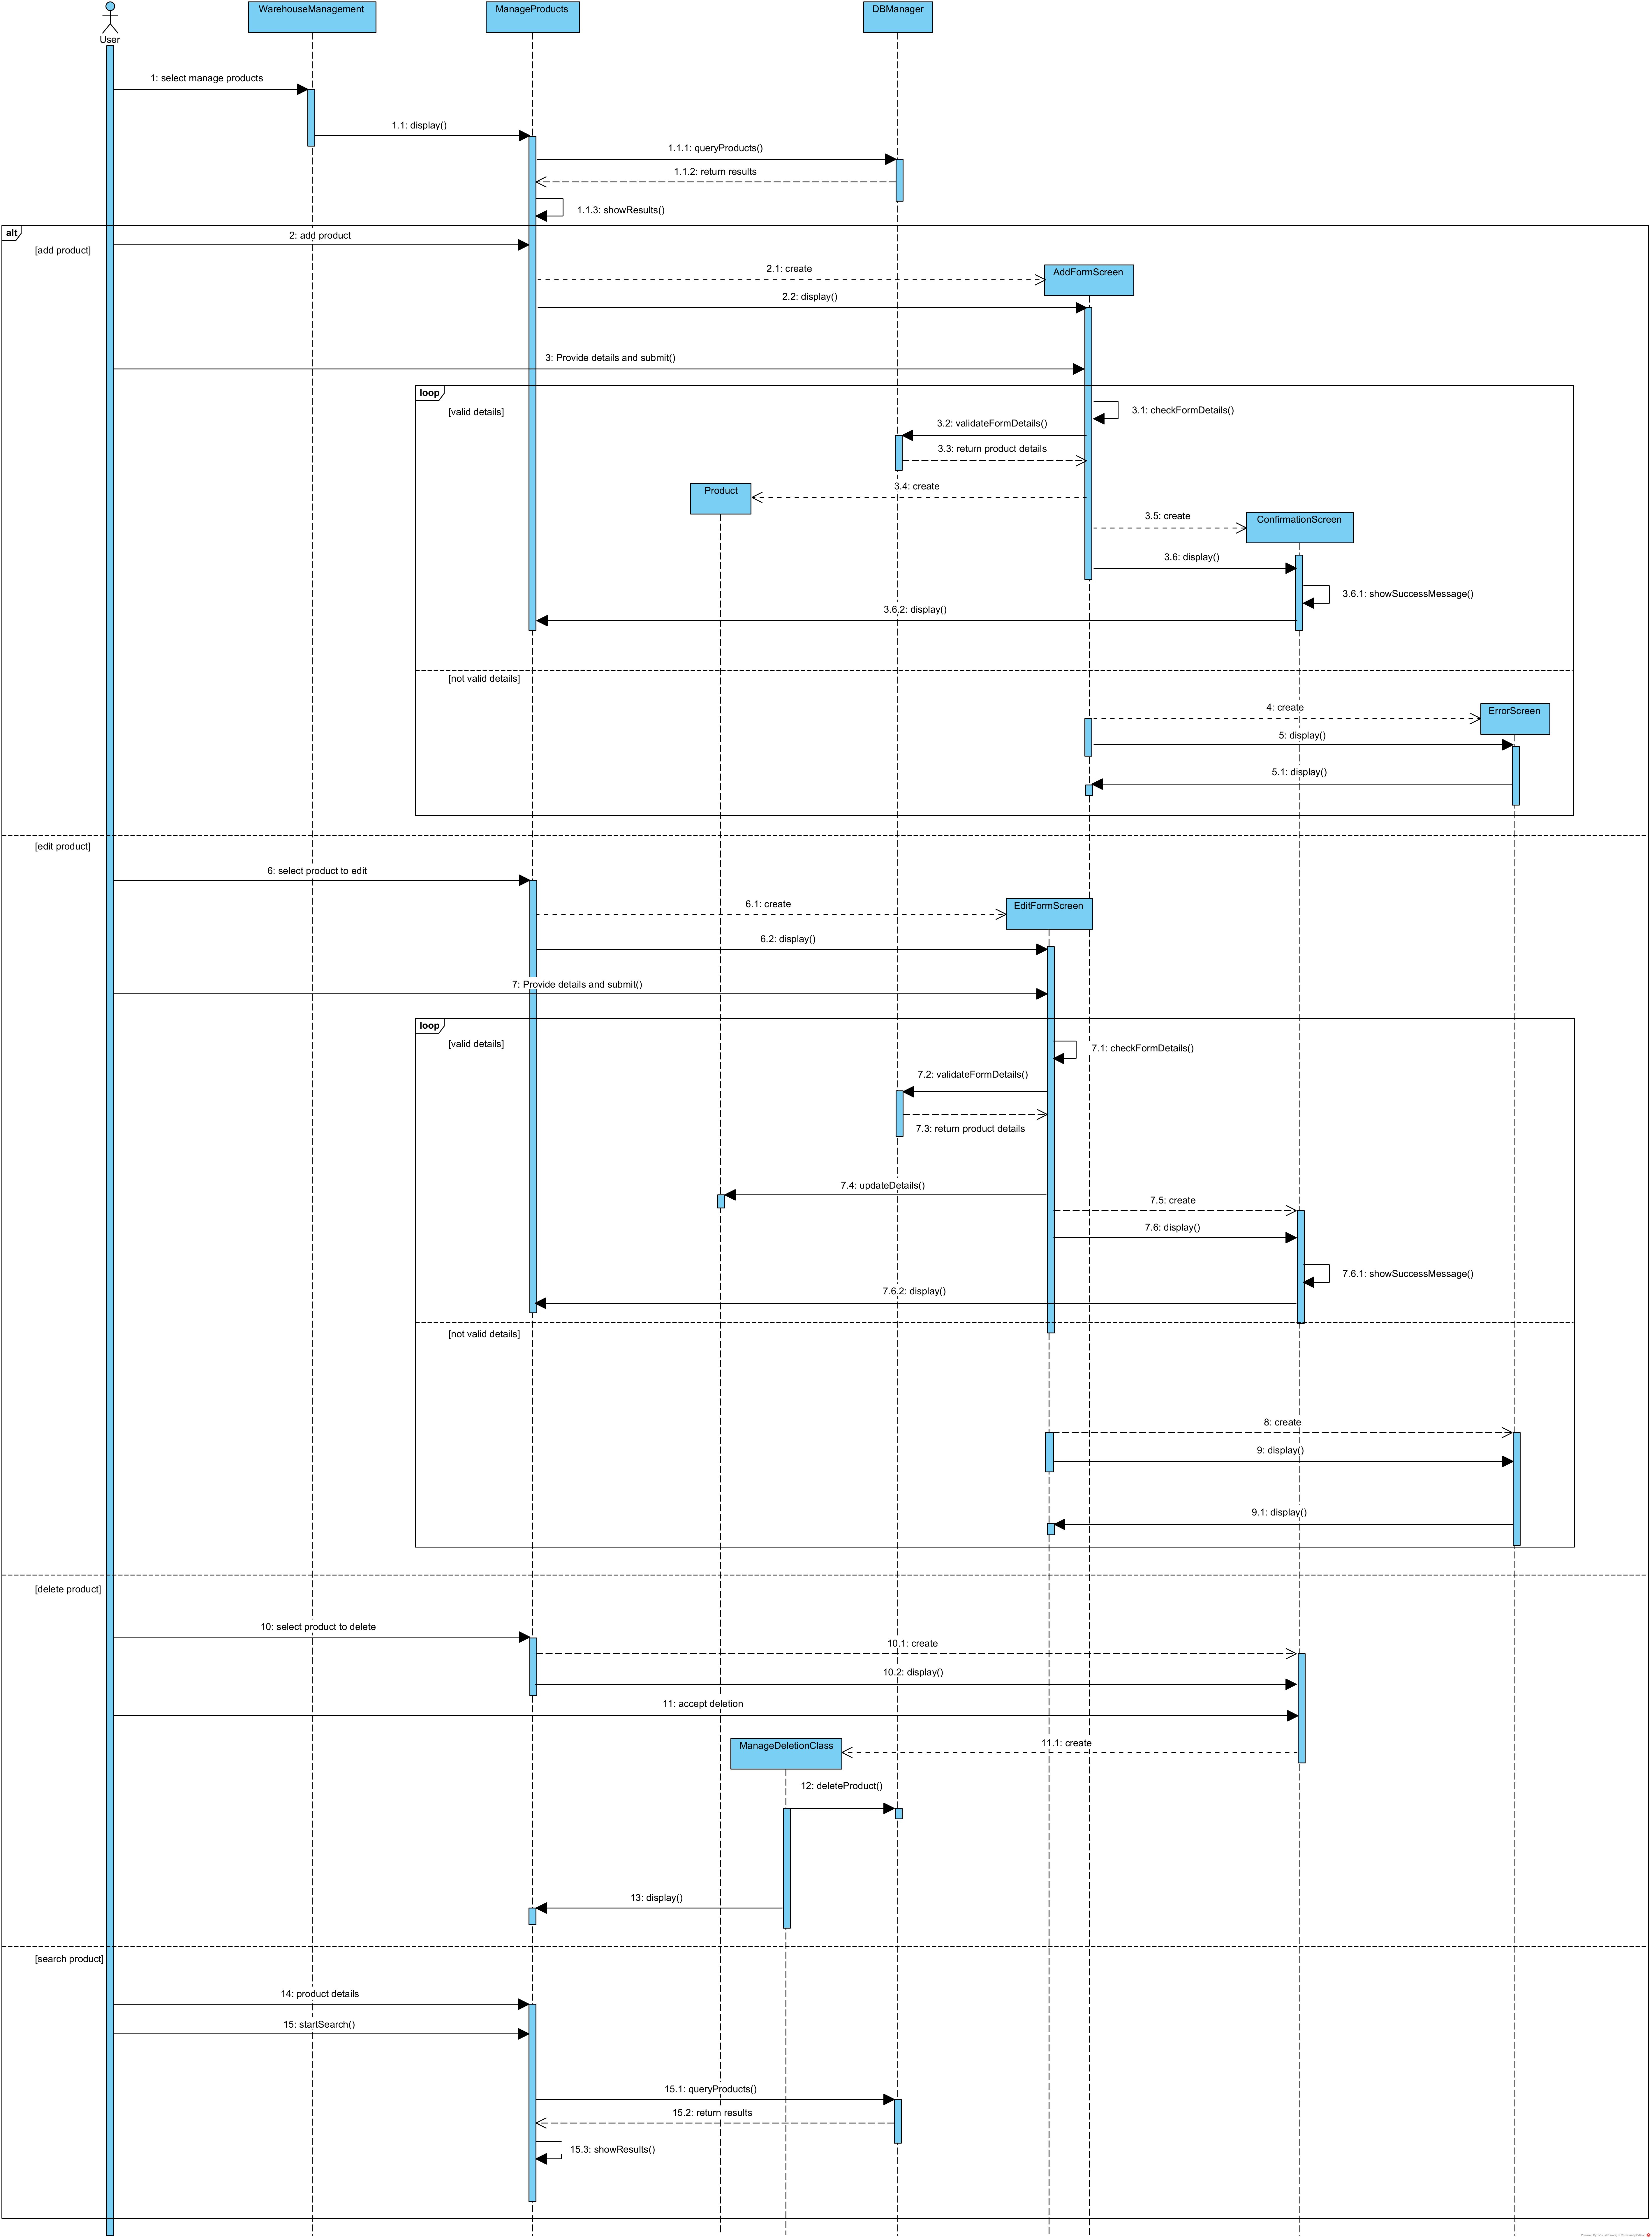
\includegraphics[width=\textwidth]{Resources/Sequence Diagram/warehouse_management_sd.png}
    \caption{User είναι Διαχειριστής, Κτηνίατρος και Γραμματέας}\label{fig:sequence-warehouse-management}
\end{figure}

\subsection{Perform Inventory}
\begin{figure}[H]
    \centering
    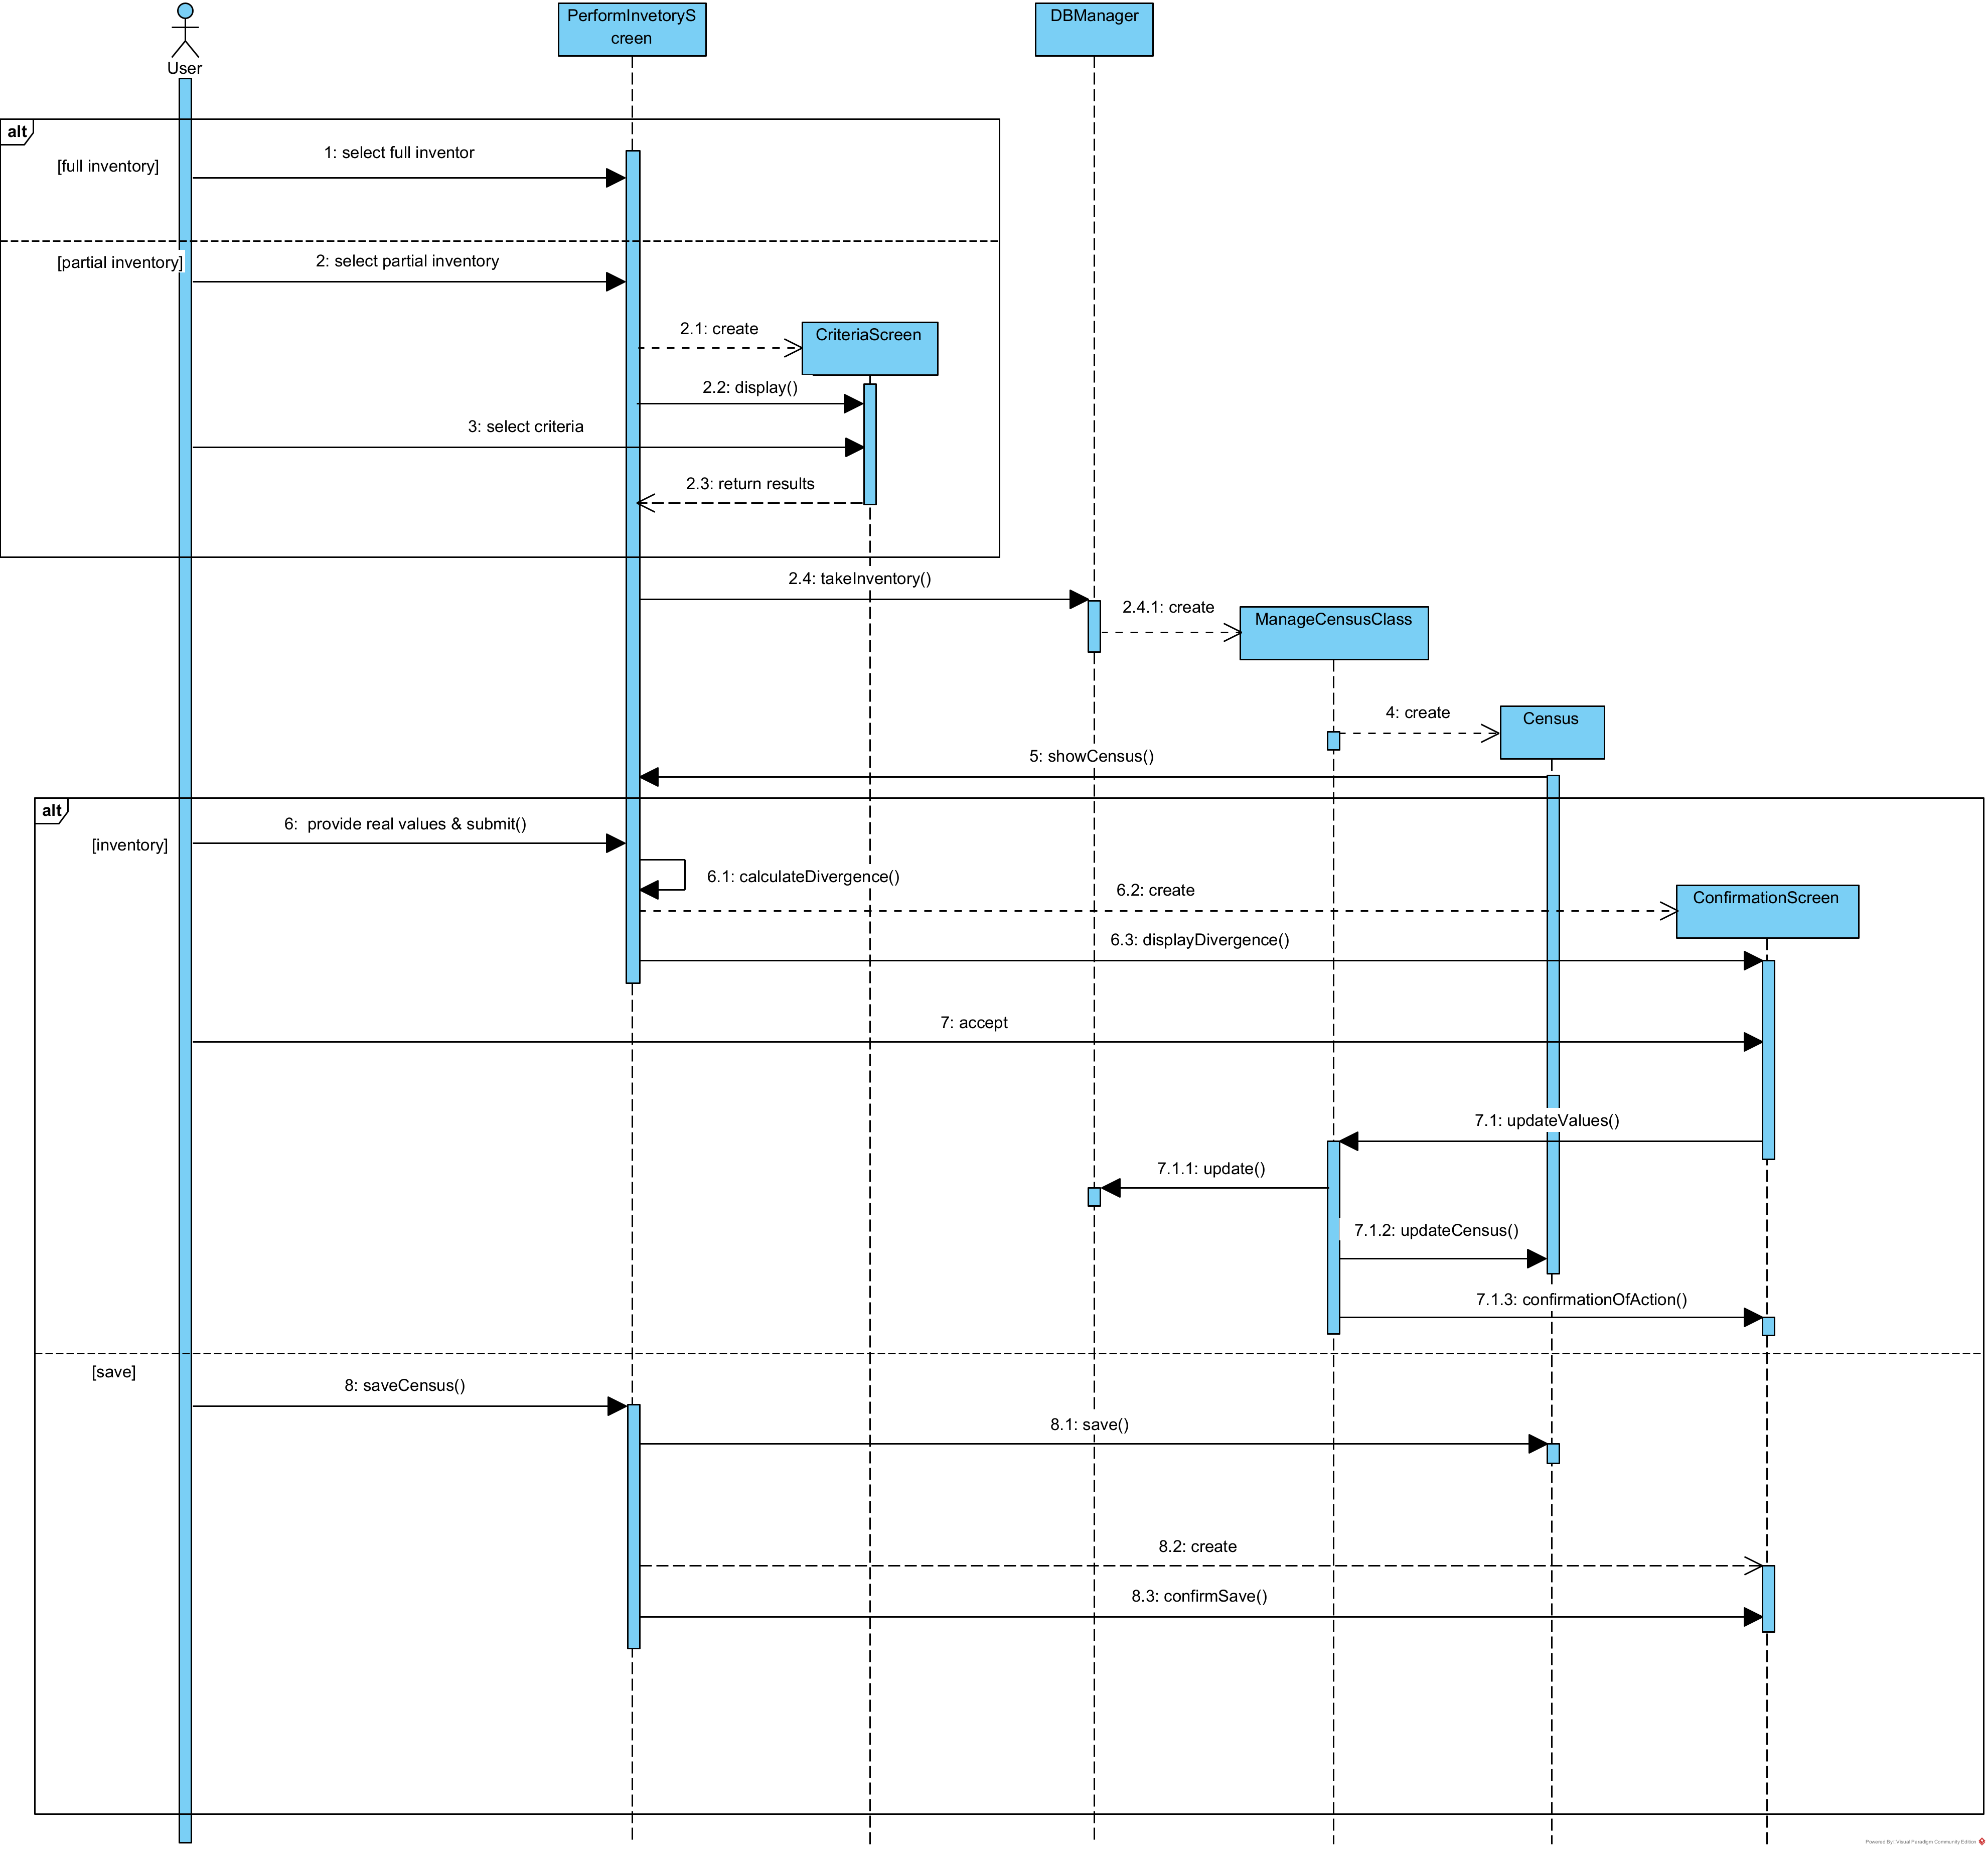
\includegraphics[width=\textwidth]{Resources/Sequence Diagram/perform_inventory_sd.png}
    \caption{User είναι Διαχειριστής, Κτηνίατρος και Γραμματέας}\label{fig:sequence-perform-inventory}
\end{figure}

\subsection{Manage Orders}
\begin{figure}[H]
    \centering
    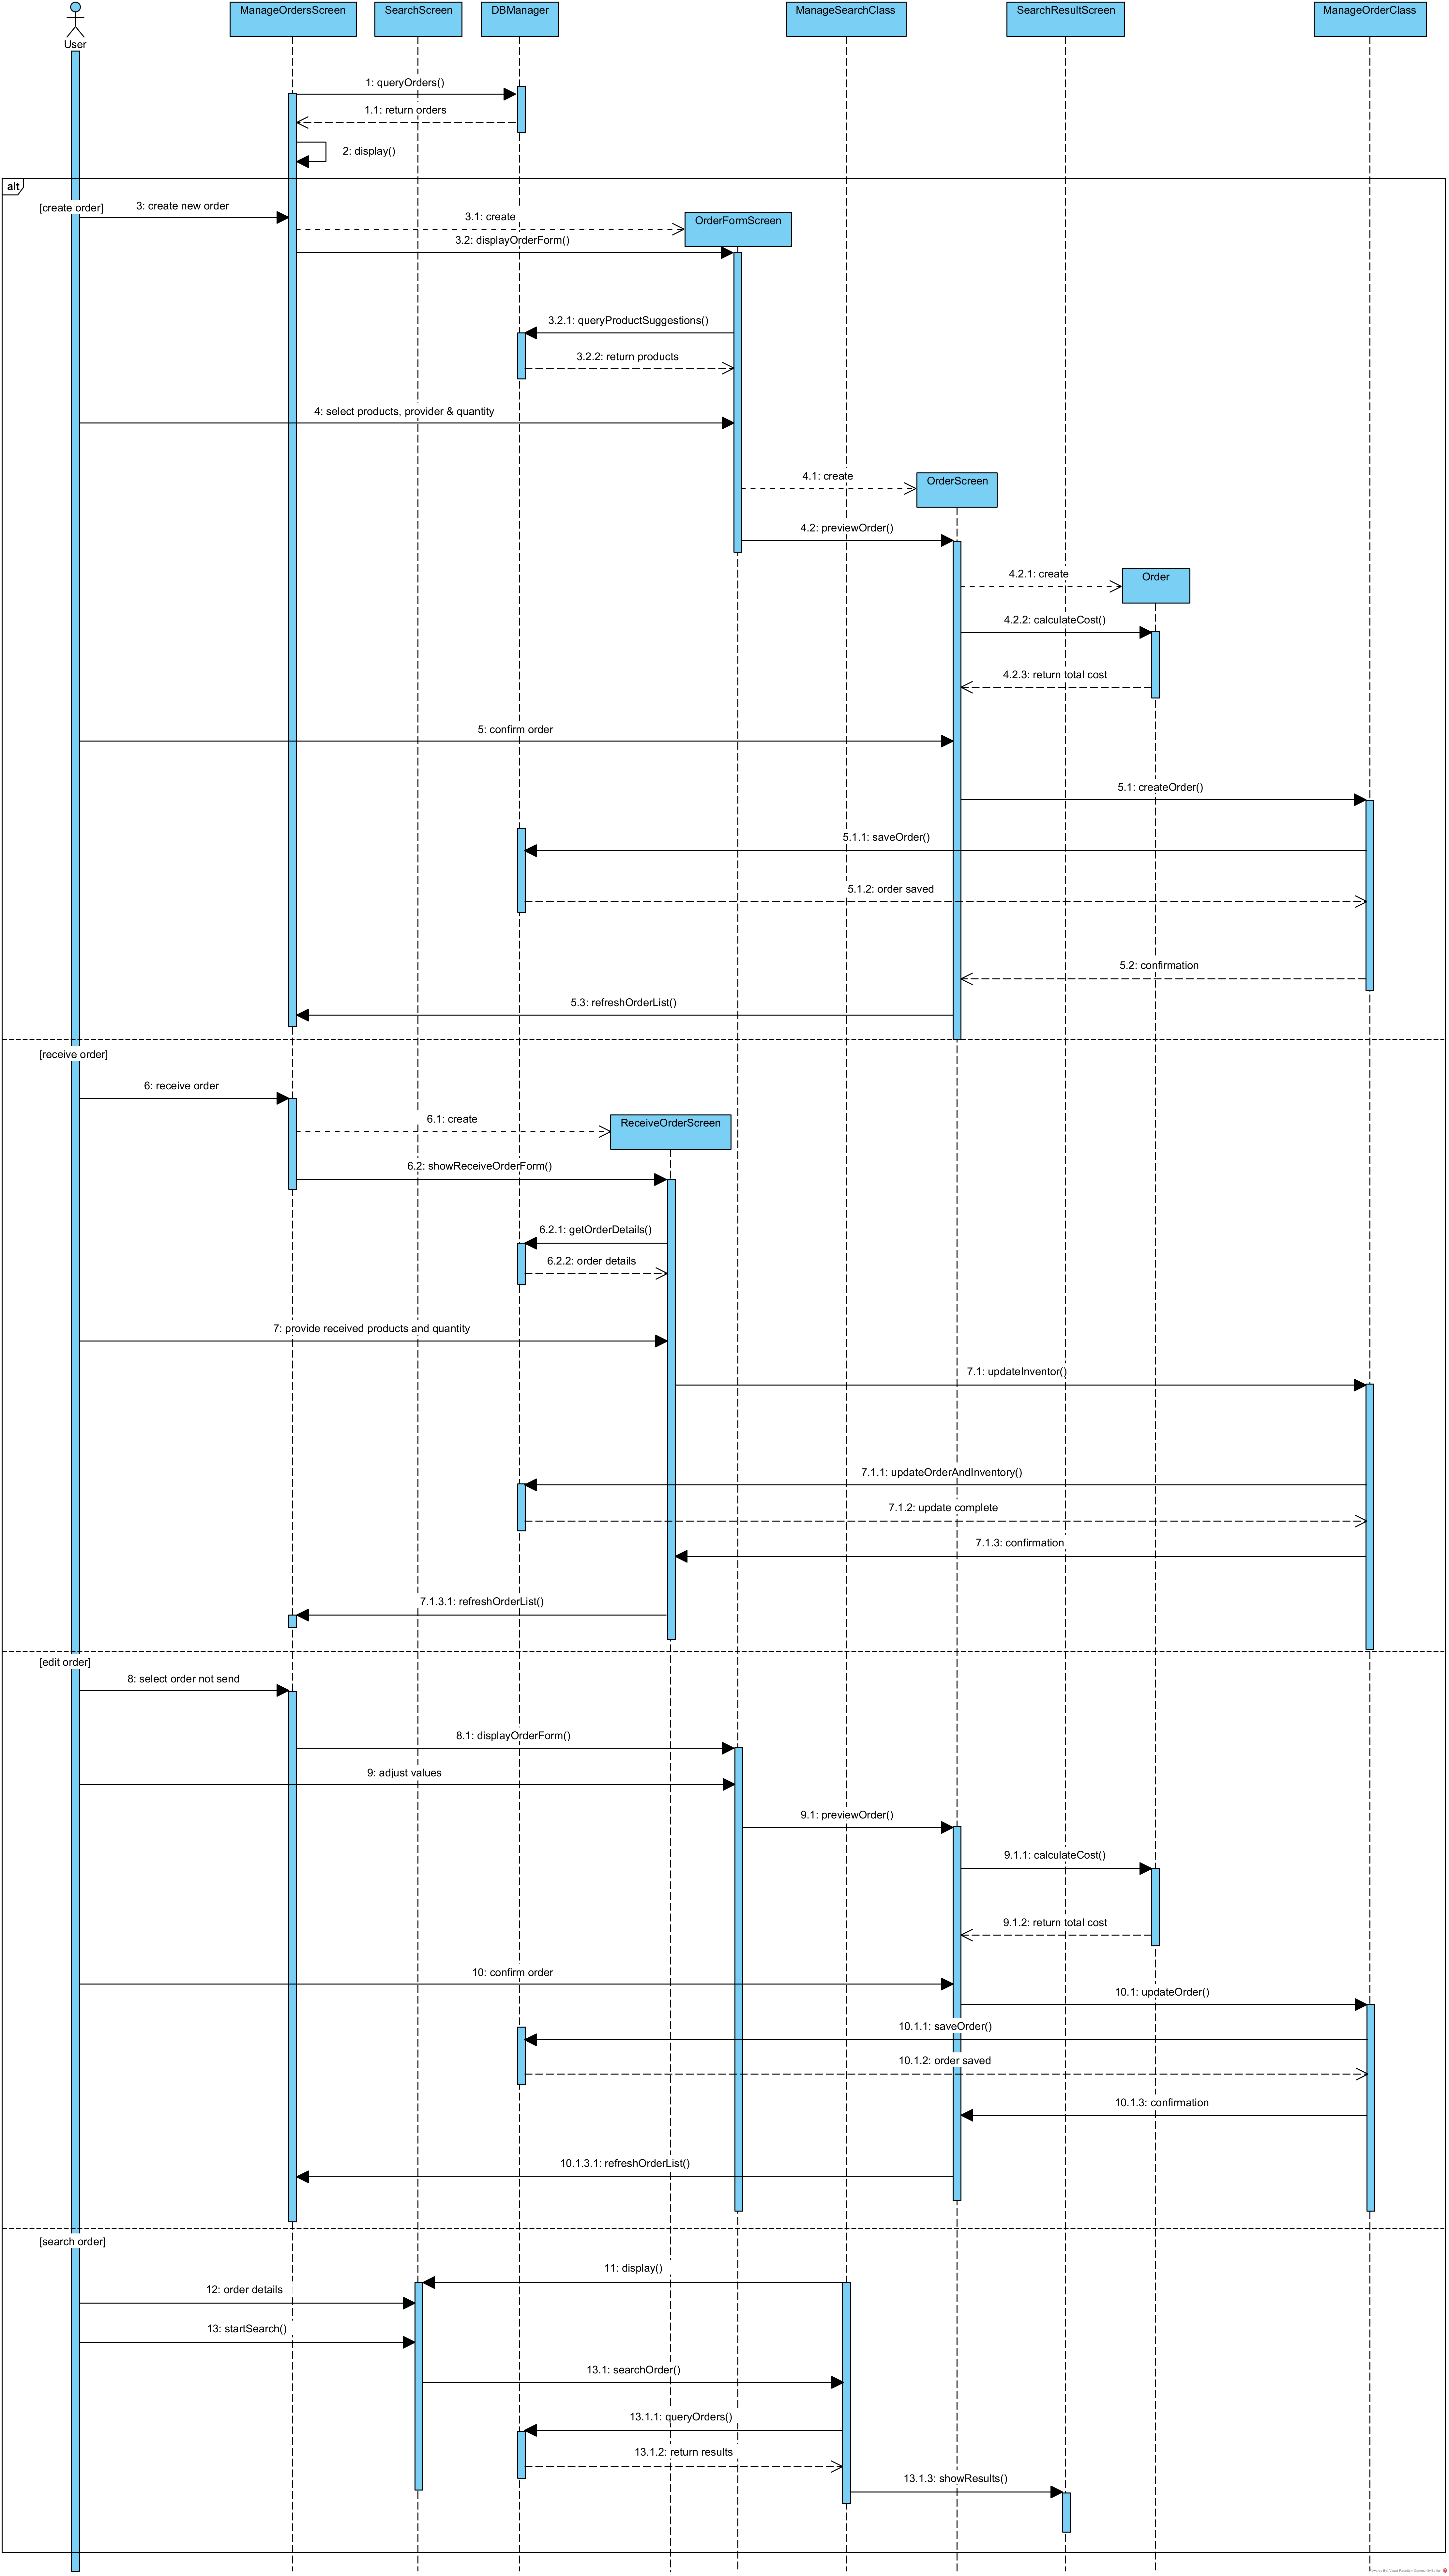
\includegraphics[width=0.8\textwidth]{Resources/Sequence Diagram/manage_orders_sd.png}
    \caption{User είναι Διαχειριστής, Κτηνίατρος και Γραμματέας}\label{fig:sequence-manage-orders}
\end{figure}

\subsection{Store}
\begin{figure}[H]
    \centering
    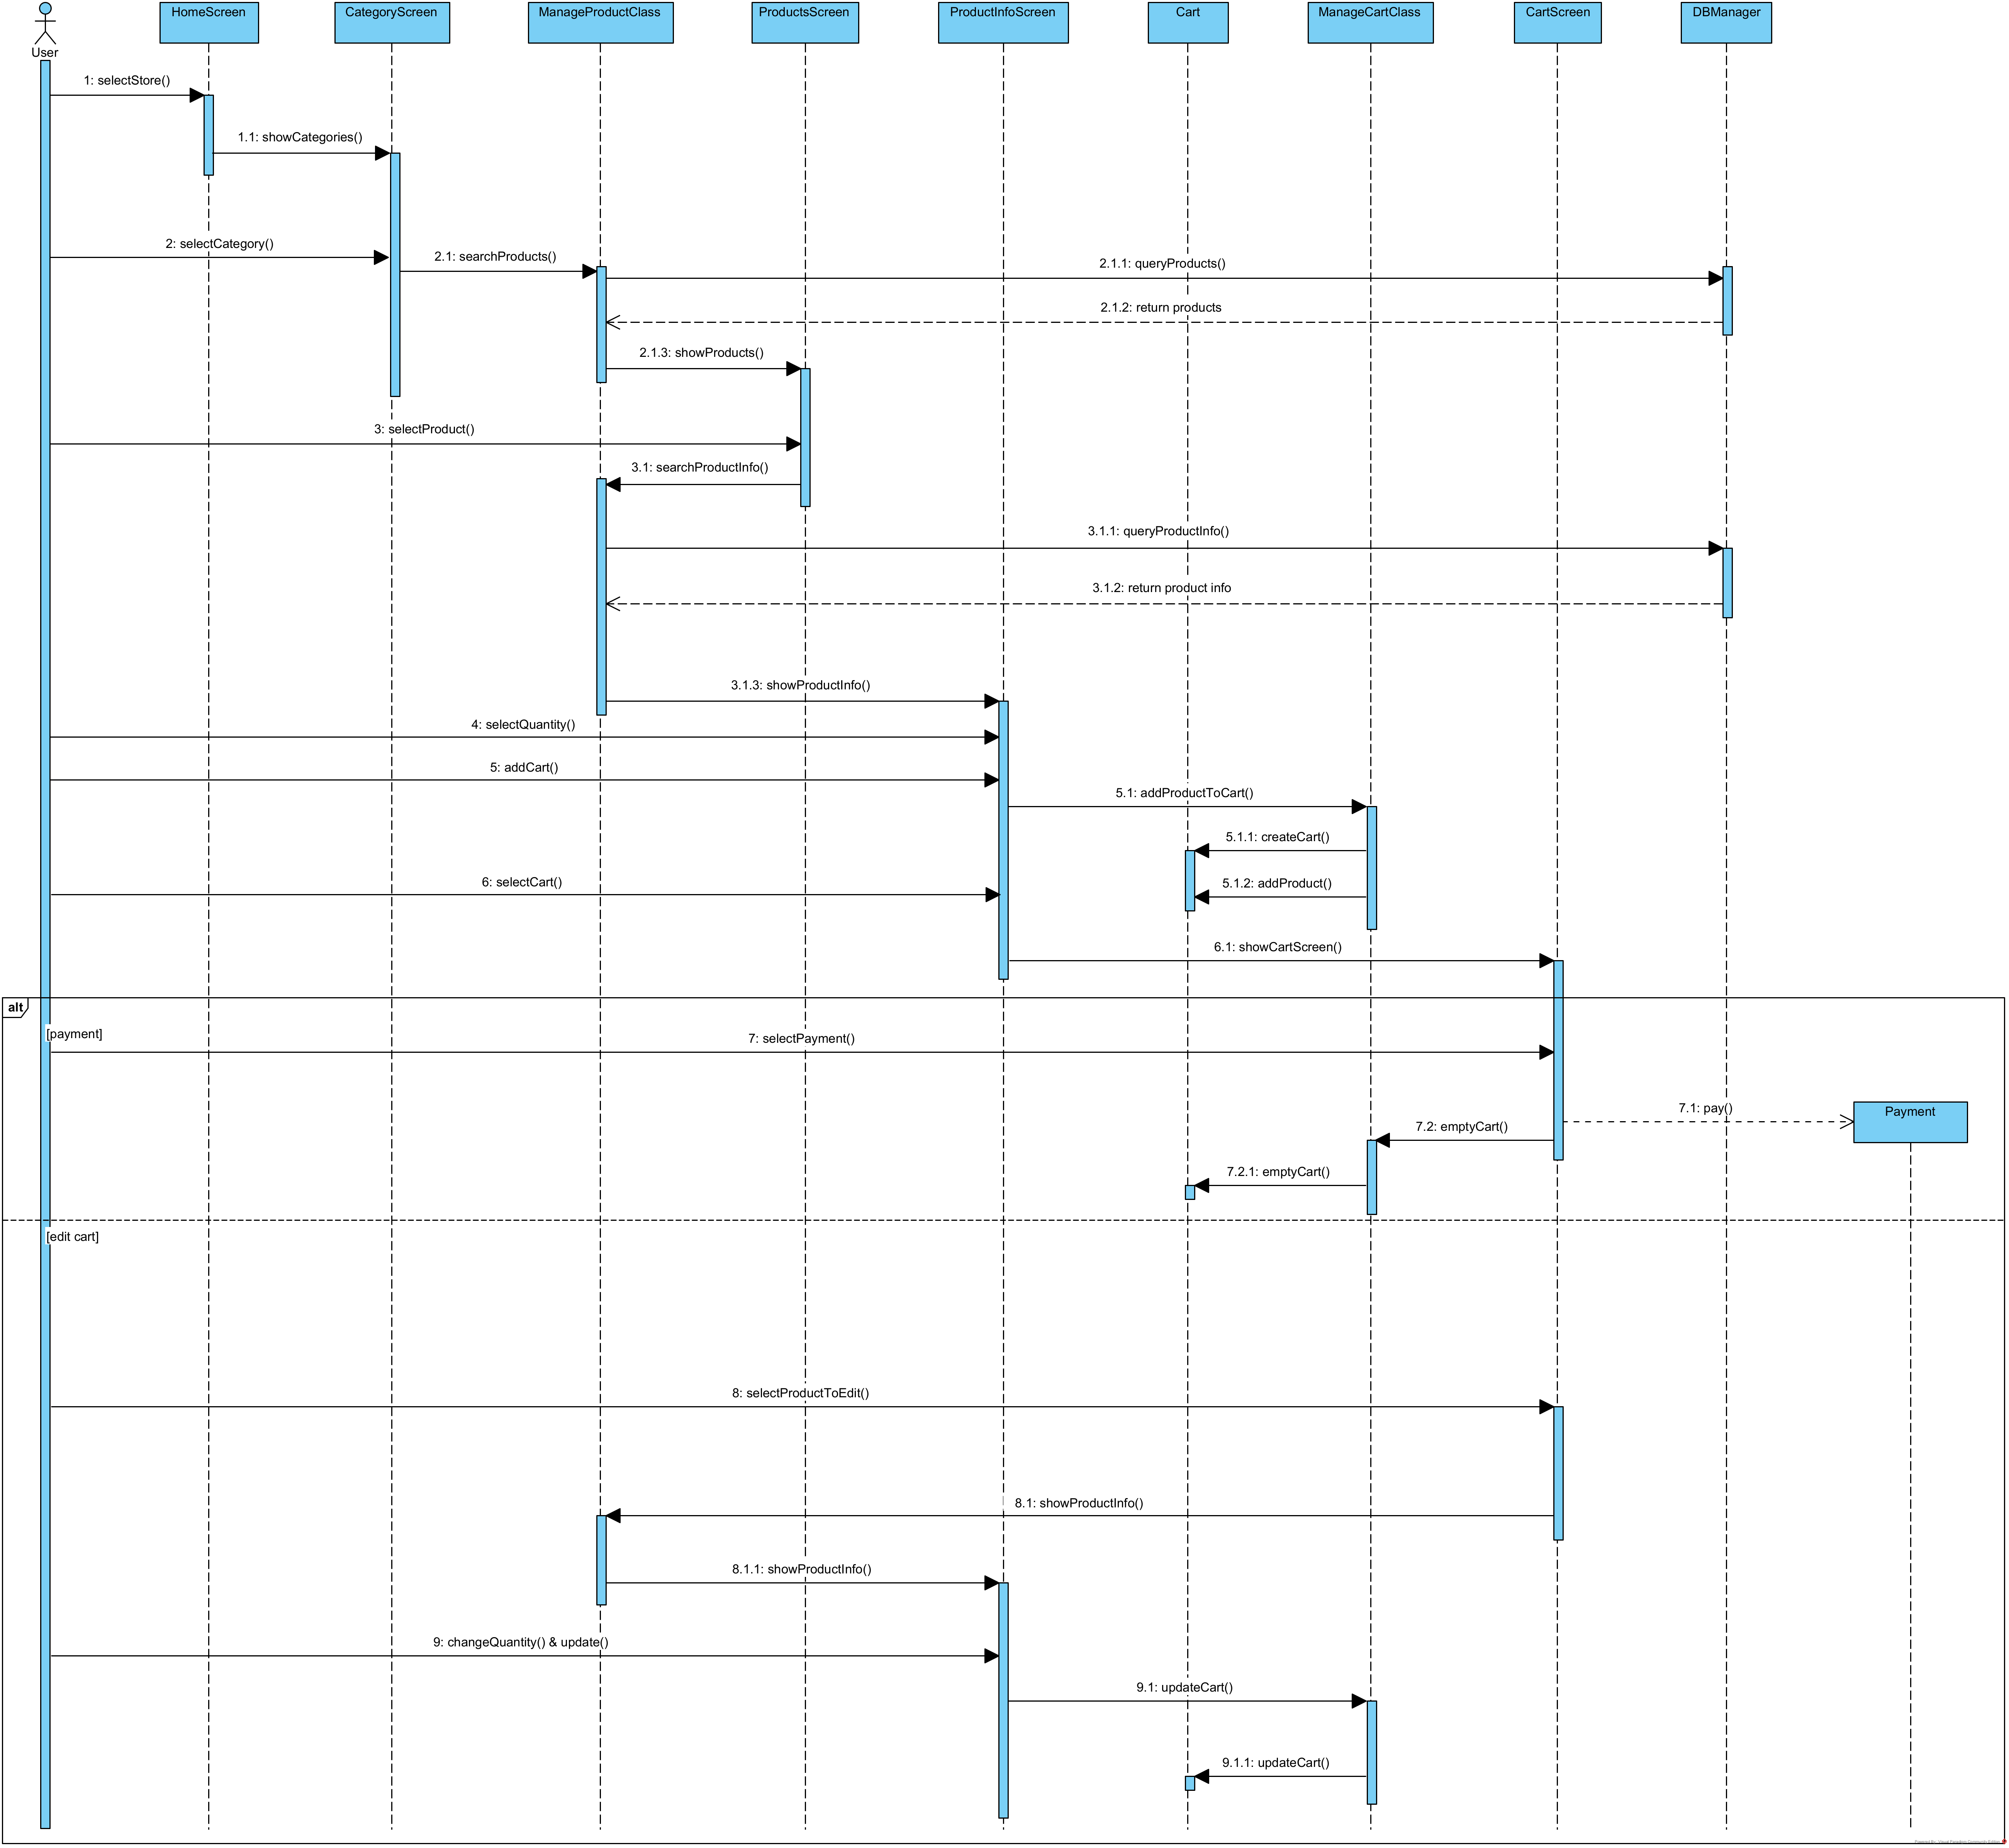
\includegraphics[width=0.8\textwidth]{Resources/Sequence Diagram/Store_sd.png.png}
    \caption{User είναι Διαχειριστής και Πελάτης}\label{fig:sequence-store}
\end{figure}

\subsection{Payment}
\begin{figure}[H]
    \centering
    \includegraphics[width=0.8\textwidth]{}
    \caption{User είναι Διαχειριστής και Πελάτης}\label{fig:sequence-payment}
\end{figure}

\subsection{Appointment Management}
\begin{figure}[H]
    \centering
    \includegraphics[width=\textwidth]{}
    \caption{Actor είναι Διαχειριστής, Γραμματέας, Pet Groomer και Κτηνίατρος}\label{fig:sequence-appointment-management}
\end{figure}

\subsection{Appointment Scheduling}
\begin{figure}[H]
    \centering
    \includegraphics[width=\textwidth]{}\label{fig:sequence-appointment-scheduling}
\end{figure}

\subsection{MedicalRecord}
\begin{figure}[H]
    \centering
    \includegraphics[width=\textwidth]{}
    \caption{User είναι Διαχειριστής, Πελάτης και Κτηνίατρος}\label{fig:sequence-medical-record}
\end{figure}

\subsection{Subscriptions}
\begin{figure}[H]
    \centering
    \includegraphics[width=\textwidth]{}
    \caption{User είναι Διαχειριστής και Πελάτης}\label{fig:sequence-subscription}
\end{figure}

\subsection{Pet's Profile Creation}
\begin{figure}[H]
    \centering
    \includegraphics[width=\textwidth]{}
    \caption{User είναι Διαχειριστής, Κτηνίατρος και Πελάτης}\label{fig:sequence-pet-profile}
\end{figure}

\subsection{View Statistics}
\begin{figure}[H]
    \centering
    \includegraphics[width=\textwidth]{}
    \caption{User είναι Διαχειριστής, Κτηνίατρος, Pet Groomer και Γραμματέας}\label{fig:sequence-view-statistics}
\end{figure}

\chapter{Robustness-diagram-v0.2}

\section{Διαγράμματα Ευρωστίας}

Παρακάτω παρατίθονται τα διαγράμματα ευρωστίας για την εφαρμογή \textit{Pet-à-Vet} με τη ίδια σειρά που εμφανίζονται και οι περιπτώσεις χρήσης. Χρησιμοποιήθηκε το εργαλείο Visual Paradigm για την σχεδίαση των διαγραμμάτων, με την βοήθεια και επίβλεψη όλων των μελών της ομάδας. Προκειμένου τα διαγράμματα να είναι ευανάγνωστα, οι χειριστές θα παρατίθονται στα υπομνήματα των διαγραμμάτων. % chktex 19

Στη δεύτερη έκδοση, τα διαγράμματα ευρωστίας έχουν αναθεωρηθεί και βελτιωθεί, αφαιρώντας ή προσθέτοντας ελεγκτές και ενέργεις των χειριστών, για καλύτερη αναπαράσταση των περιπτώσεων χρήσης. % chktex 19

\subsection{Sign Up}
\begin{figure}[H]
    \centering
    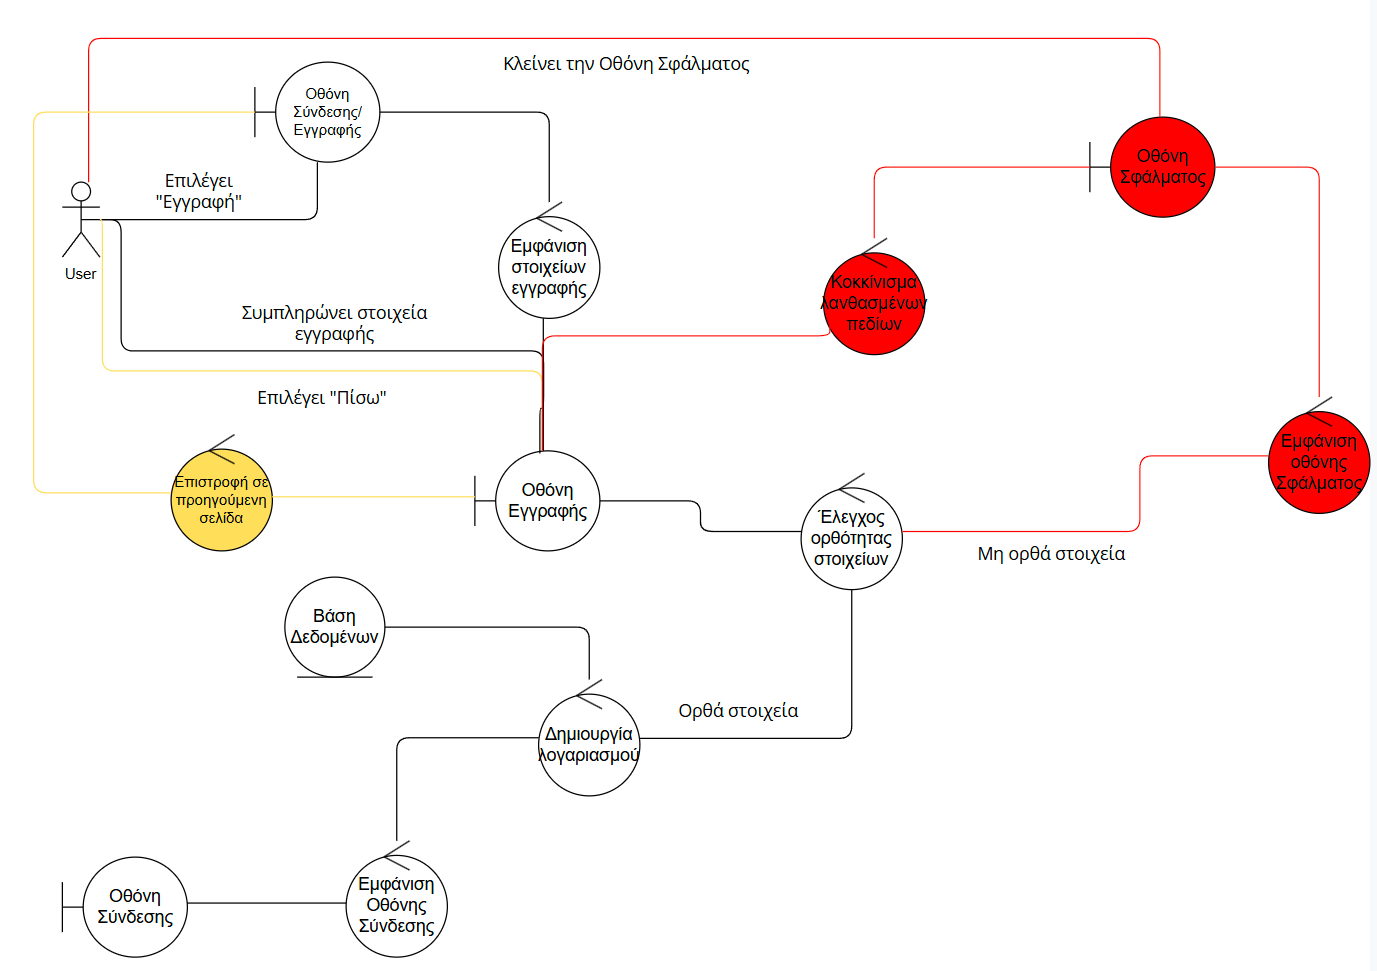
\includegraphics[width=0.8\textwidth]{Resources/Robustness Diagram/SignUp.png}
    \caption{User είναι Διαχειριστής, Γραμματέας, Κτηνίατρος, Pet Groomer και Πελάτης}\label{fig:robustness-signup}
\end{figure}

\subsection{Sign In}
\begin{figure}[H]
    \centering
    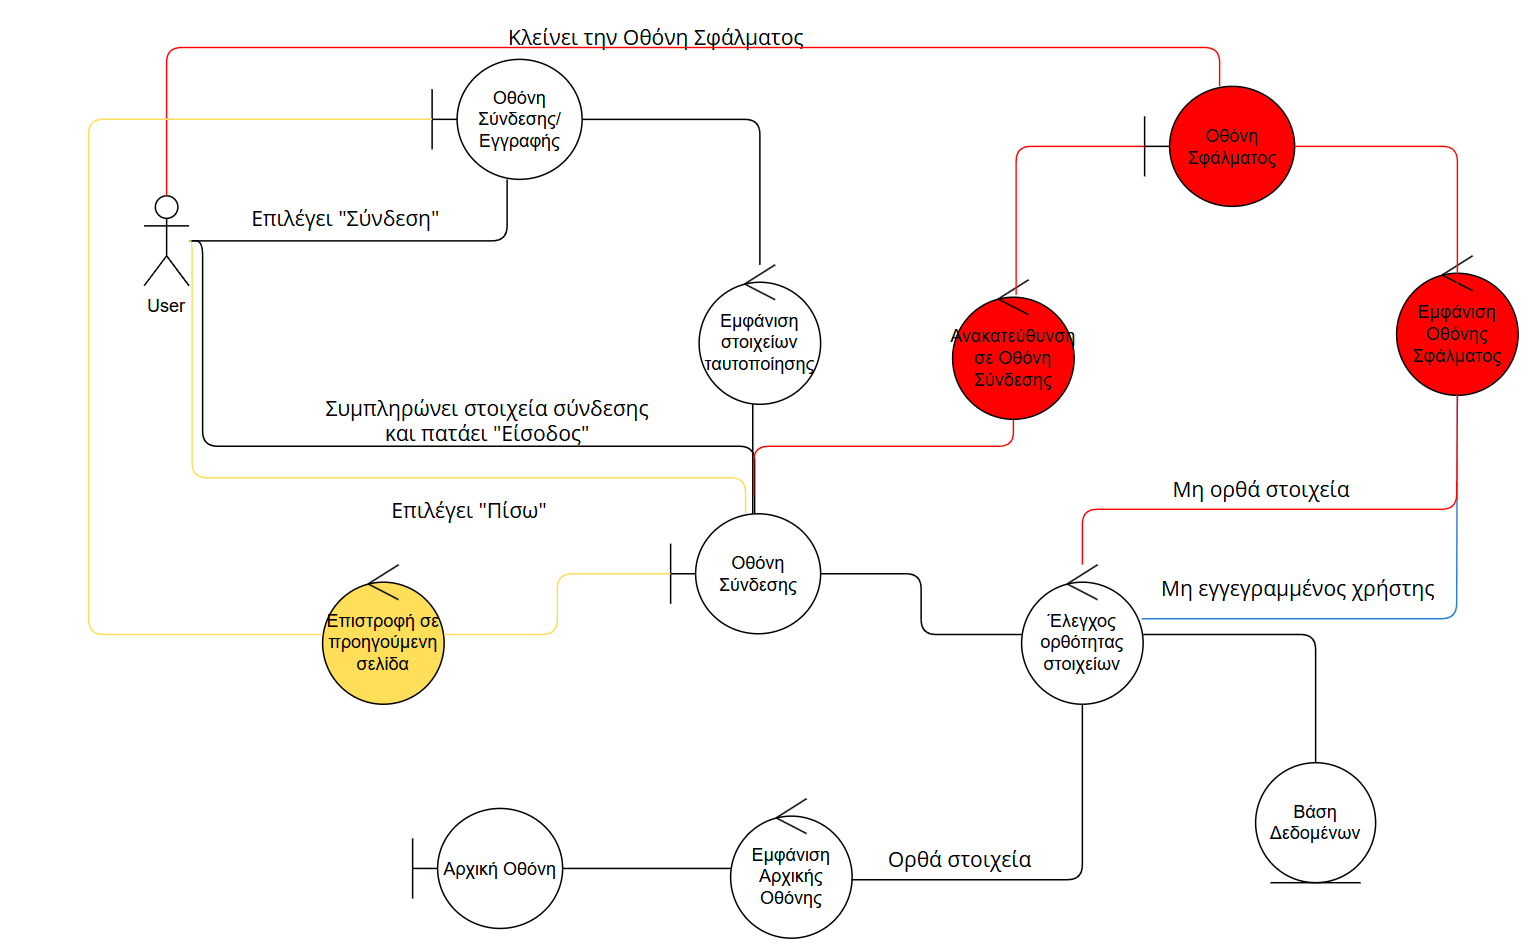
\includegraphics[width=0.8\textwidth]{Resources/Robustness Diagram/SignIn.png}
    \caption{User είναι Διαχειριστής, Γραμματέας, Κτηνίατρος, Pet Groomer και Πελάτης}\label{fig:robustness-signin}
\end{figure}

\subsection{Customer Management}
\begin{figure}[H]
    \centering
    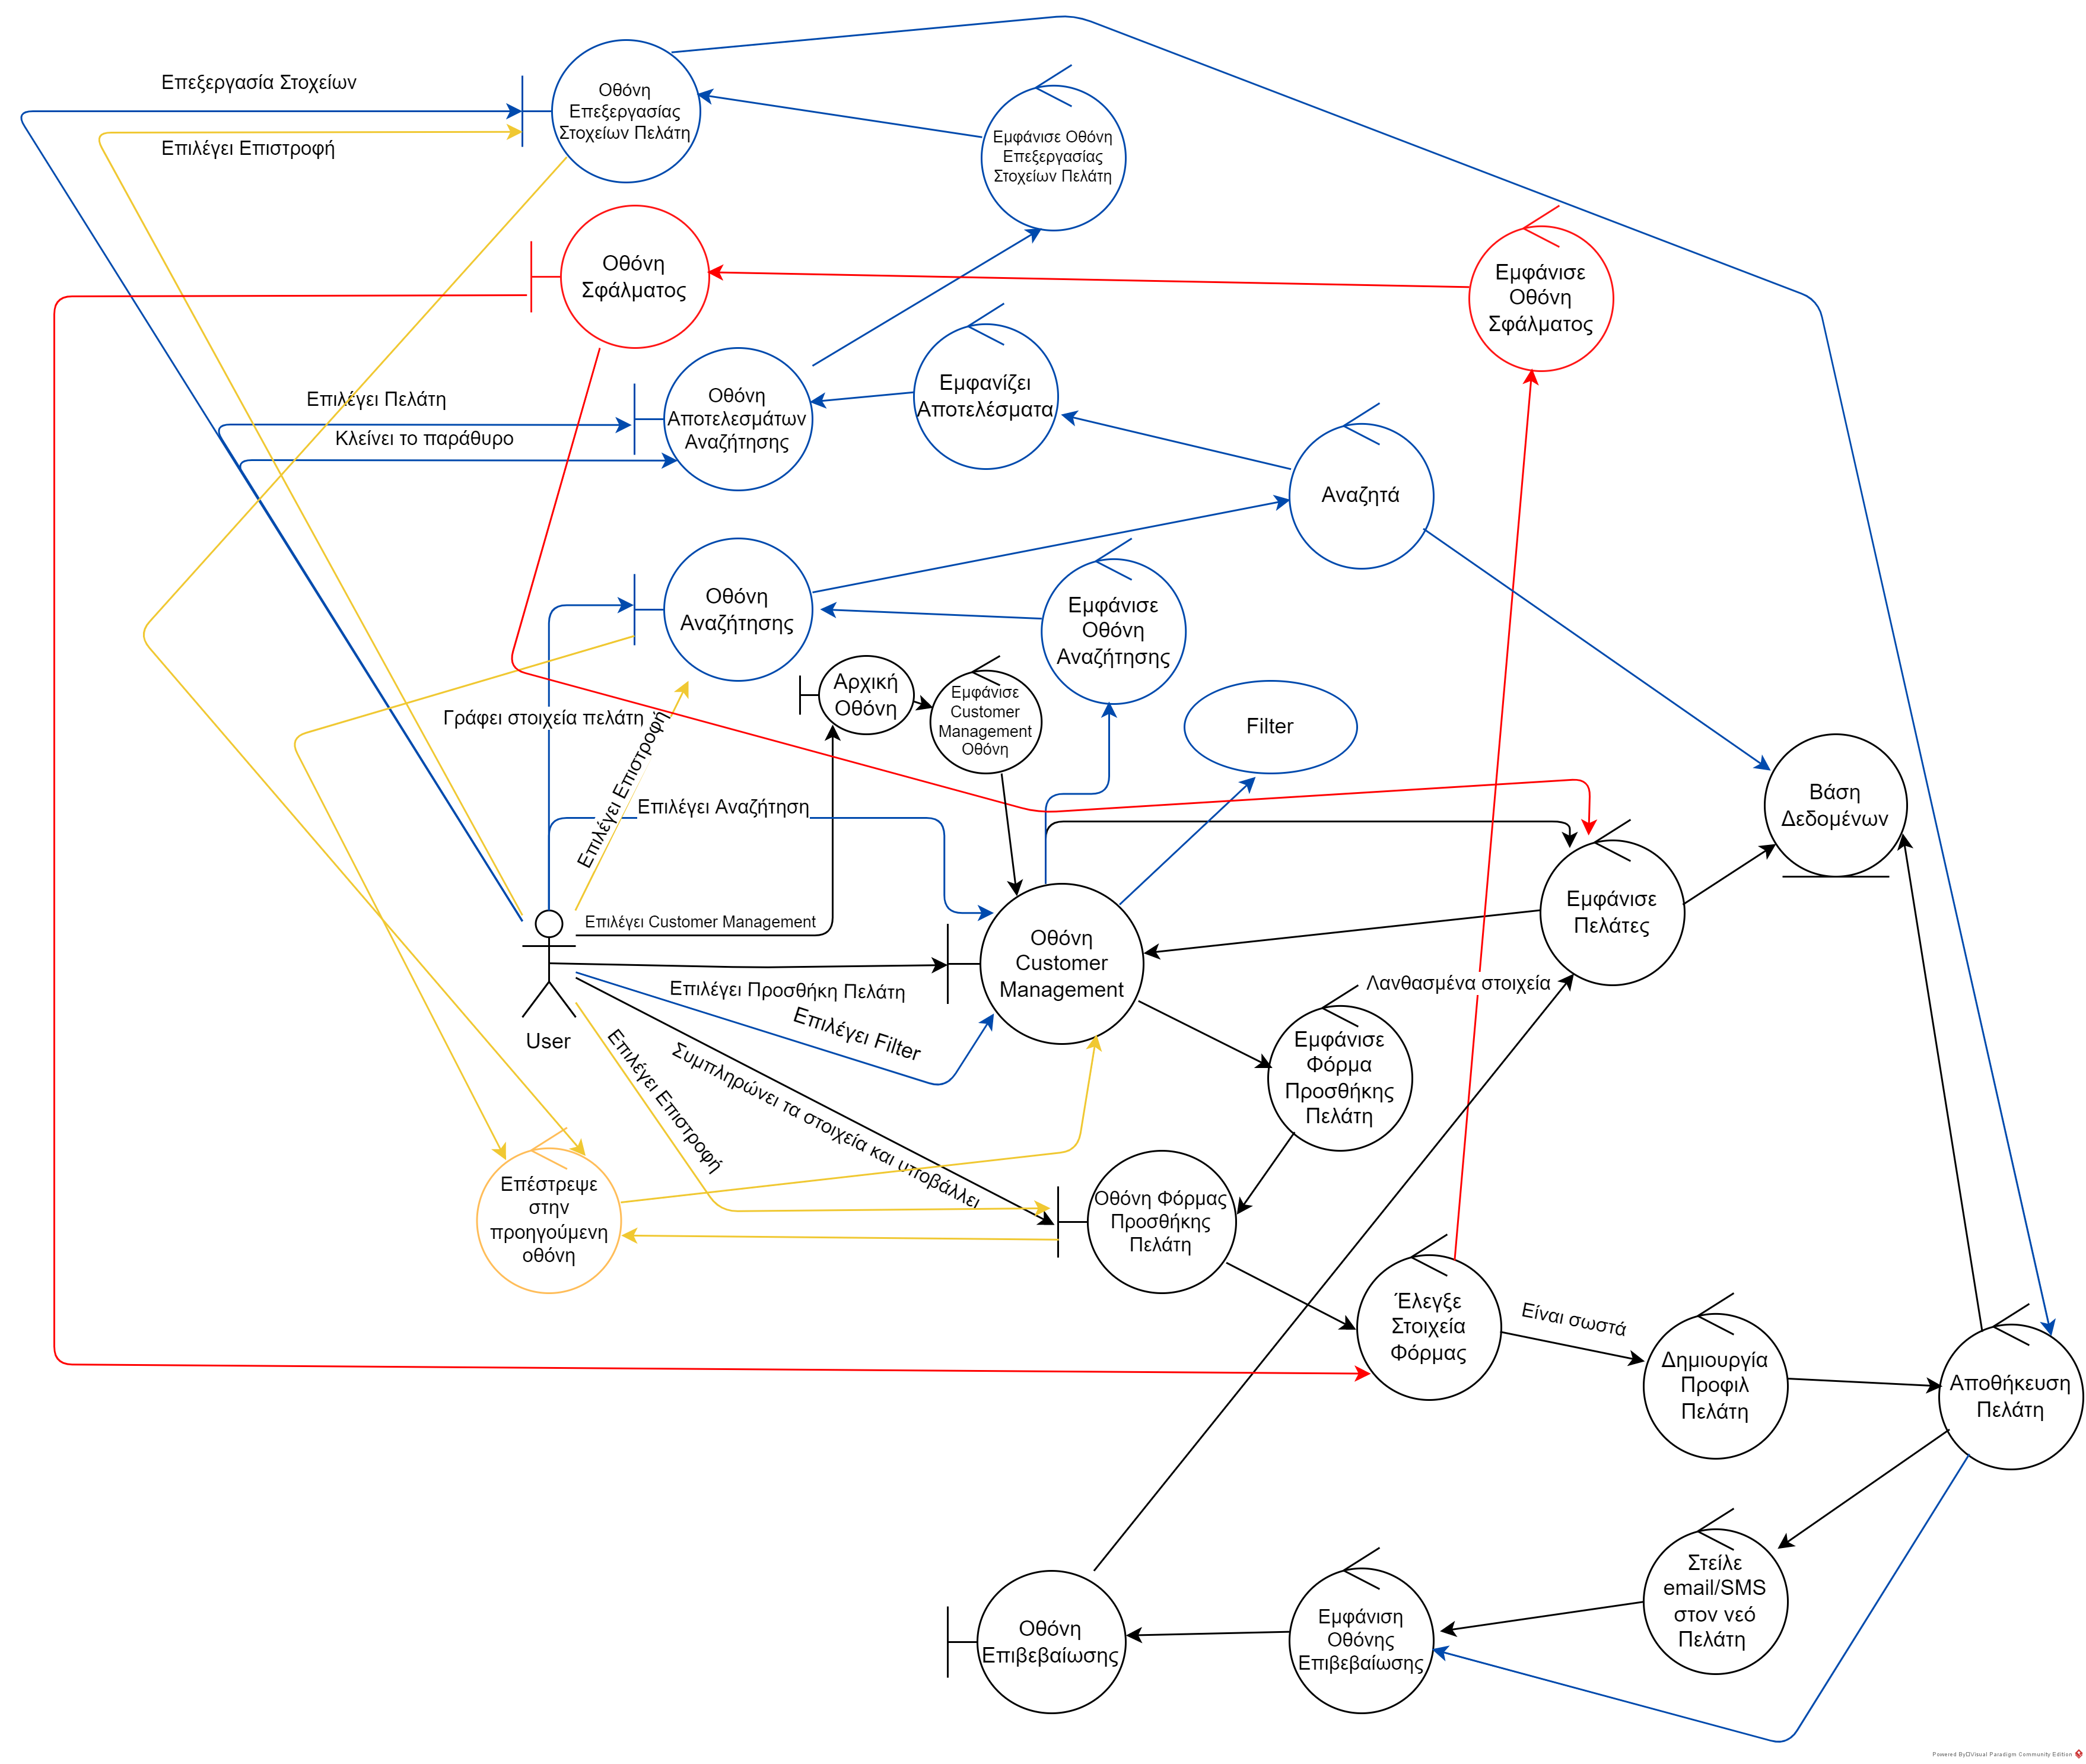
\includegraphics[width=0.8\textwidth]{Resources/Robustness Diagram/Customer_Management_RD.png}
    \caption{User είναι Διαχειριστής και Γραμματέας}\label{fig:robustness-customer-management}
\end{figure}

\subsection{Filter}
\begin{figure}[H]
    \centering
    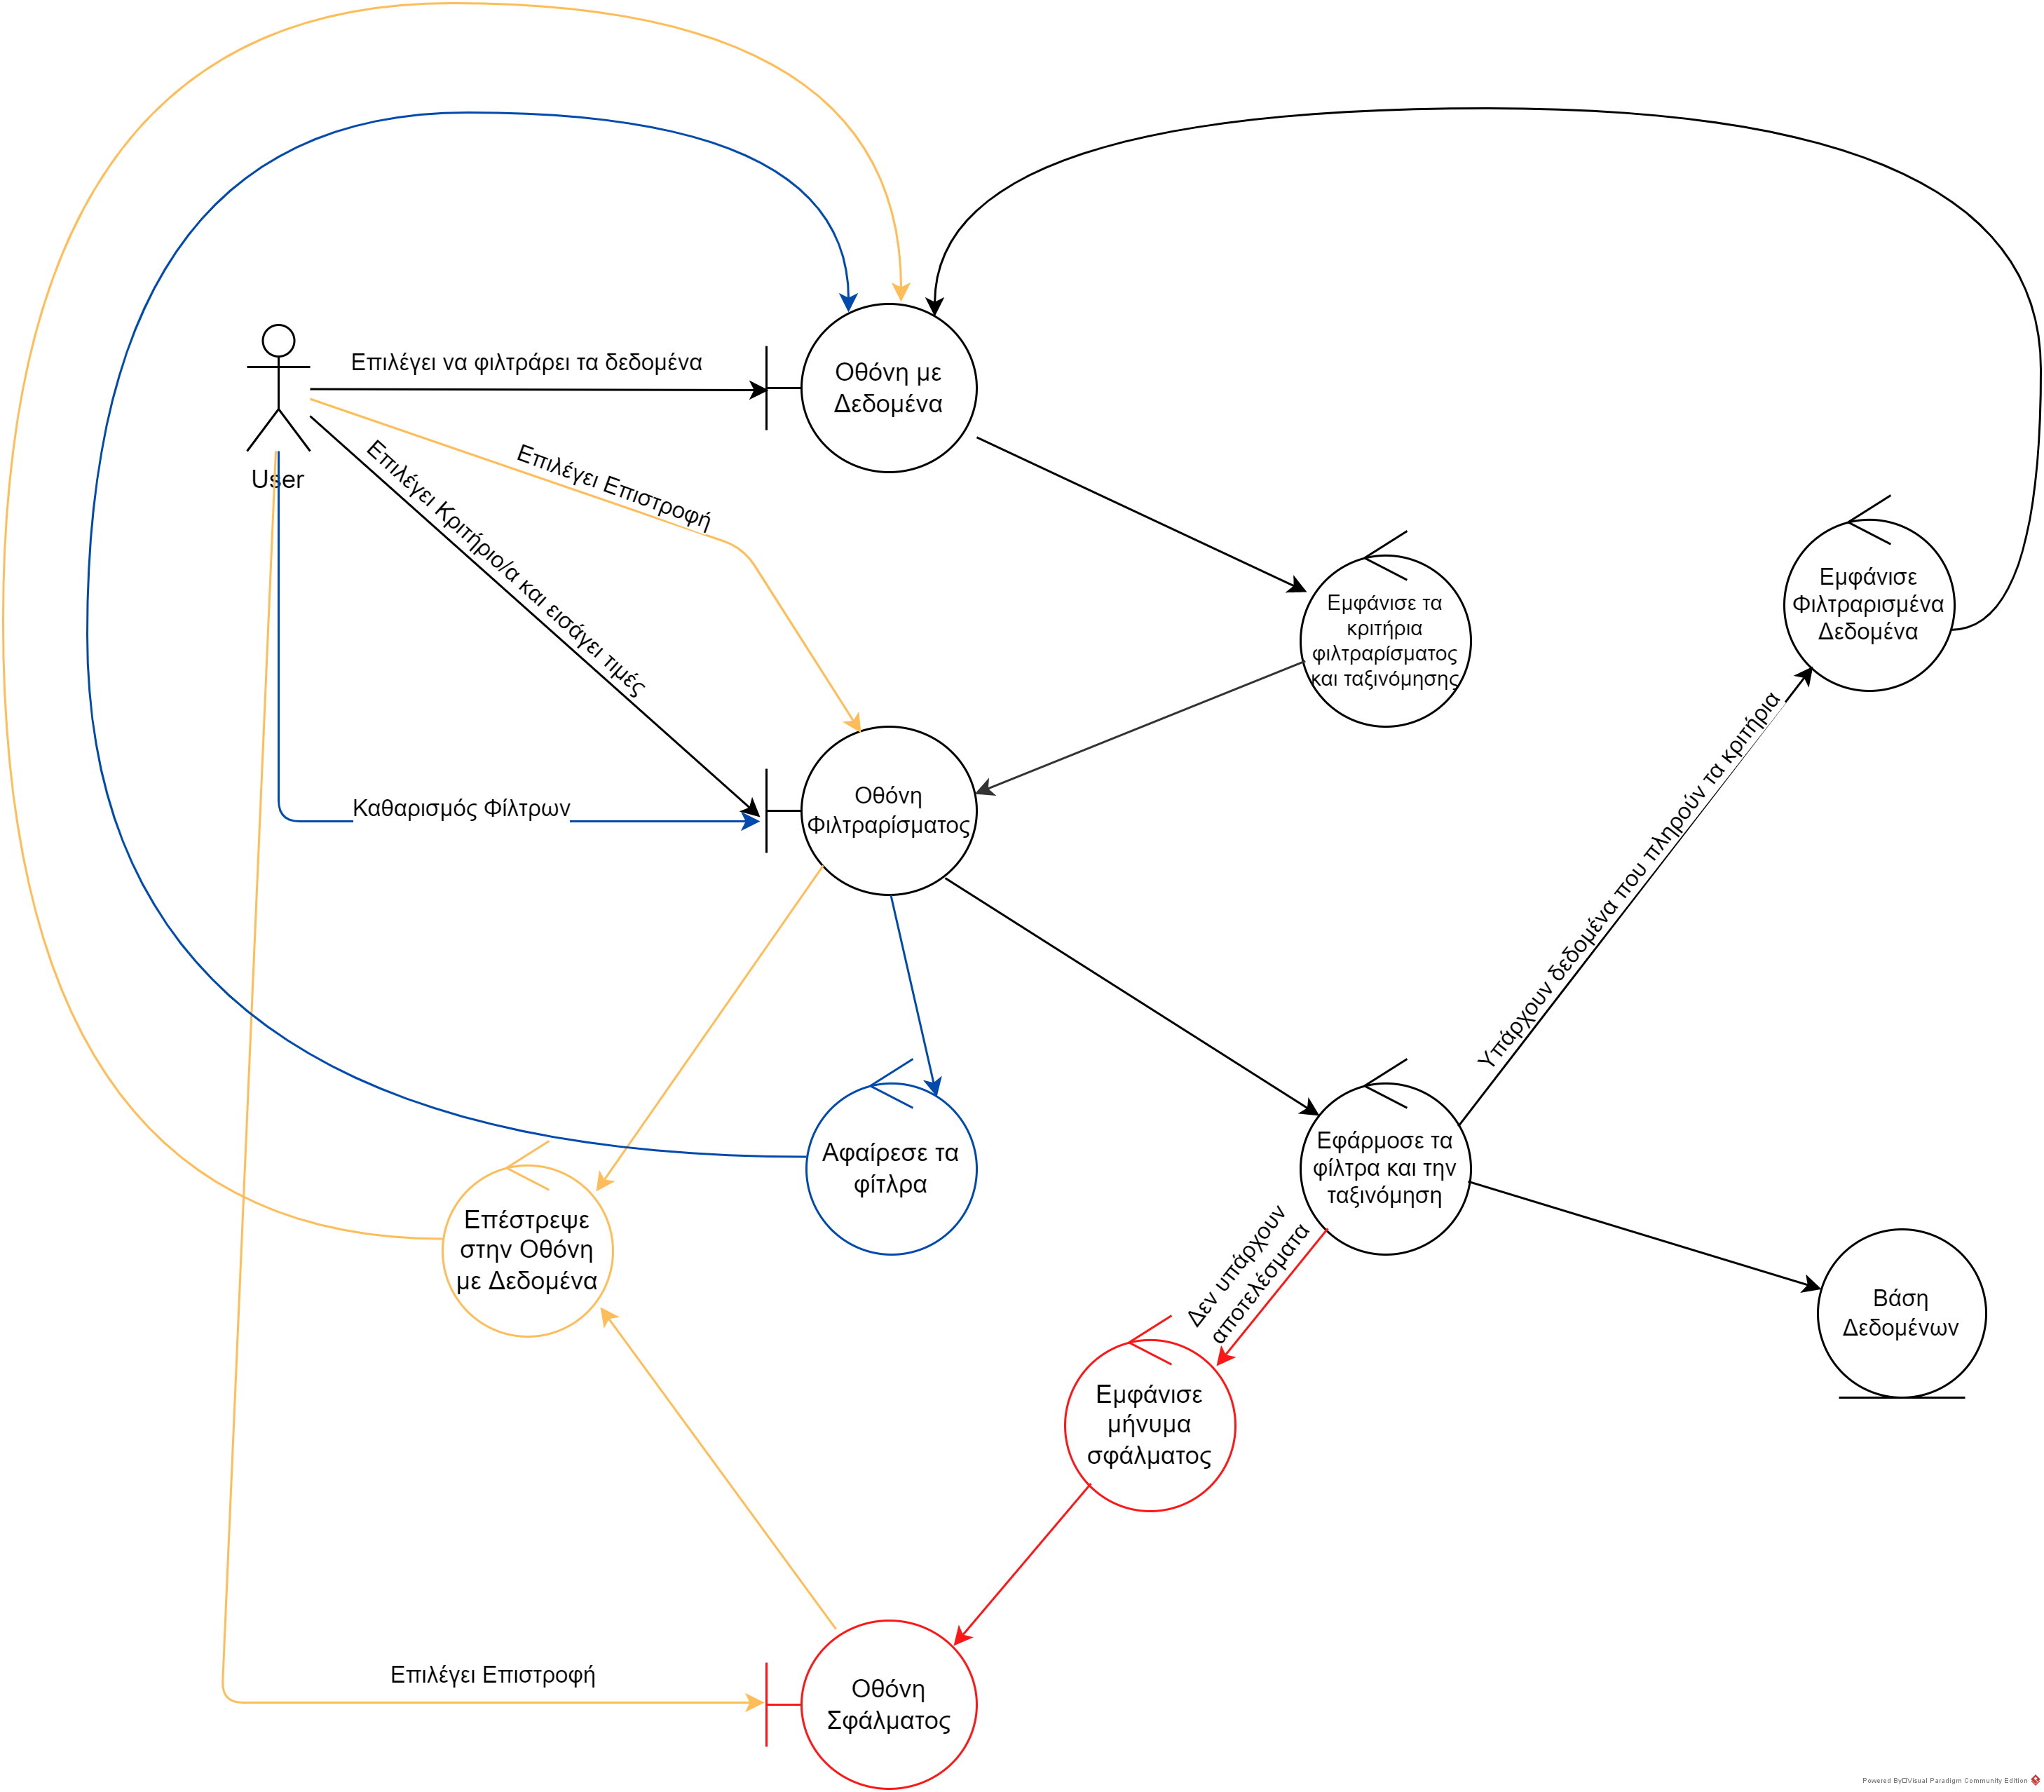
\includegraphics[width=\textwidth]{Resources/Robustness Diagram/Filter_RD.png}
    \caption{User είναι Διαχειριστής, Γραμματέας, Κτηνίατρος και Πελάτης}\label{fig:robustness-filter}
\end{figure}

\subsection{Warehouse Management}
\begin{figure}[H]
    \centering
    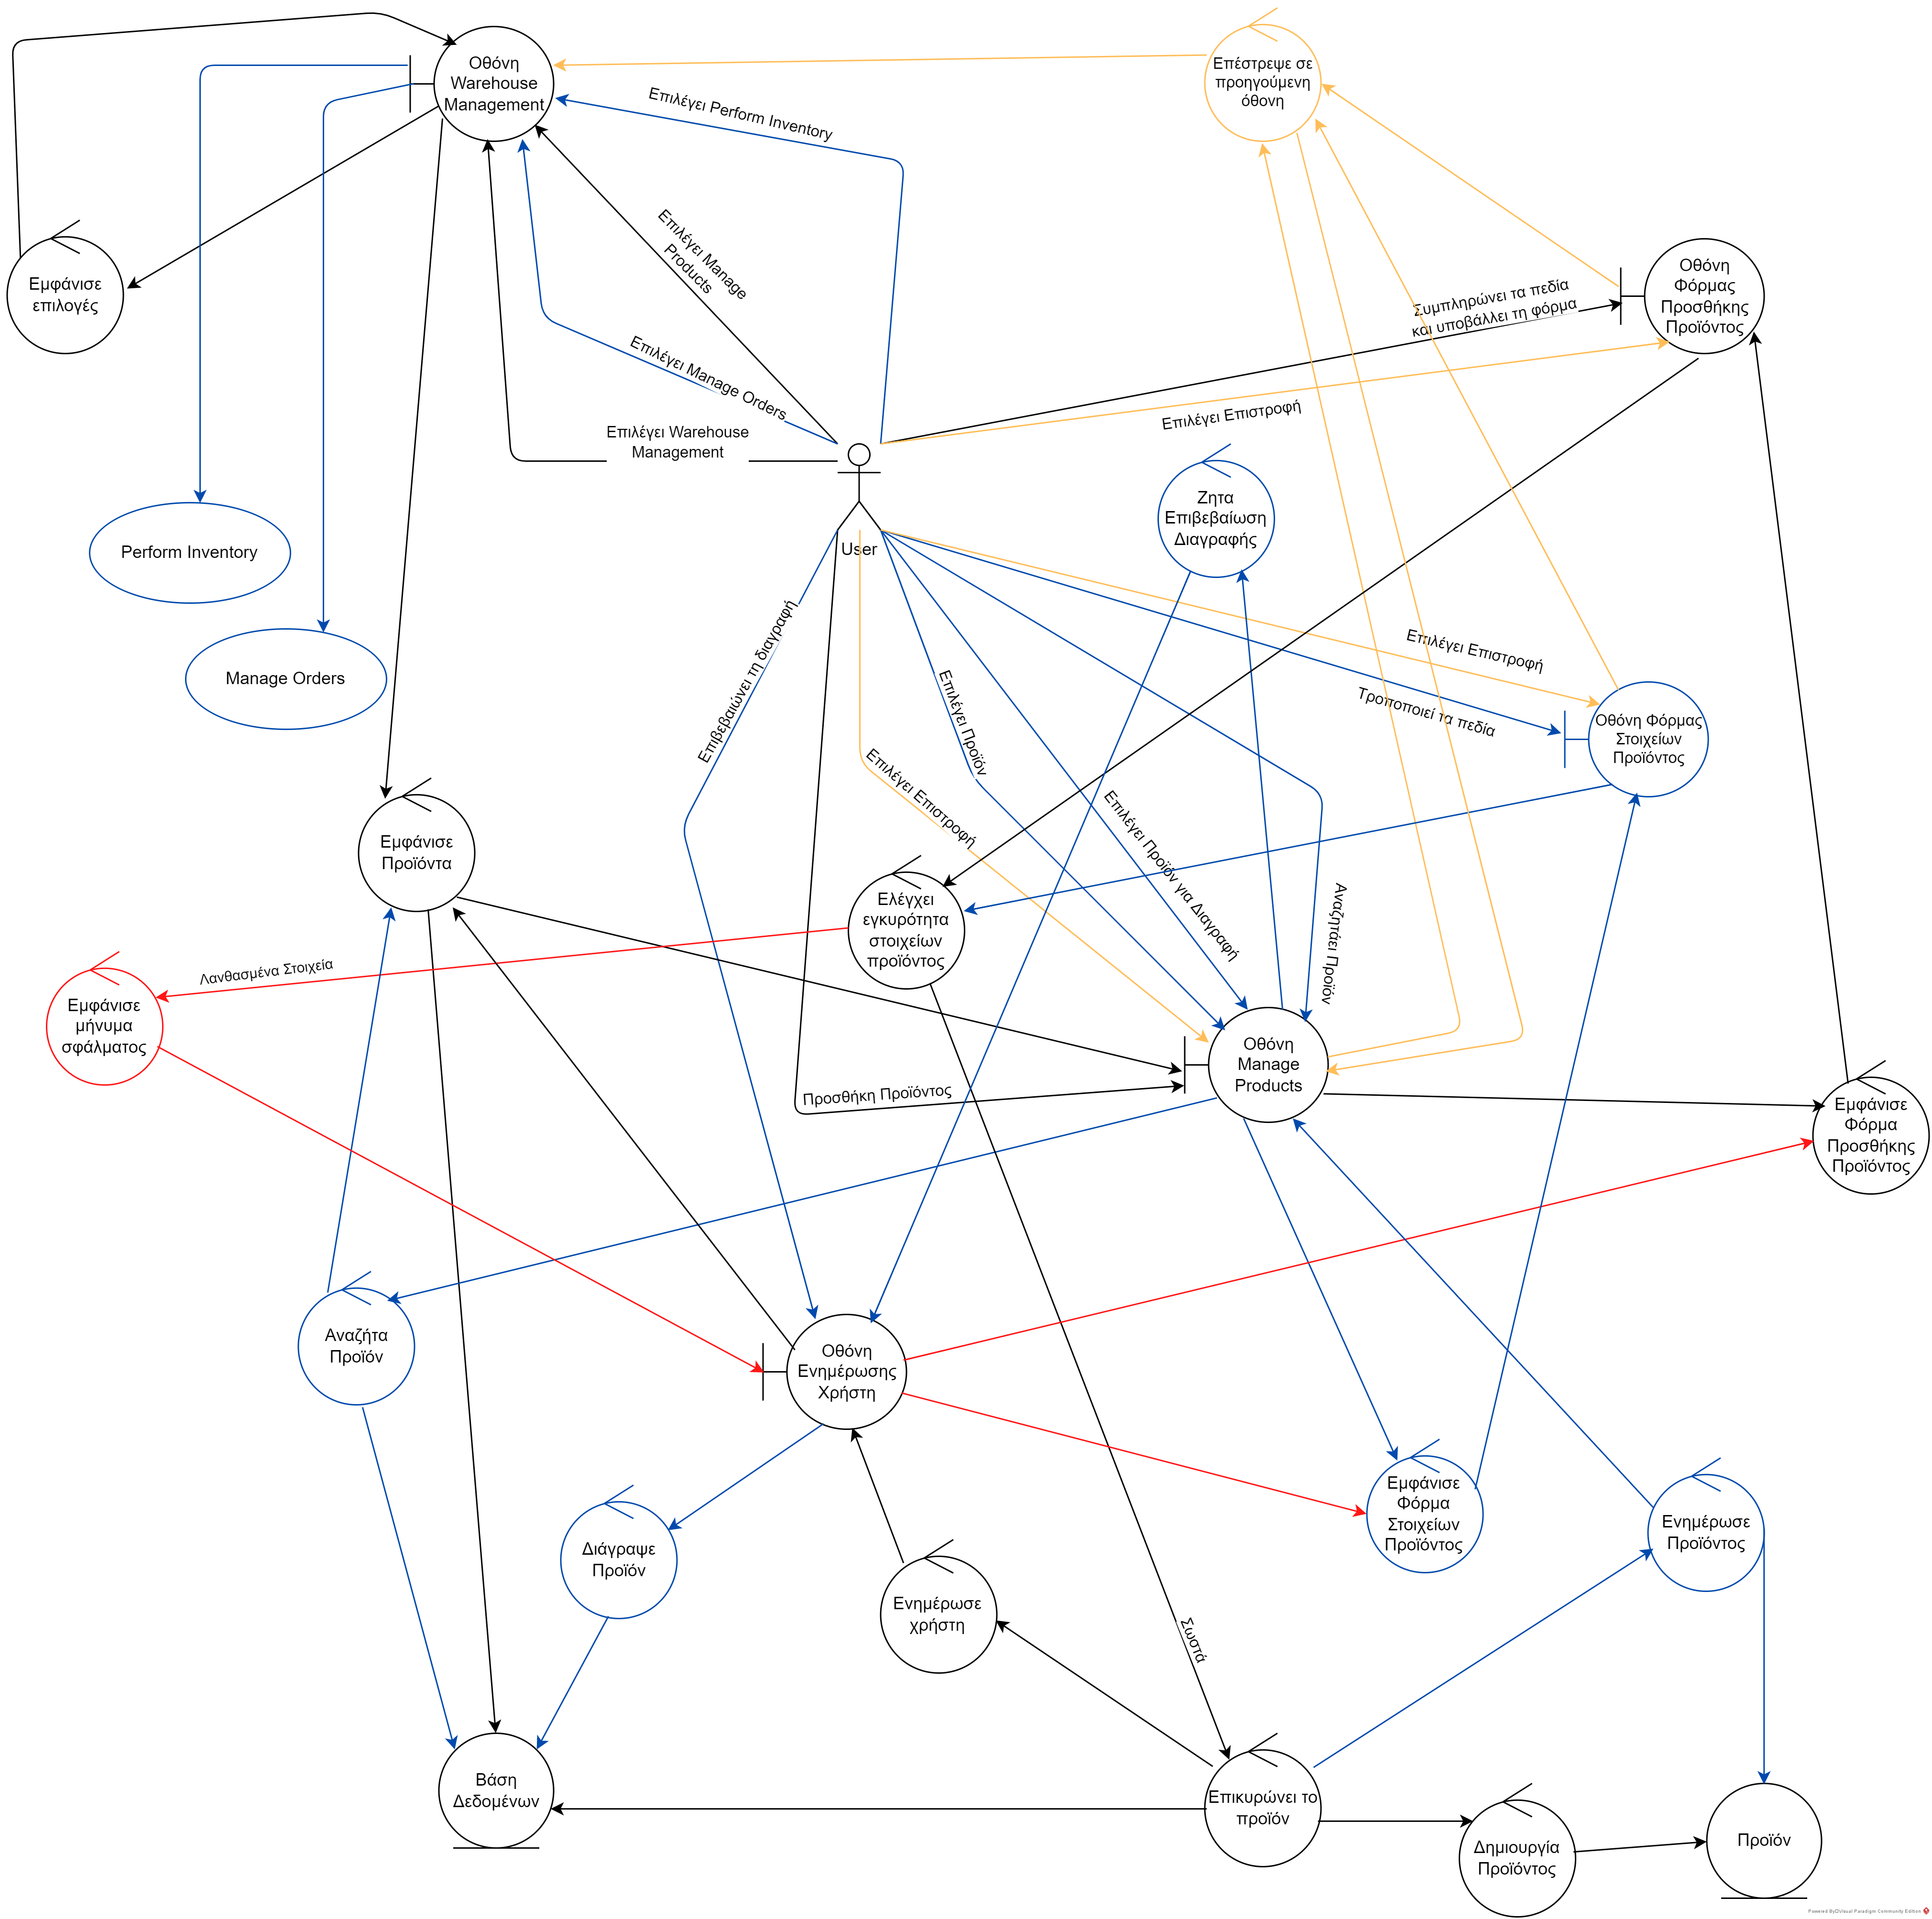
\includegraphics[width=\textwidth]{Resources/Robustness Diagram/Warehouse_Management_RD.png}
    \caption{User είναι Διαχειριστής, Κτηνίατρος και Γραμματέας}\label{fig:robustness-warehouse-management}
\end{figure}

\subsection{Perform Inventory}
\begin{figure}[H]
    \centering
    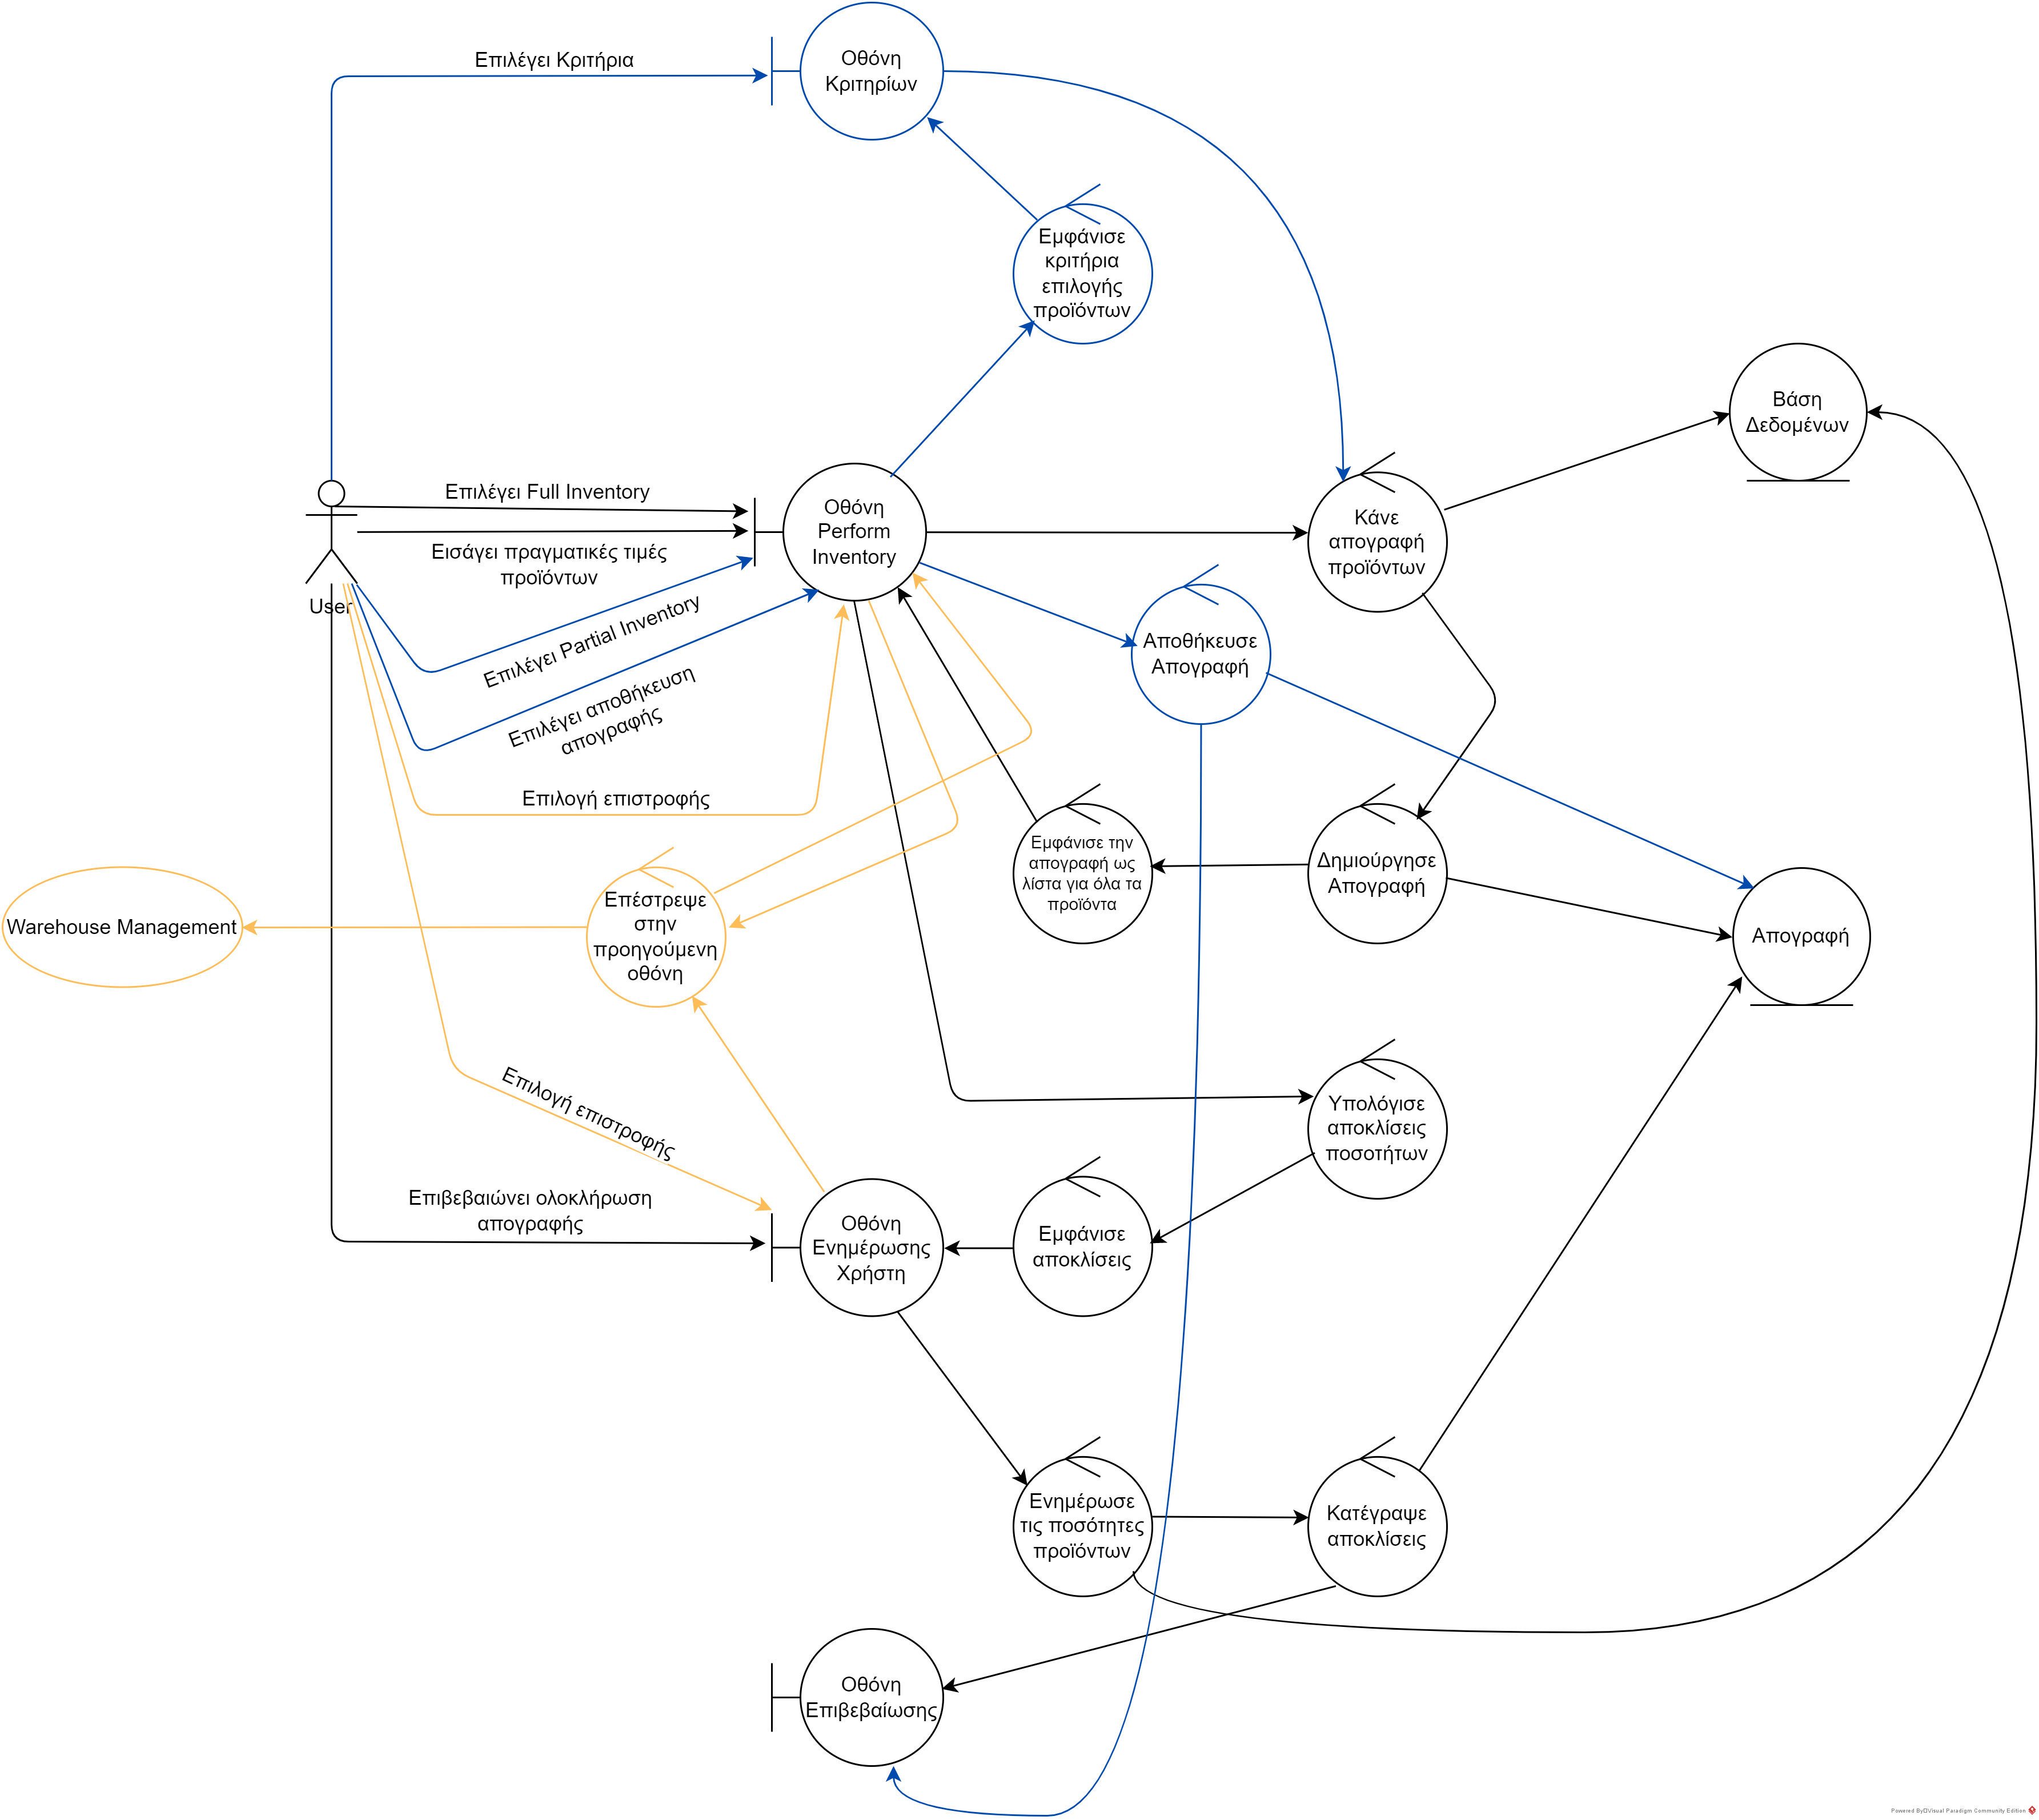
\includegraphics[width=\textwidth]{Resources/Robustness Diagram/Perform_Inventory_RD.png}
    \caption{User είναι Διαχειριστής, Κτηνίατρος και Γραμματέας}\label{fig:robustness-perform-inventory}
\end{figure}

\subsection{Manage Orders}
\begin{figure}[H]
    \centering
    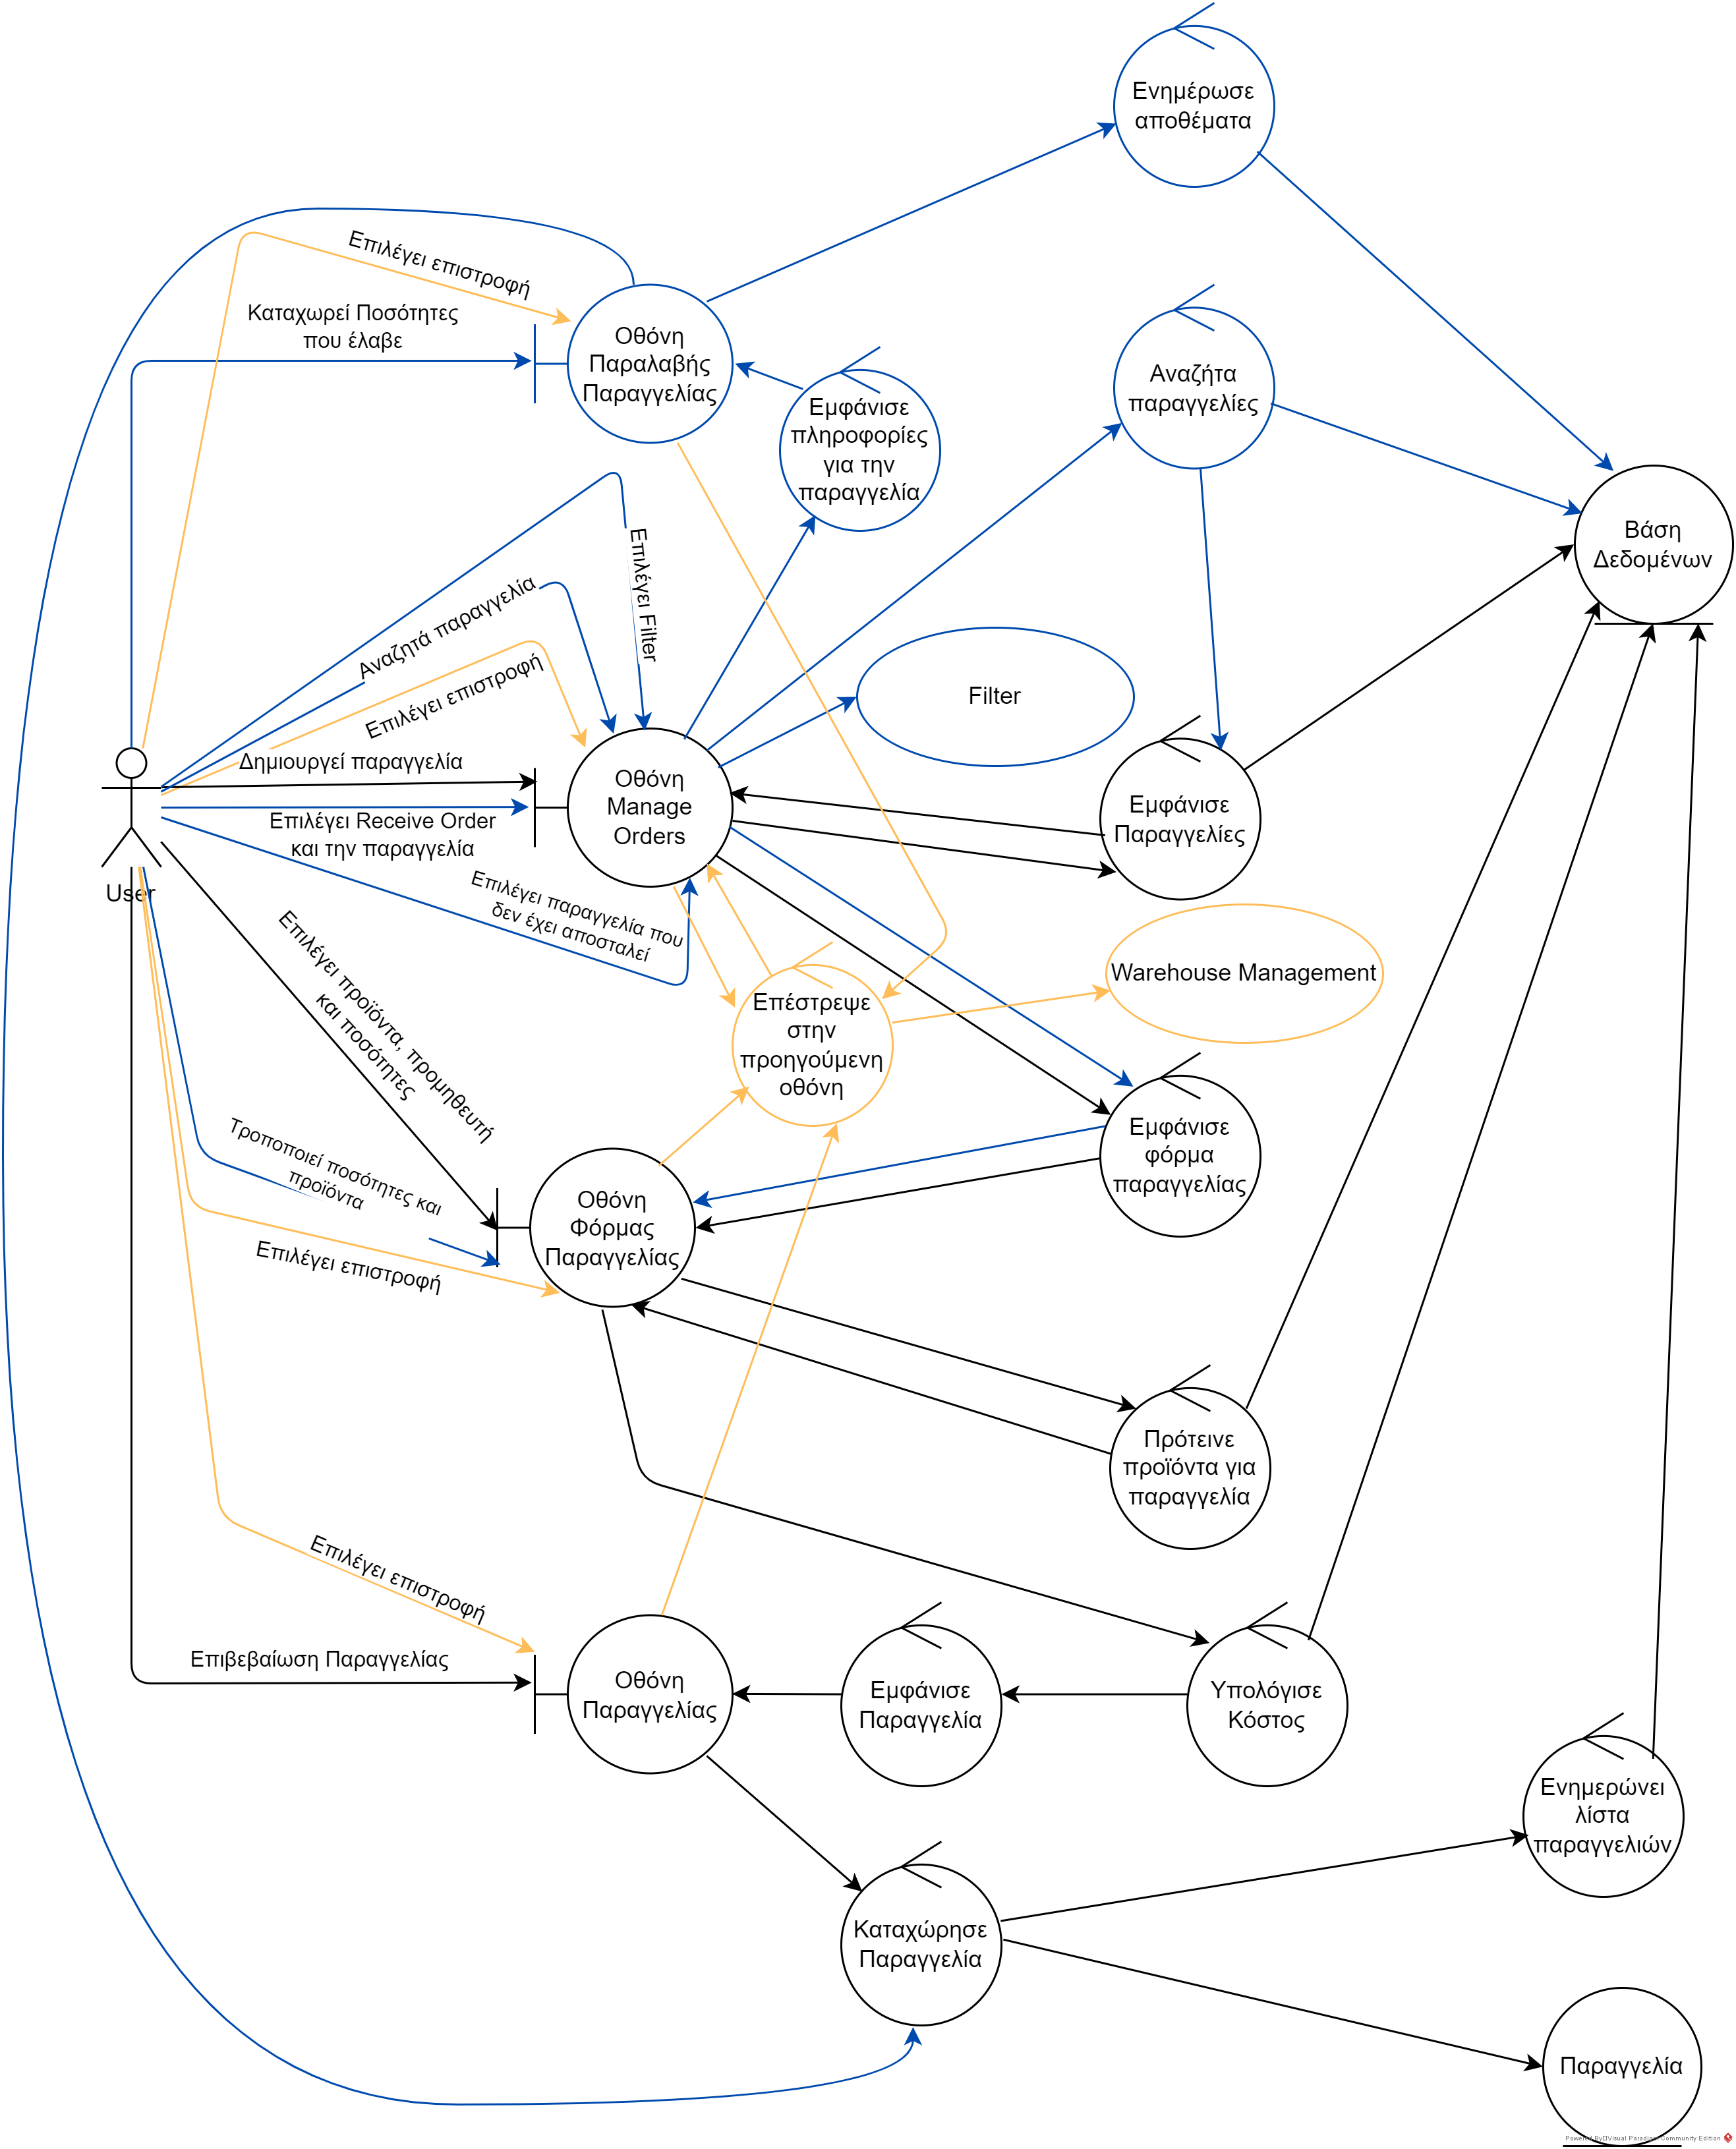
\includegraphics[width=\textwidth]{Resources/Robustness Diagram/Manage_Orders_RD.png}
    \caption{User είναι Διαχειριστής, Κτηνίατρος και Γραμματέας}\label{fig:robustness-manage-orders}
\end{figure}

\subsection{Store}
\begin{figure}[H]
    \centering
    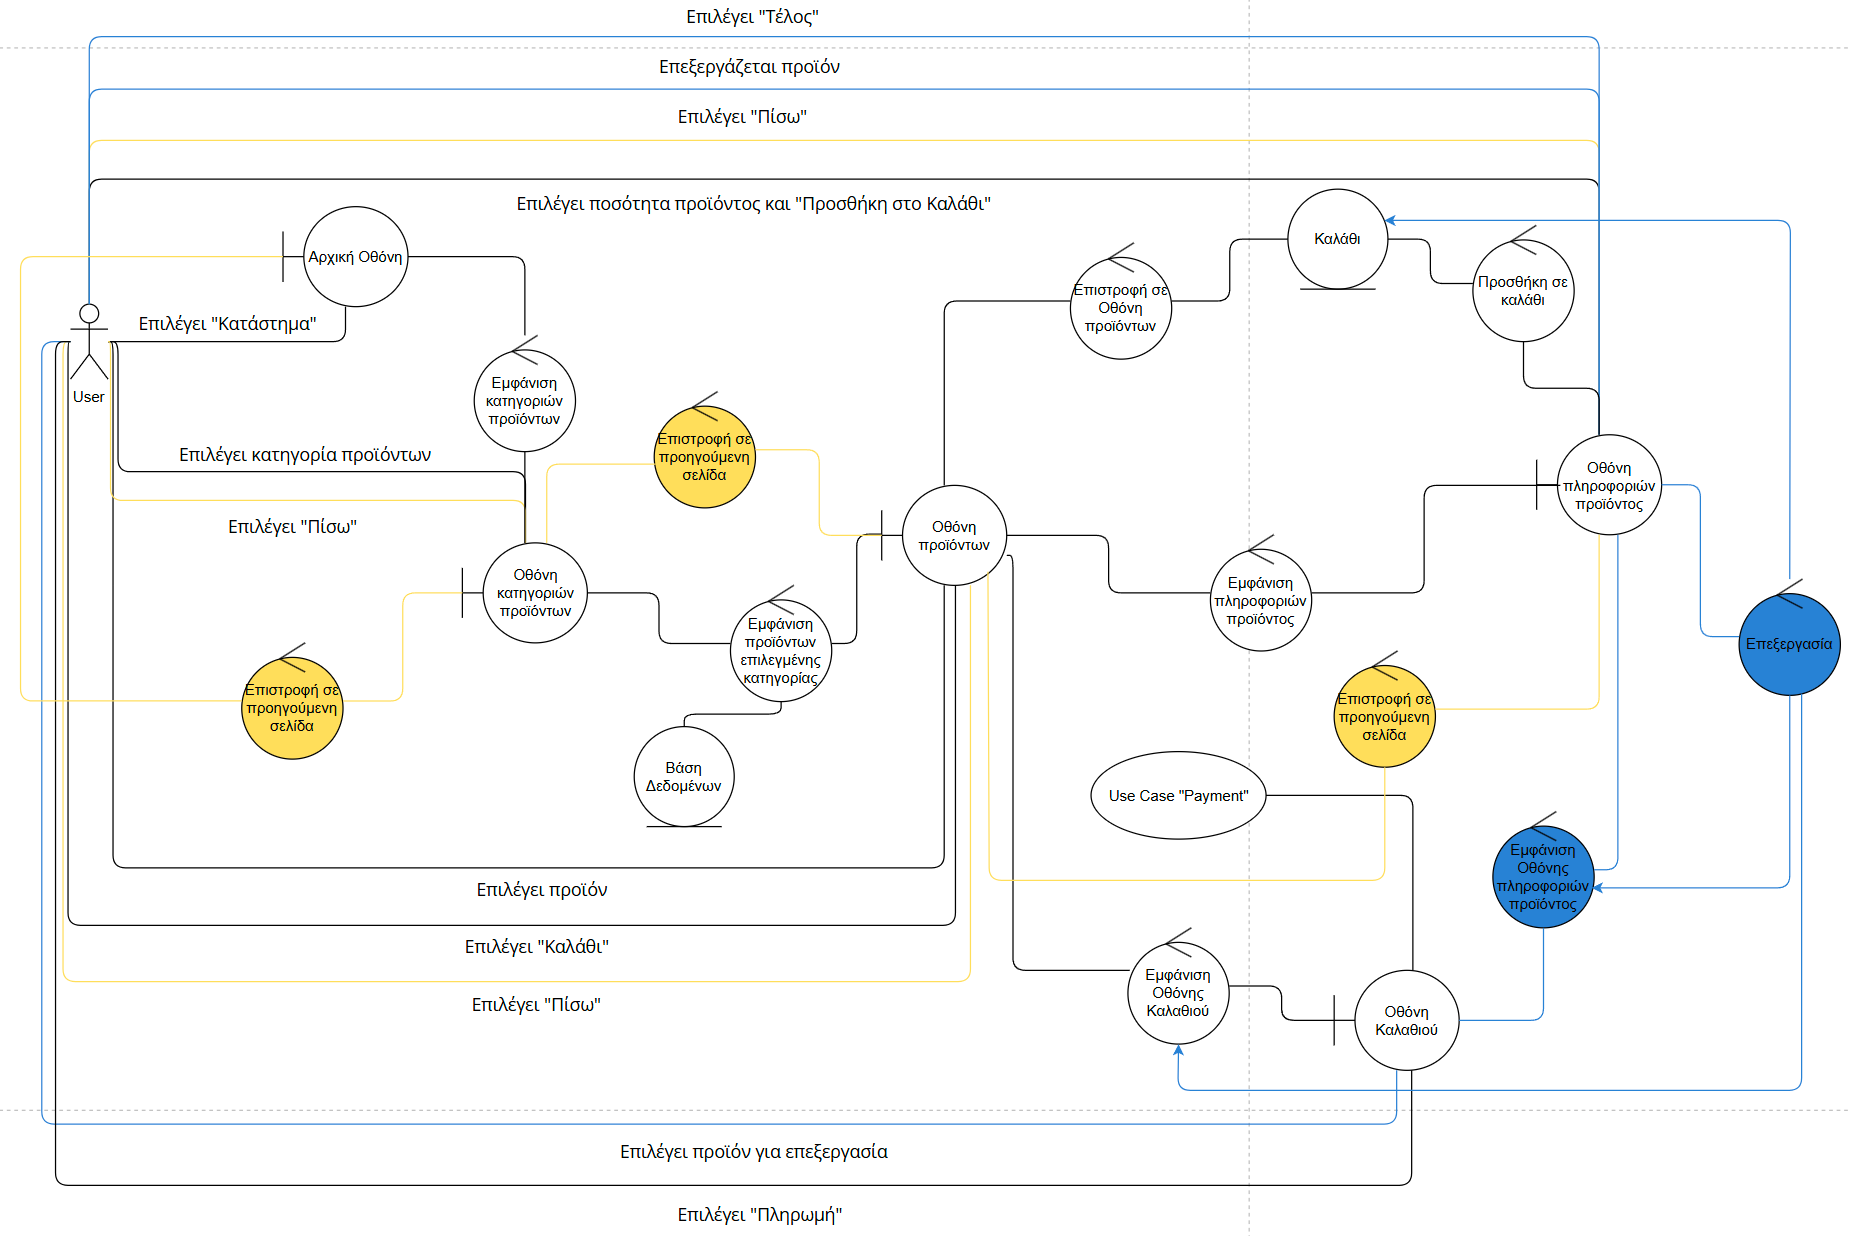
\includegraphics[width=0.8\textwidth]{Resources/Robustness Diagram/Store.png}
    \caption{User είναι Διαχειριστής και Πελάτης}\label{fig:robustness-store}
\end{figure}

\subsection{Payment}
\begin{figure}[H]
    \centering
    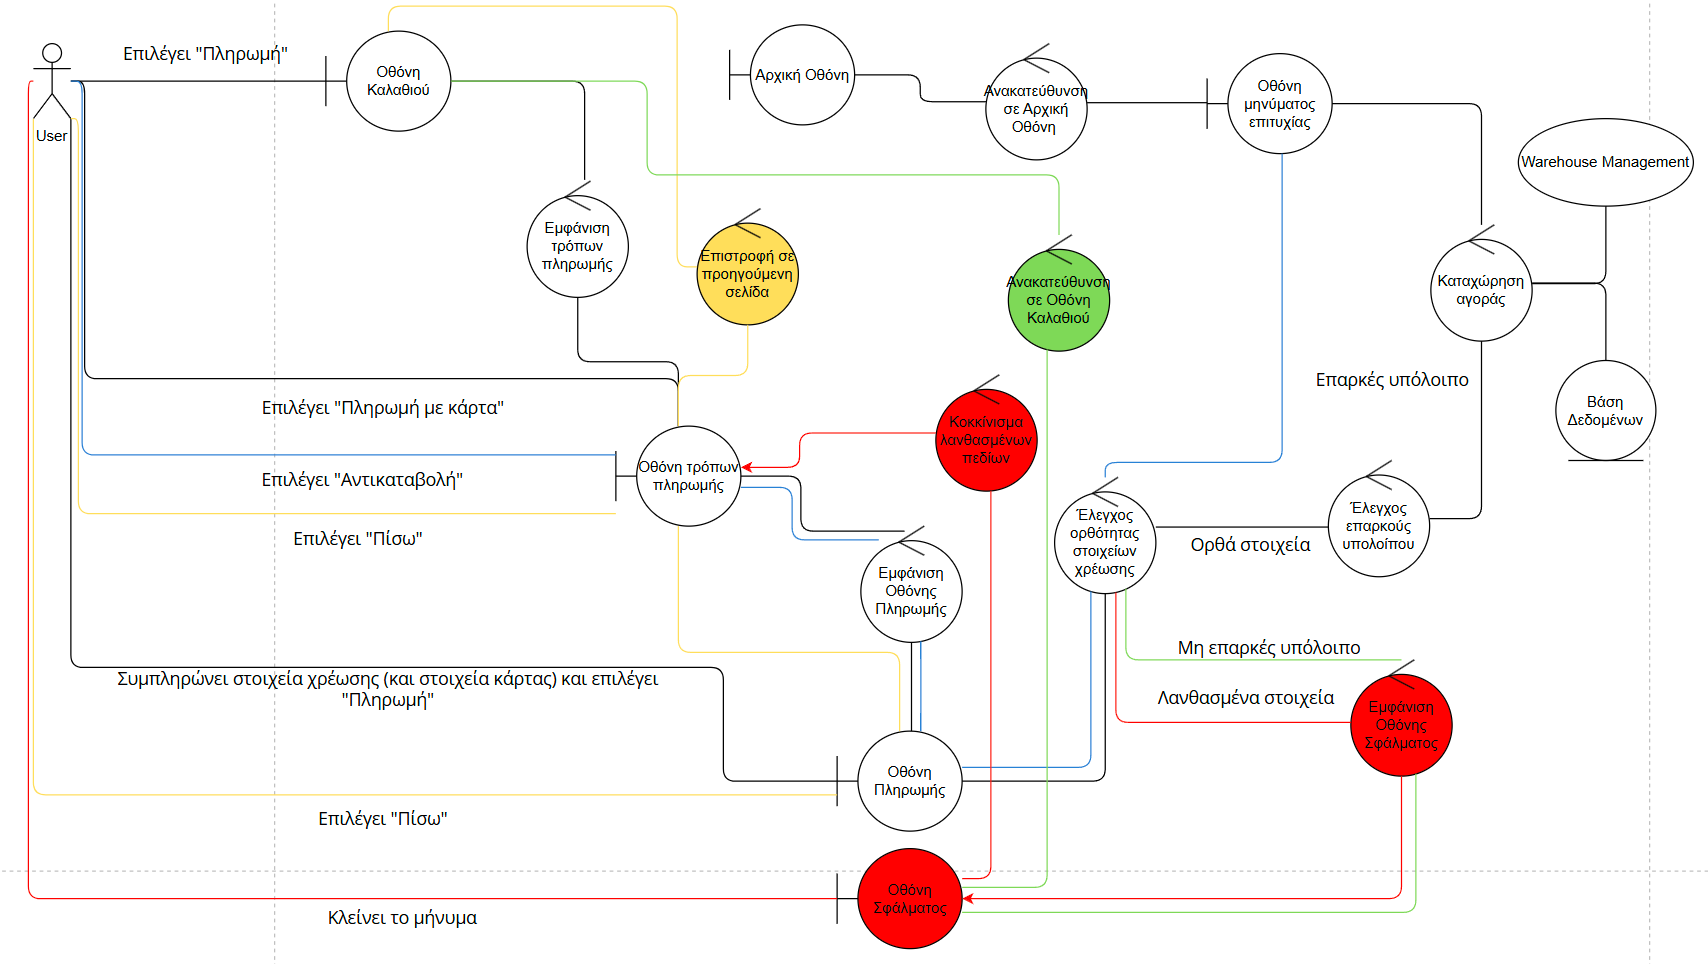
\includegraphics[width=0.8\textwidth]{Resources/Robustness Diagram/Payment.png}
    \caption{User είναι Διαχειριστής και Πελάτης}\label{fig:robustness-payment}
\end{figure}

\subsection{Appointment Management}
\begin{figure}[H]
    \centering
    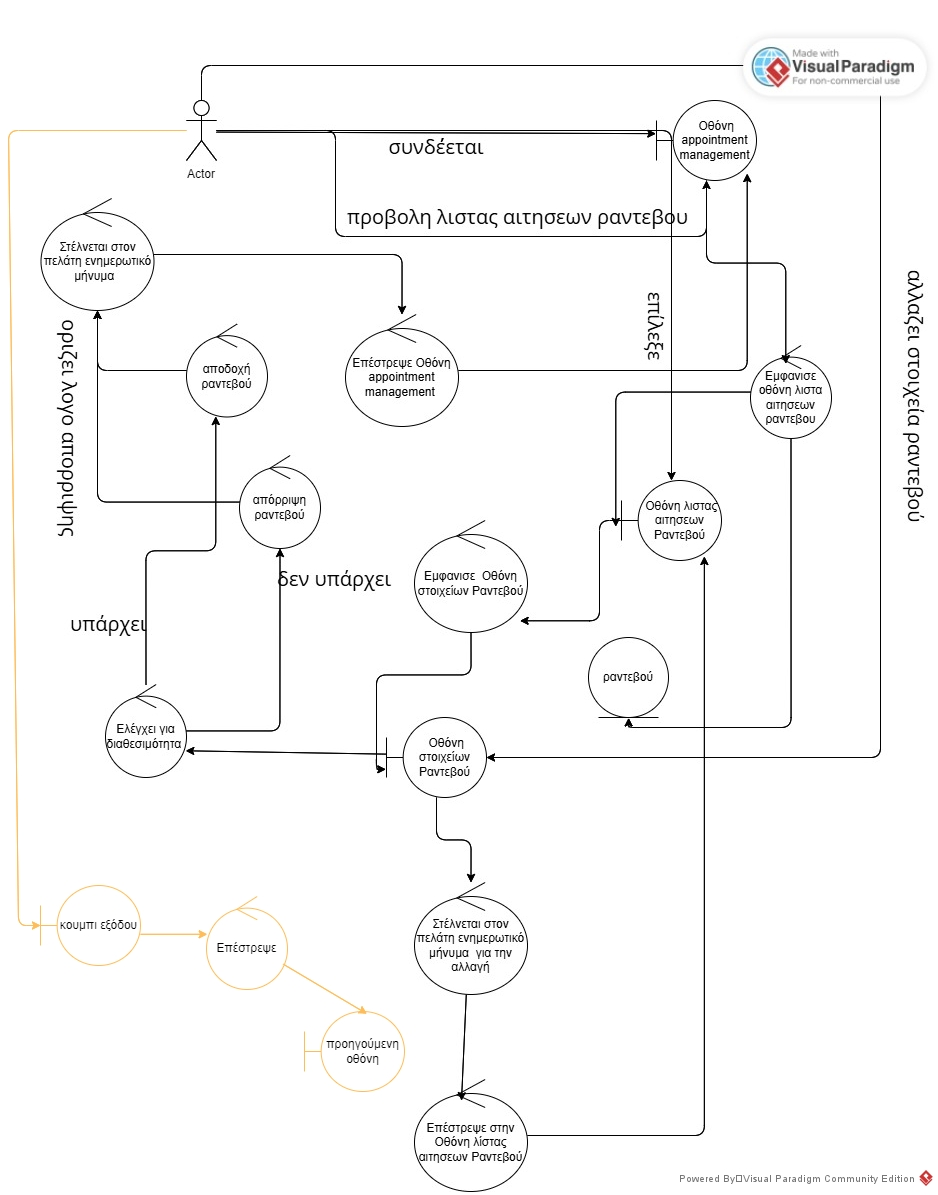
\includegraphics[width=\textwidth]{Resources/Robustness Diagram/appointment-management.jpg}
    \caption{Actor είναι Διαχειριστής, Γραμματέας, Pet Groomer και Κτηνίατρος}\label{fig:robustness-appointment-management}
\end{figure}

\subsection{Appointment Scheduling}
\begin{figure}[H]
    \centering
    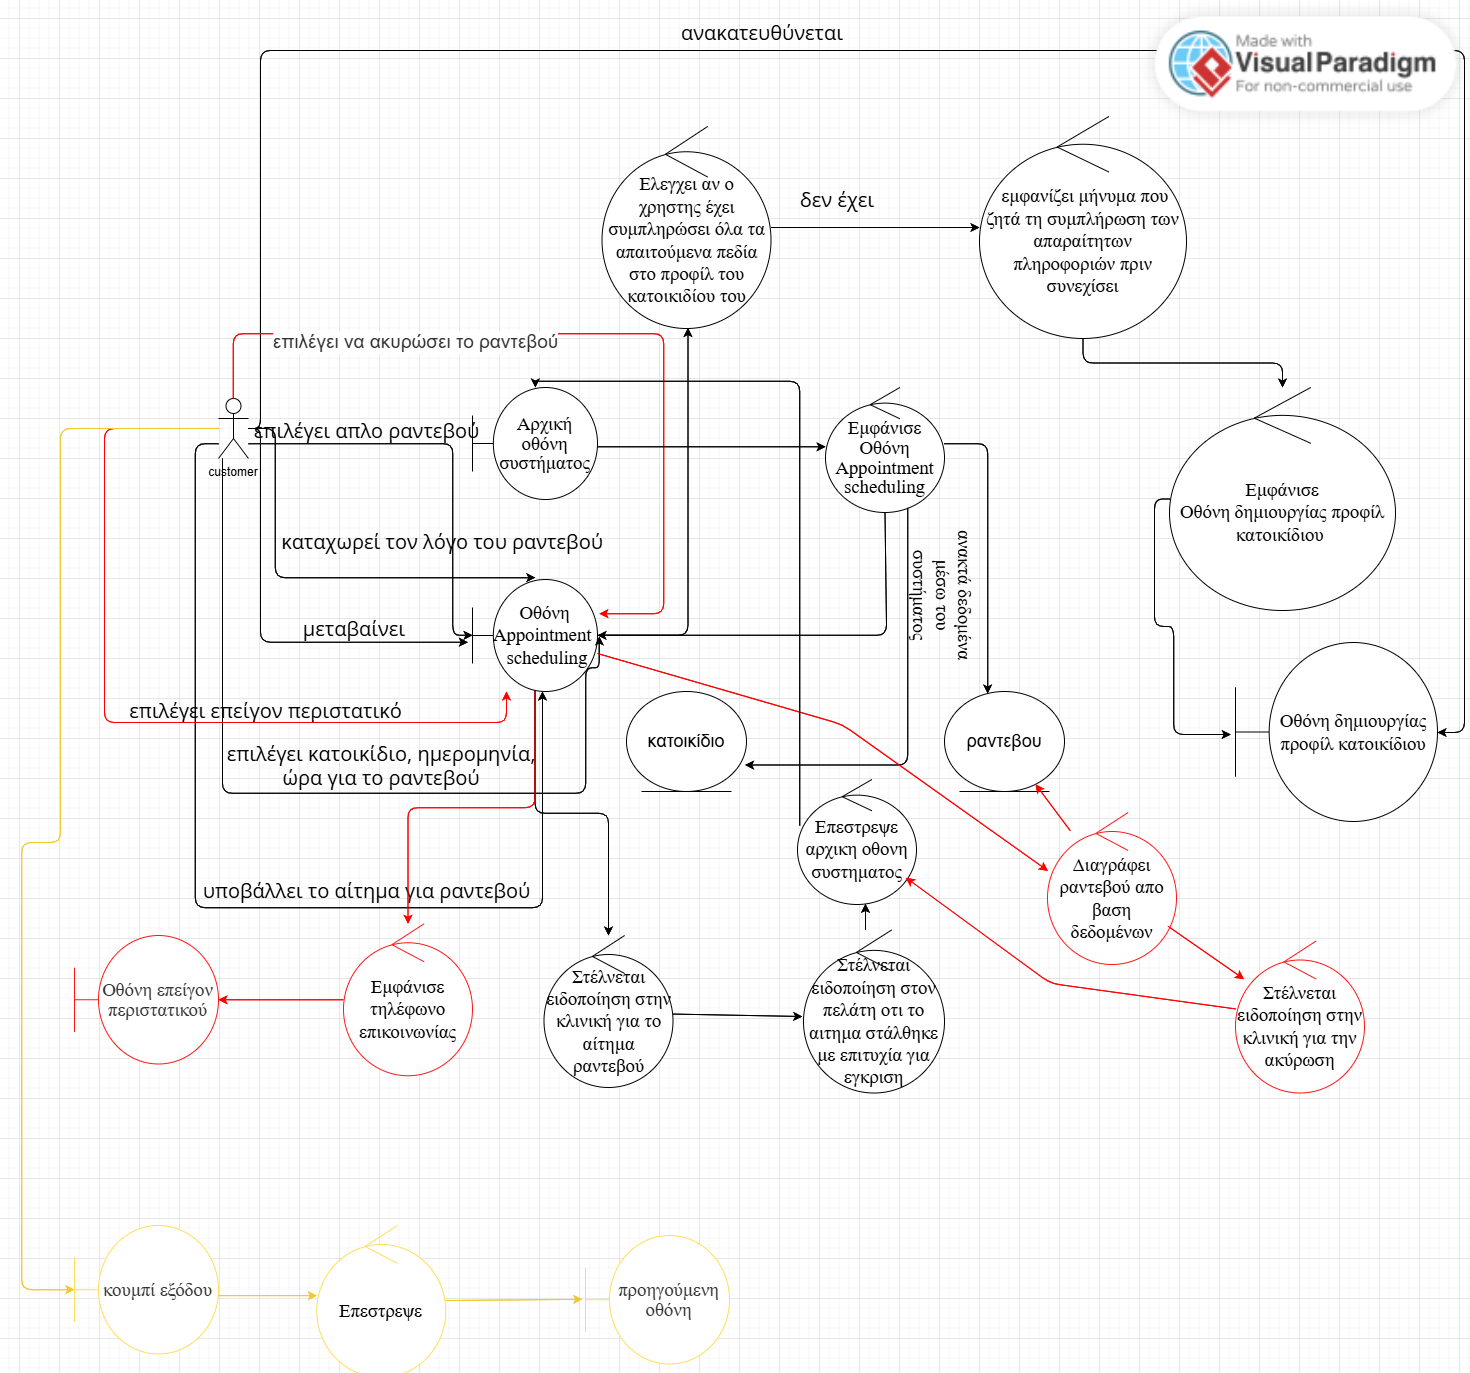
\includegraphics[width=\textwidth]{Resources/Robustness Diagram/appointment-scheduling.png}\label{fig:robustness-appointment-scheduling}
\end{figure}

\subsection{MedicalRecord}
\begin{figure}[H]
    \centering
    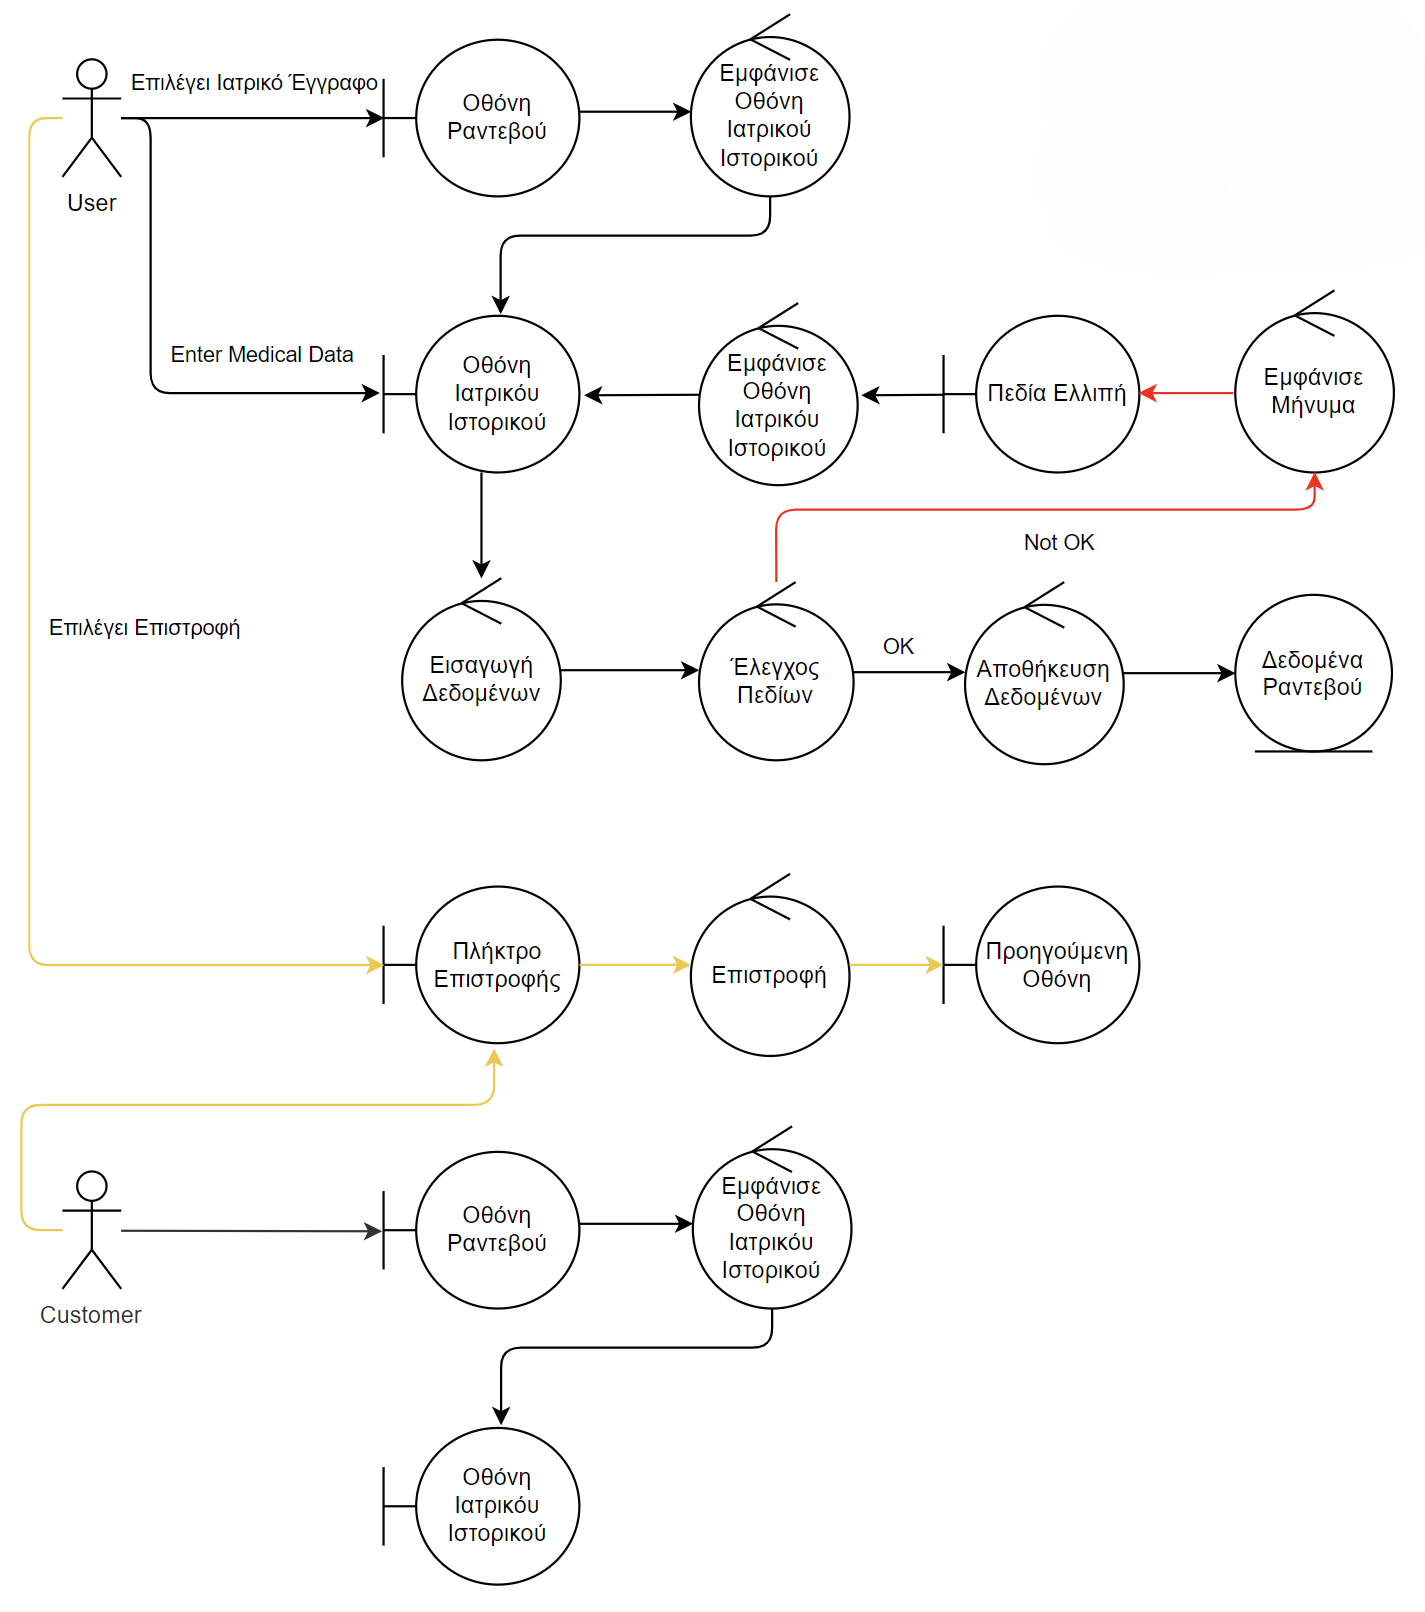
\includegraphics[width=\textwidth]{Resources/Robustness Diagram/Medical_Record.png}
    \caption{User είναι Διαχειριστής, Πελάτης και Κτηνίατρος}\label{fig:robustness-medical-record}
\end{figure}

\subsection{Subscriptions}
\begin{figure}[H]
    \centering
    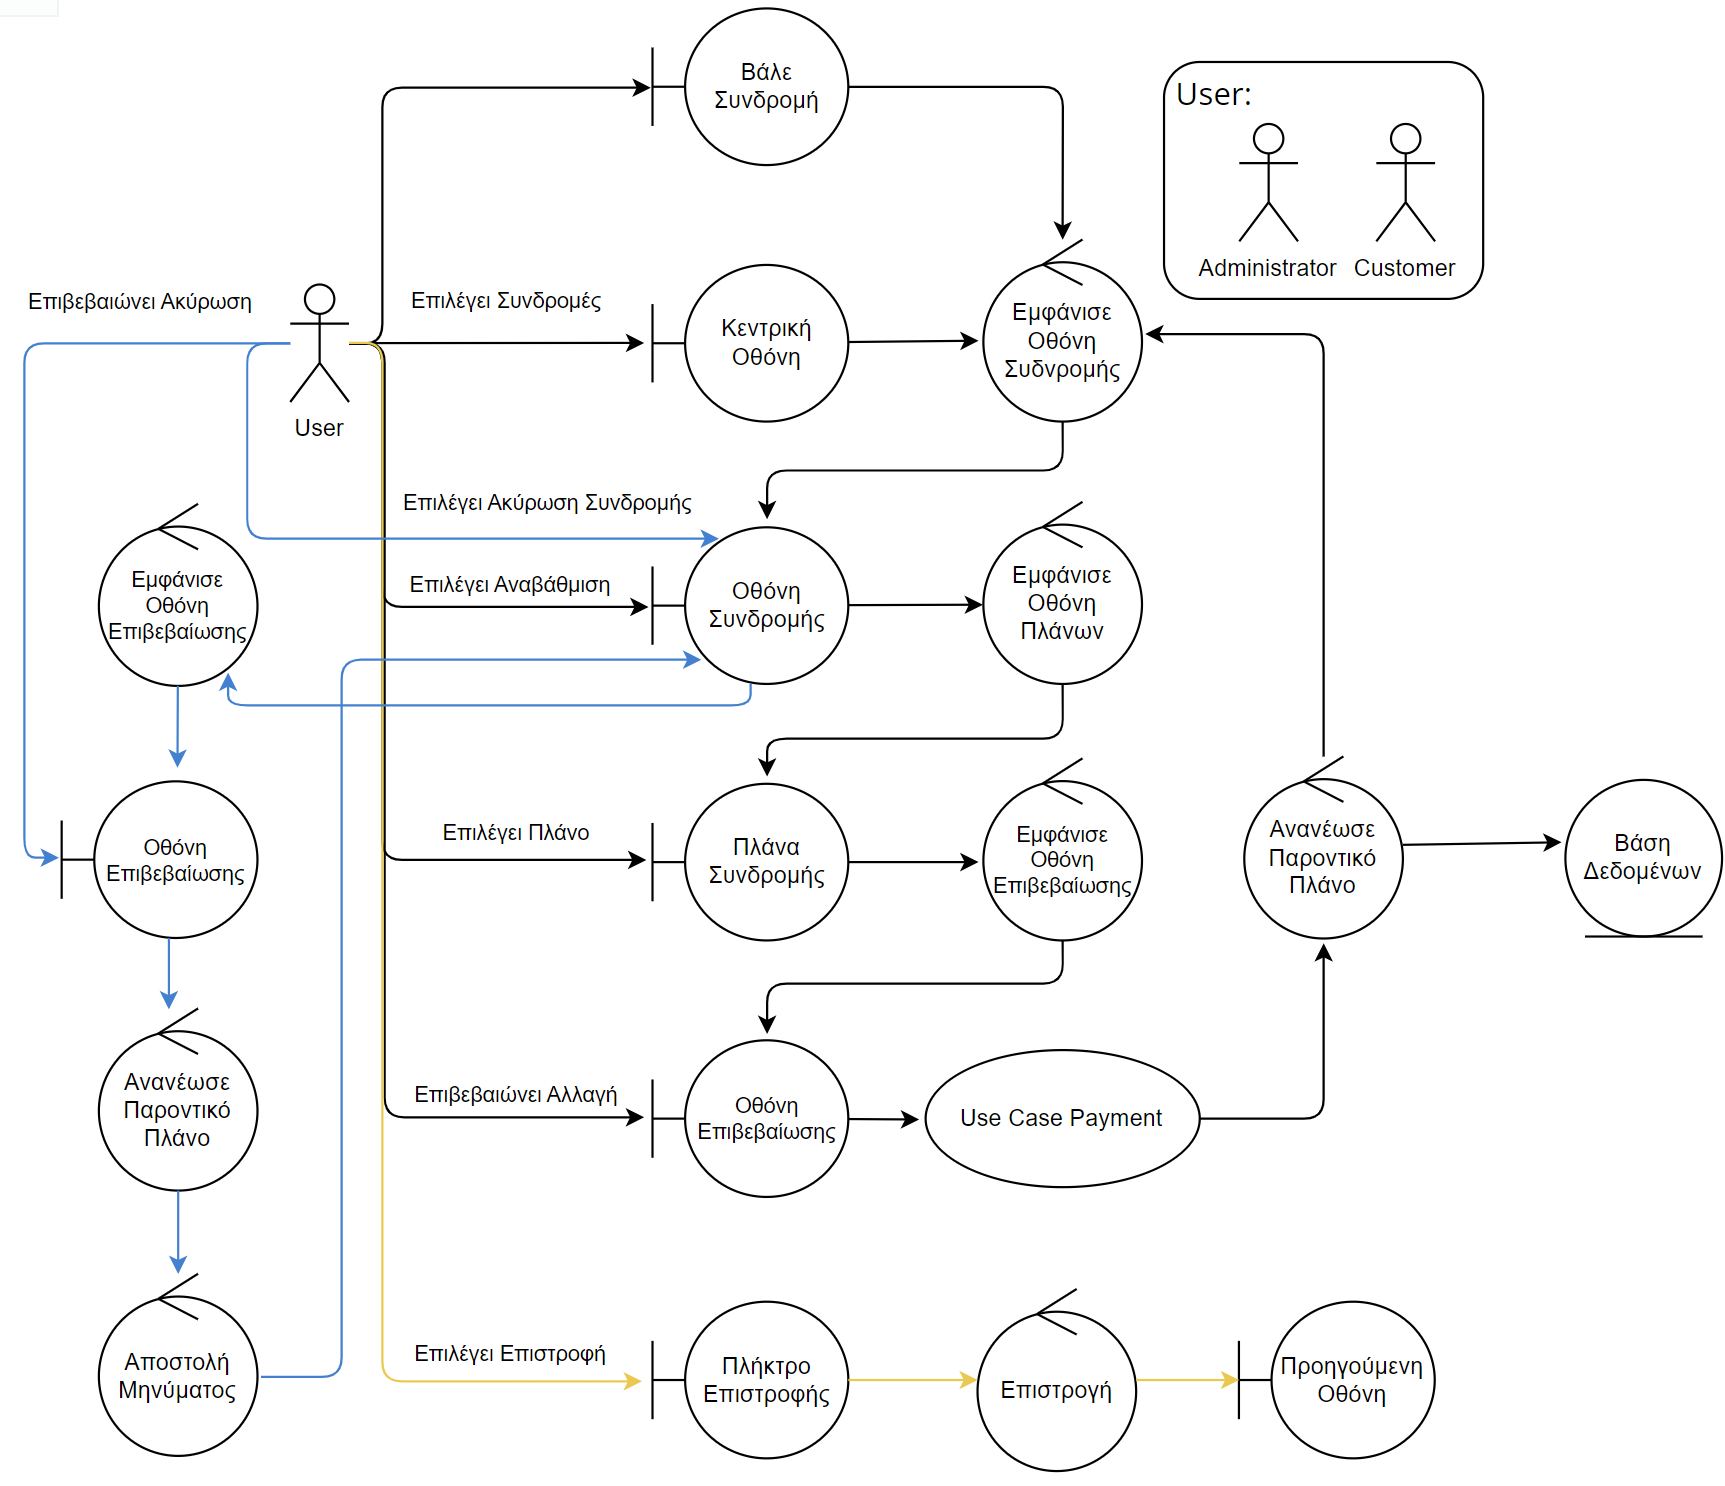
\includegraphics[width=\textwidth]{Resources/Robustness Diagram/Subscription.png}
    \caption{User είναι Διαχειριστής και Πελάτης}\label{fig:robustness-subscription}
\end{figure}

\subsection{Pet's Profile Creation}
\begin{figure}[H]
    \centering
    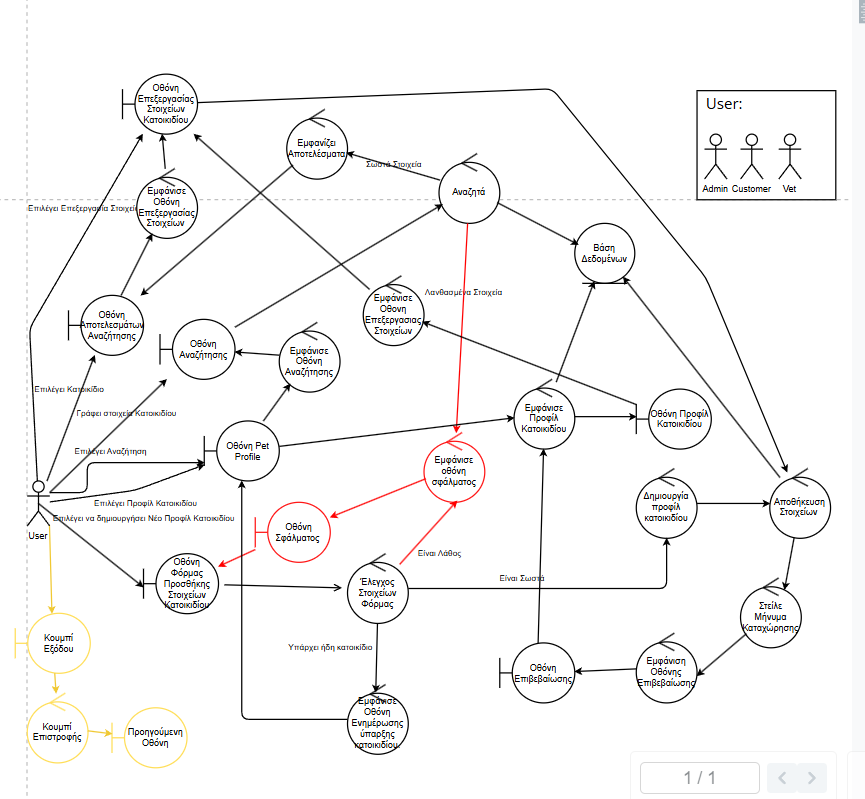
\includegraphics[width=\textwidth]{Resources/Robustness Diagram/PetProfile.png}
    \caption{User είναι Διαχειριστής, Κτηνίατρος και Πελάτης}\label{fig:robustness-pet-profile}
\end{figure}

\subsection{View Statistics}
\begin{figure}[H]
    \centering
    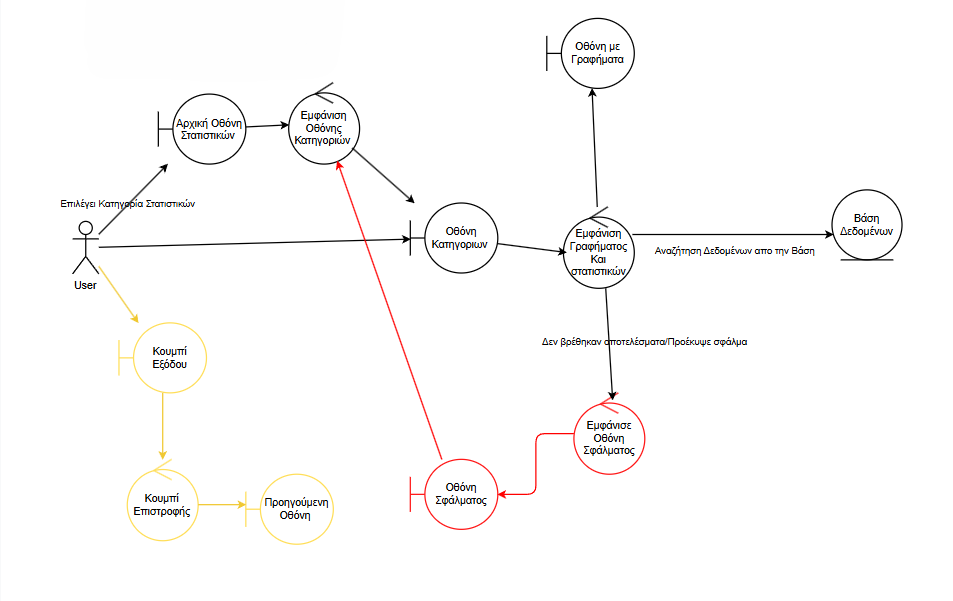
\includegraphics[width=\textwidth]{Resources/Robustness Diagram/Statistics.png}
    \caption{User είναι Διαχειριστής, Κτηνίατρος, Pet Groomer και Γραμματέας}\label{fig:robustness-view-statistics}
\end{figure}

\chapter{Use-case-v0.3}

\section{Περίληψη}

Το τρέχον κεφάλαιο περιγράφει την διαδικασία ανάπτυξης περιπτώσεων χρήσης της εφαρμογής \textit{Pet-à-Vet}. Σκοπός της αναφοράς είναι να καταγράψει τις περιπτώσεις χρήσης της εφαρμογής, καθώς και τις απαιτήσεις που προκύπτουν από αυτές. Η αναφορά αυτή είναι το αποτέλεσμα συνεργασίας πέντε μελών, οι οποίοι εργάστηκαν ομαδικά για την ανάπτυξη της εφαρμογής. Κάθε μέλος της ομάδας ανέπτυξε τουλάχιστον δύο περιπτώσεις χρήσης και σχετικές αναφορές για αυτές, οι οποίες περιγράφουν τις λειτουργίες της εφαρμογής. Κάθε περίπτωση χρήσης εξετάστηκε και ελέγχθηκε από όλα τα μέλη της ομάδας, προκειμένου να υπάρχει συνοχή και ομοιομορφία στην παρουσίαση και την περιγραφή τους. Χρησιμοποιήθκαν τα εργαλεία \textit{Word} και \textit{LaTeX} για την συγγραφή των κειμένων. % chktex 19

Στην τρίτη έκδοση, οι περιπτώσεις χρήσης και οι ροές τους έγιναν πιο απλές. % chktex 19

\section{Authentication}

\subsection{Σύντομη Περιγραφή}
Η περίπτωση χρήσης «Σύνδεση» εξυπηρετεί τον σκοπό της ταυτοποίησης του χρήστη στην εφαρμογή. Ο χρήστης εισάγει το όνομα χρήστη και τον κωδικό πρόσβασης που έχει δηλώσει κατά την εγγραφή του στην εφαρμογή. Η προκείμενη Περίπτωση Χρήσης αποτελεί βασική προϋπόθεση για τον χρήστη για να έχει την δυνατότητα να χρησιμοποιεί την εφαρμογή, αφού μόνο με προφίλ μπορεί να έχει πρόσβαση στις λειτουργίες. Για αυτόν τον λόγο, η σύνδεση ορίζεται ως το εναρκτήριο βήμα στην ροή χρήσης της εφαρμογής. Χρησιμοποιεί τις περιπτώσεις χρήσης `Sign Up' και `Sign In' % chktex 19

\subsection{Χειριστές}
\begin{itemize}
  \item Διαχειριστής
  \item Γραμματέας
  \item Κτηνίατρος
  \item Pet Groomer
  \item Πελάτης
  \item Εξωτερική βάση δεδομένων % chktex 19
\end{itemize}

\subsection{Γεγονός Έναρξης}
Η περίπτωση χρήσης ξεκινά όταν:
\begin{itemize}
  \item Ένας χρήστης μπαίνει στην εφαρμογή
\end{itemize}

\subsection{Ροή γεγονότων}

\subsubsection{Βασική Ροή}
\begin{enumerate}
  \item Ο χρήστης μπαίνει στην εφαρμογή
  \item Η περίπτωση χρήσης συνεχίζεται με την περίπτωση χρήσης `Sign In' % chktex 19
\end{enumerate}

\subsubsection{Εναλλακτικές Ροές}
\begin{enumerate}
  \item[1 ] Εγγραφή % chktex 19
        \begin{enumerate}
          \item[2.1.1 ] Η περίπτωση χρήσης συνεχίζεται με την περίπτωση χρήσης `Sign Up' % chktex 19
        \end{enumerate}
\end{enumerate}

\subsection{Ειδικές απαιτήσεις} % chktex 19
\begin{itemize}
  \item Το σύστημα πρέπει να συμμορφώνεται με τους κανόνες προστασίας προσωπικών δεδομένων (GDPR)  % chktex 19
  \item Το σύστημα πρέπει να επικοινωνεί αψεγάδιαστα με το ασφαλές περιβάλλον της τράπεζας και να μην έχει πρόσβαση σε στοιχεία κάρτας του πελάτη   % chktex 19 chktex 18
  \item Το σύστημα πρέπει να διατηρεί αρχείο καταγραφής (audit trail) όλων των τροποποιήσεων που πραγματοποιούνται. % chktex 19
\end{itemize}

\subsubsection{Μη λειτουργικές απαιτήσεις}
\begin{itemize}
  \item Το σύστημα πρέπει να παρέχει σαφή και κατανοητά μηνύματα σε περιπτώσεις εξαιρέσεων, δηλαδή, για περιπτώσεις που ο χρήστης αφήνει κενά πεδία ή εισάγει λανθασμένες τιμές σε πεδία.% chktex 19
  \item Το σύστημα πρέπει να παρέχει έναν ασφαλή τρόπο εγγραφής στον χρήστη. Το σύστημα είναι αναγκαίο να κρυπτογραφεί τα προσωπικά δεδομένα των χρηστών, να έχει δικλείδες ασφαλείας για περιπτώσεις πειρατείας ή προσπάθεια διαρροής δεδομένων, και να μην αποθηκεύει τους κωδικούς πρόσβασης σε ορατή μορφή. % chktex 19
  \item Το σύστημα πρέπει να έχει γρήγορη ανταπόκριση, και να εμφανίζει τη φόρμα εγγραφής σε χρόνο λιγότερο των 2 δευτερολέπτων, καθώς και να αποθηκεύει τα δεδομένα του χρήστη σε λιγότερο από 5 δευτερόλεπτα. % chktex 19
  \item Η διεπαφή πρέπει να είναι προσβάσιμη από κινητές συσκευές (responsive design). % chktex 19
\end{itemize}

\subsubsection{Περιβάλλον}
\begin{itemize}
  \item Web \& Mobile εφαρμογή.
\end{itemize}

\subsection{Κατάσταση εισόδου} % chktex 19
\begin{itemize}
  \item Ο χρήστης θα πρέπει να έχει επαρκή αποθηκευτικό χώρο στην συσκευή του ώστε να μπορεί να εγκαταστήσει την εφαρμογή.% chktex 19
\end{itemize}

\subsection{Κάτασταση εξόδου} % chktex 19
\begin{itemize}
  \item Αφού ολοκληρωθεί η διαδικασία της εγγραφής, το σύστημα θα περιέχει τα προσωπικά στοιχεία του χρήστη στην βάση δεδομένων.% chktex 19
  \item Ο χρήστης θα μπορεί πλέον να συνδεθεί με τα διαπιστευτήριά του και να χρησιμοποιήσει την εφαρμογή. % chktex 19
\end{itemize}
\section{Sign Up}

\subsection{Σύντομη Περιγραφή}
Η περίπτωση χρήσης «Δημιουργία Προφίλ» εξυπηρετεί τον σκοπό της δημιουργίας λογαριασμού για τον χρήστη, γεγονός που σημαίνει την εγγραφή του χρήστη στην βάση δεδομένων της εφαρμογής. Η προκείμενη Περίπτωση Χρήσης αποτελεί βασική προϋπόθεση για τον χρήστη για να έχει την δυνατότητα να χρησιμοποιεί την εφαρμογή, αφού μόνο με προφίλ μπορεί να έχει πρόσβαση στις λειτουργίες. Για αυτόν τον λόγο, η δημιουργία προφίλ ορίζεται ως το εναρκτήριο βήμα στην ροή χρήσης της εφαρμογής. % chktex 19

\subsection{Χειριστές}
\begin{itemize}
  \item Διαχειριστής
  \item Γραμματέας
  \item Κτηνίατρος
  \item Pet Groomer
  \item Πελάτης
  \item Εξωτερική βάση δεδομένων % chktex 19
\end{itemize}

\subsection{Γεγονός Έναρξης}
Η περίπτωση χρήσης ξεκινά όταν:
\begin{itemize}
  \item Ένας πελάτης, κτηνίατρος, γραμματέας ή κομμωτής διαλέξει την επιλογή «Εγγραφή», που εμφανίζεται στην αρχική οθόνη διασύνδεσης του χρήστη.  % chktex 19
\end{itemize}

\subsection{Ροή γεγονότων}

\subsubsection{Βασική Ροή}
\begin{enumerate}
  \item Ο χρήστης επιλέγει την επιλογή «Εγγραφή» στην Οθόνη Σύνδεσης/Εγγραφής.  % chktex 19
  \item Το σύστημα εμφανίζει τα πεδία που ο χρήστης θα συμπληρώσει στην Οθόνη Εγγραφής. % chktex 19
  \item Ο χρήστης συμπληρώνει τα πεδία εγγραφής με τα στοιχεία του στην Οθόνη Εγγραφής. % chktex 19
  \item Ο χρήστης επιλέγει «Έλεγχος και Επιβεβαίωση», αφού συμπληρώσει τα στοιχεία του στην Οθόνη Εγγραφής. % chktex 19
  \item Το σύστημα ελέγχει τα στοιχεία εγγραφής του χρήστη και διαπιστώνει πως είναι ορθά.  % chktex 19
  \item Το σύστημα δημιουργεί λογαριασμό για τον χρήστη και ενημερώνει την Βάση Δεδομένων με τα στοιχεία του. % chktex 19
  \item Το σύστημα ανακατευθύνει τον χρήστη στην οθόνη Σύνδεσης. % chktex 19
\end{enumerate}

\subsubsection{Εναλλακτικές Ροές}
\begin{enumerate}
  \item[1 ] Λανθασμένο πεδίο  % chktex 19
        \begin{enumerate}
          \item[5.1.1 ] Το σύστημα διαπιστώνει πως ο χρήστης έχει λάθος σε κάποιο πεδίο ή έχει αφήσει κάποιο κενό στην Οθόνη Εγγραφής. % chktex 19
          \item[5.1.2 ] Το σύστημα εμφανίζει μήνυμα «Εσφαλμένη τιμή πεδίου». % chktex 19
          \item[5.1.3 ] Ο χρήστης κλείνει το μήνυμα. % chktex 19
          \item[5.1.4 ] Το σύστημα επισημαίνει με κόκκινο το πεδίο ή τα πεδία που είναι λανθασμένα ή κενά. % chktex 19
          \item[5.1.5 ] Η Περίπτωση Χρήσης συνεχίζεται από το βήμα 3 της Βασικής Ροής.
        \end{enumerate}
  % \item[2 ] Λανθασμένο πεδίο % chktex 19
  %       \begin{enumerate}
  %         \item[6.2.1 ] Το σύστημα διαπιστώνει πως ο χρήστης έχει λάθος σε κάποιο πεδίο.% chktex 19
  %         \item[6.2.2 ] Το σύστημα εμφανίζει μήνυμα «Εσφαλμένη τιμή πεδίου».  % chktex 19
  %         \item[6.2.3 ] Ο χρήστης κλείνει το μήνυμα.% chktex 19
  %         \item[6.2.4 ] Η Περίπτωση Χρήσης συνεχίζεται από το βήμα 3 της Βασικής Ροής. % chktex 19
  %       \end{enumerate}
  \item[2 ] Επιστροφή
        \begin{enumerate}
          \item[2.2.1 ] Ο χρήστης επιλέγει την επιστροφή οποιαδήποτε στιγμή μετά το βήμα 2 % chktex 19
          \item[2.2.2 ] Το σύστημα αναγνωρίζει το αίτημα του χρήστη % chktex 19
          \item[2.2.3 ] Το σύστημα ακυρώνει την διαδικασία που ο χρήστης βρισκόταν και τον επιστρέφει στην προηγούμενη σελίδα % chktex 19
        \end{enumerate}
\end{enumerate}

\subsection{Ειδικές απαιτήσεις} % chktex 19
\begin{itemize}
  \item Το σύστημα πρέπει να συμμορφώνεται με τους κανόνες προστασίας προσωπικών δεδομένων (GDPR)  % chktex 19
  \item Το σύστημα πρέπει να επικοινωνεί αψεγάδιαστα με το ασφαλές περιβάλλον της τράπεζας και να μην έχει πρόσβαση σε στοιχεία κάρτας του πελάτη   % chktex 19 chktex 18
  \item Το σύστημα πρέπει να διατηρεί αρχείο καταγραφής (audit trail) όλων των τροποποιήσεων που πραγματοποιούνται. % chktex 19
\end{itemize}

\subsubsection{Μη λειτουργικές απαιτήσεις}
\begin{itemize}
  \item Το σύστημα πρέπει να παρέχει σαφή και κατανοητά μηνύματα σε περιπτώσεις εξαιρέσεων, δηλαδή, για περιπτώσεις που ο χρήστης αφήνει κενά πεδία ή εισάγει λανθασμένες τιμές σε πεδία.% chktex 19
  \item Το σύστημα πρέπει να παρέχει έναν ασφαλή τρόπο εγγραφής στον χρήστη. Το σύστημα είναι αναγκαίο να κρυπτογραφεί τα προσωπικά δεδομένα των χρηστών, να έχει δικλείδες ασφαλείας για περιπτώσεις πειρατείας ή προσπάθεια διαρροής δεδομένων, και να μην αποθηκεύει τους κωδικούς πρόσβασης σε ορατή μορφή. % chktex 19
  \item Το σύστημα πρέπει να έχει γρήγορη ανταπόκριση, και να εμφανίζει τη φόρμα εγγραφής σε χρόνο λιγότερο των 2 δευτερολέπτων, καθώς και να αποθηκεύει τα δεδομένα του χρήστη σε λιγότερο από 5 δευτερόλεπτα. % chktex 19
  \item Η διεπαφή πρέπει να είναι προσβάσιμη από κινητές συσκευές (responsive design). % chktex 19
\end{itemize}

\subsubsection{Περιβάλλον}
\begin{itemize}
  \item Web \& Mobile εφαρμογή.
\end{itemize}

\subsection{Κατάσταση εισόδου} % chktex 19
\begin{itemize}
  \item Ο χρήστης θα πρέπει να έχει επαρκή αποθηκευτικό χώρο στην συσκευή του ώστε να μπορεί να εγκαταστήσει την εφαρμογή.% chktex 19
\end{itemize}

\subsection{Κάτασταση εξόδου} % chktex 19
\begin{itemize}
  \item Αφού ολοκληρωθεί η διαδικασία της εγγραφής, το σύστημα θα περιέχει τα προσωπικά στοιχεία του χρήστη στην βάση δεδομένων.% chktex 19
  \item Ο χρήστης θα μπορεί πλέον να συνδεθεί με τα διαπιστευτήριά του και να χρησιμοποιήσει την εφαρμογή. % chktex 19
\end{itemize}

\section{Sign In} % chktex 19

\subsection{Σύντομη Περιγραφή}
Στην Περίπτωση Χρήσης αυτή, γίνεται η διαδικασία της ταυτοποίησης χρήστη. Συγκεκριμένα, ο χρήστης εισάγει τα διαπιστευτήρια του στο σύστημα, και αποκτά πρόσβαση στις λειτουργίες του. Όπως και η Εγγραφή, έτσι και η Σύνδεση αποτελεί αναγκαία διαδικασία, καθώς ο χρήστης μπορεί να χειριστεί την εφαρμογή μόνο μέσω λογαριασμού.% chktex 19

\subsection{Χειριστές}
\begin{itemize}
  \item Διαχειριστής
  \item Γραμματέας
  \item Κτηνίατρος
  \item Pet Groomer
  \item Πελάτης
  \item Εξωτερική βάση δεδομένων % chktex 19
\end{itemize}

\subsection{Γεγονός Έναρξης}
Η περίπτωση χρήσης ξεκινά όταν:
\begin{itemize}
  \item Ο χρήστης διαλέξει την επιλογή «Σύνδεση», που εμφανίζεται στην αρχική οθόνη διασύνδεσης του χρήστη. % chktex 19
\end{itemize}

\subsection{Ροή γεγονότων}

\subsubsection{Βασική Ροή}
\begin{enumerate}
  \item Ο χρήστης επιλέγει την επιλογή «Σύνδεση» στην Οθόνη Σύνδεσης/Εγγραφής. % chktex 19
  \item Το σύστημα εμφανίζει τα πεδία ταυτοποίησης στην Οθόνη Σύνδεσης. % chktex 19
  \item Ο χρήστης πληκτρολογεί τα στοιχεία σύνδεσής του στην Οθόνη Σύνδεσης. % chktex 19
  \item Ο χρήστης επιλέγει «Είσοδος» στην Οθόνη Σύνδεσης. % chktex 19
  \item Το σύστημα ελέγχει μέσω της αντίστοιχης λίστας με τα στοιχεία των εγγεγραμμένων χρηστών, καθώς και ελέγχει αν ο χρήστης έχει πληκτρολογήσει σωστά τα στοιχεία του και διαπιστώνει ότι ο συνδυασμός των παραπάνω δύο αντιστοιχεί σε χρήστη. % chktex 19
  \item Το σύστημα ανακατευθύνει τον χρήστη στην Αρχική Οθόνη της εφαρμογής, ανάλογα τον ρόλο του. % chktex 19
\end{enumerate}

\subsubsection{Εναλλακτικές Ροές}
\begin{enumerate}
  \item[1 ] Λανθασμένο πεδίο  % chktex 19
        \begin{enumerate}
          \item[5.1.1 ] Το σύστημα διαπιστώνει ότι ο χρήστης έχει πληκτρολογήσει κάποιο/α στοιχείο/α λάθος, ή έχει αφήσει κενά. % chktex 19
          \item[5.1.2 ] Το σύστημα εμφανίζει μήνυμα «Λάθος email ή κωδικός πρόσβασης». % chktex 19
          \item[5.1.3 ] Ο χρήστης κλείνει το μήνυμα. % chktex 19
          \item[5.1.4 ] Η Περίπτωση Χρήσης συνεχίζεται από το βήμα 3 της Βασικής Ροής. % chktex 19
        \end{enumerate}
  \item[2 ] Μη εγγεγραμμένος χρήστης % chktex 19
        \begin{enumerate}
          \item[5.2.1 ] Το σύστημα ελέγχει μέσω της αντίστοιχης λίστας με τα στοιχεία των εγγεγραμμένων χρηστών και διαπιστώνει ότι ο συνδυασμός των παραπάνω δύο στοιχείων δεν αντιστοιχεί σε χρήστη. % chktex 19
          \item[5.2.2 ] Το σύστημα εμφανίζει μήνυμα «Δεν υπάρχει χρήστης με αυτά τα στοιχεία σύνδεσης». % chktex 19
          \item[5.2.3 ] Ο χρήστης κλείνει το μήνυμα.% chktex 19
          \item[5.2.4 ] Η Περίπτωση Χρήσης μεταβαίνει στην Περίπτωση Χρήσης «Sign Up». % chktex 19
        \end{enumerate}
  \item[3 ] Επιστροφή
        \begin{enumerate}
          \item[2.3.1 ] Ο χρήστης επιλέγει την επιστροφή οποιαδήποτε στιγμή μετά το βήμα 2 % chktex 19
          \item[2.3.2 ] Το σύστημα αναγνωρίζει το αίτημα του χρήστη % chktex 19
          \item[2.3.3 ] Το σύστημα ακυρώνει την διαδικασία που ο χρήστης βρισκόταν και τον επιστρέφει στην προηγούμενη σελίδα % chktex 19
        \end{enumerate}
\end{enumerate}

\subsection{Ειδικές απαιτήσεις} % chktex 19
\begin{itemize}
  \item Το σύστημα πρέπει να συμμορφώνεται με τους κανόνες προστασίας προσωπικών δεδομένων (GDPR)  % chktex 19
  \item Το σύστημα πρέπει να επικοινωνεί αψεγάδιαστα με το ασφαλές περιβάλλον της τράπεζας και να μην έχει πρόσβαση σε στοιχεία κάρτας του πελάτη   % chktex 19 chktex 18
  \item Το σύστημα πρέπει να διατηρεί αρχείο καταγραφής (audit trail) όλων των τροποποιήσεων που πραγματοποιούνται. % chktex 19
\end{itemize}

\subsubsection{Μη λειτουργικές απαιτήσεις}
\begin{itemize}
  \item Το σύστημα πρέπει να παρέχει σαφή και κατανοητά μηνύματα σε περιπτώσεις εξαιρέσεων, δηλαδή, για περιπτώσεις που ο χρήστης αφήνει κενά πεδία ή εισάγει λανθασμένες τιμές σε πεδία.% chktex 19
  \item Το σύστημα πρέπει να παρέχει έναν ασφαλή τρόπο εγγραφής στον χρήστη. Το σύστημα είναι αναγκαίο να κρυπτογραφεί τα προσωπικά δεδομένα των χρηστών, να έχει δικλείδες ασφαλείας για περιπτώσεις πειρατείας ή προσπάθεια διαρροής δεδομένων, και να μην αποθηκεύει τους κωδικούς πρόσβασης σε ορατή μορφή. % chktex 19
  \item Το σύστημα πρέπει να έχει γρήγορη ανταπόκριση, και να εμφανίζει τη φόρμα εγγραφής σε χρόνο λιγότερο των 2 δευτερολέπτων, καθώς και να αποθηκεύει τα δεδομένα του χρήστη σε λιγότερο από 5 δευτερόλεπτα. % chktex 19
  \item Η διεπαφή πρέπει να είναι προσβάσιμη από κινητές συσκευές (responsive design). % chktex 19
\end{itemize}

\subsubsection{Περιβάλλον}
\begin{itemize}
  \item Web \& Mobile εφαρμογή.
\end{itemize}

\subsection{Κατάσταση εισόδου} % chktex 19
\begin{itemize}
  \item Ο χρήστης πρέπει να έχει δημιουργήσει λογαριασμό/προφίλ για να μπορέσει να συνδεθεί στην εφαρμογή. % chktex 19
  \item Η βάση δεδομένων να είναι προσβάσιμη και λειτουργική κατά την διαδικασία της σύνδεσης. % chktex 19
\end{itemize}

\subsection{Κάτασταση εξόδου} % chktex 19
\begin{itemize}
  \item Ο χρήστης είναι συνδεδεμένος με επιτυχία στην εφαρμογή και έχει πρόσβαση σε όλες τις λειτουργίες του, ανάλογα με τον ρόλο του. % chktex 19
\end{itemize}

\section{Customer Management}

\subsection{Σύντομη Περιγραφή}
Η περίπτωση χρήσης "Customer Management" επιτρέπει στους διαχειριστές της κτηνιατρικής κλινικής και στο προσωπικό υποδοχής να διαχειρίζονται πλήρως τα προφίλ των πελατών (ιδιοκτητών κατοικίδιων). Αυτό περιλαμβάνει την καταχώρηση νέων πελατών, την ενημέρωση των στοιχείων τους, την προβολή του ιστορικού επισκέψεων, την αντιστοίχιση με τα κατοικίδιά τους, και την παρακολούθηση οικονομικών συναλλαγών. Η περίπτωση χρήσης περιλαμβάνει επίσης τις λειτουργίες "Sort" και "Filter" για την αποτελεσματικότερη διαχείριση του καταλόγου πελατών. % chktex 18 % chktex 19

\subsection{Χειριστές}
\begin{itemize}
  \item Διαχειριστής συστήματος
  \item Γραμματέας
  \item Εξωτερική βάση δεδομένων % chktex 19
\end{itemize}

\subsection{Γεγονός Έναρξης}
Η περίπτωση χρήσης ξεκινά όταν:
\begin{itemize}
  \item Ένας διαχειριστής, κτηνίατρος ή υπάλληλος υποδοχής επιλέγει την επιλογή "Customer Management" από το κεντρικό μενού % chktex 18 % chktex 19
        %   \item Ένας νέος πελάτης εγγράφεται στο σύστημα μέσω της διαδικτυακής πλατφόρμας
        %   \item Το προσωπικό χρειάζεται να αναζητήσει πληροφορίες για έναν πελάτη
        %   \item Ο ιδιοκτήτης κατοικίδιου συνδέεται στο λογαριασμό του για να επεξεργαστεί τα στοιχεία του
\end{itemize}

\subsection{Ροή γεγονότων}

\subsubsection{Βασική Ροή}
\begin{enumerate}
  \item Ο χρήστης μπαίνει στην ενότητα "Customer Management". % chktex 18
  \item Το σύστημα εμφανίζει στην Οθόνη "Customer Management" μια λίστα με τους υπάρχοντες πελάτες από την βάση δεδομένων. % chktex 19 chktex 18
  \item Ο χρήστης επιλέγει τη προσθήκη πελάτη στην Οθόνη "Customer Management". % chktex 19 chktex 18
  \item Το σύστημα εμφανίζει φόρμα με τα πεδία στην Οθόνη Φόρμας Προσθήκης Πελάτη. %(ονοματεπώνυμο, στοιχεία επικοινωνίας, διεύθυνση κτλ.). % chktex 19
  \item Ο χρήστης συμπληρώνει τα στοιχεία και υποβάλλει τη φόρμα στην Οθόνη Φόρμας Προσθήκης Πελάτη.
  \item Το σύστημα ελέγχει τα δεδομένα, δημιουργεί και αποθηκεύει το νέο προφίλ πελάτη στη βάση δεδομένων. % chktex 19
  \item Το σύστημα αποστέλλει αυτόματα email/SMS καλωσορίσματος με οδηγίες ενεργοποίησης λογαριασμού στο νέο πελάτη. % chktex 19
  \item Το σύστημα εμφανίζει Οθόνη Επιβεβαίωσης της δημιουργίας του προφίλ και εμφανίζει τη νέα λίστα με τους πελάτες στη σελίδα "Customer Management". % chktex 19 chktex 18
\end{enumerate}

\subsubsection{Εναλλακτικές Ροές}
\begin{enumerate}
  \item[1 ] "Search"(/προβολή) υπάρχοντος πελάτη: % chktex 18 chktex 36
        \begin{enumerate}
          \item[3.1.1 ] Ο χρήστης επιλέγει την επιλογή αναζήτησης στην Οθόνη "Customer Management" %chktex 19 chktex 18
          \item[3.1.2 ] Ο χρήστης εισάγει κριτήρια αναζήτησης στην Οθόνη Αναζήτησης %(όνομα, email, τηλέφωνο, κ.λπ.)
          \item[3.1.3 ] Το σύστημα αναζητά το πελάτη στη βάση δεδομένων και εμφανίζει τα αποτελέσματα που ταιριάζουν στην Οθόνη Αποτελέσματα Αναζήτησης % chktex 19
          \item[3.1.4 ] Ο χρήστης επιλέγει τον επιθυμητό πελάτη από τα αποτελέσματα και προβάλει τα στοχεία του
          \item[3.1.5 ] Ο χρήστης κλείνει το παράθυρο αναζήτησης και επιστρέφει στο βήμα 2 της βασικής ροής
        \end{enumerate}
  \item[2 ] Επεξεργασία προφίλ πελάτη:
        \begin{enumerate}
          \item[3.2.1 ] Ο χρήστης επιλέγει την επιλογή αναζήτησης στην Οθόνη "Customer Management" %chktex 19 chktex 18
          \item[3.2.2 ] Ο χρήστης εισάγει κριτήρια αναζήτησης στην Οθόνη Αναζήτησης %(όνομα, email, τηλέφωνο, κ.λπ.)
          \item[3.2.3 ] Το σύστημα αναζητά το πελάτη στη βάση δεδομένων και εμφανίζει τα αποτελέσματα που ταιριάζουν στην Οθόνη Αποτελέσματα Αναζήτησης % chktex 19
          \item[3.2.4 ] Ο χρήστης επιλέγει τον επιθυμητό πελάτη από τα αποτελέσματα και επεξεργάζεται τα στοιχεία του στην Οθόνη Επεξεργασίας Στοιχείων Πελάτη % chktex 19
          \item[3.2.5 ] Ο χρήστης αποθηκεύει τις αλλαγές στη Βάση Δεδομένων και επιστρέφει στο βήμα 2 της βασικής ροής. % chktex 19
        \end{enumerate}
  \item[3 ] Χρήση περίπτωσης Filter:
        \begin{enumerate}
          \item[3.3.1 ] Ο χρήστης επιλέγει το "Filter"  % chktex 18
          \item[3.3.2 ] Το σύστημα εκτελεί την περίπτωση χρήσης "Filter" για πελάτες % chktex 18
          \item[3.3.3 ] Μετά την ολοκλήρωση του φιλτραρίσματος, το σύστημα επιστρέφει στη λίστα πελατών
        \end{enumerate}
  \item[4 ] Λανθασμένη εισαγωγή δεδομένων: % chktex 19
        \begin{enumerate}
          \item[3.4.1 ] Ο χρήστης επιλέγει τη προσθήκη πελάτη στην Οθόνη Φόρμας Προσθήκης Πελάτη
          \item[3.4.2 ] Ο χρήστης εισάγει τα στοιχεία του νέου πελάτη σε λανθασμένη μορφή στην Οθόνη Φόρμας Προσθήκης Πελάτη
          \item[3.4.3 ] Το σύστημα εμφανίζει Οθόνη Σφάλαματος και οδηγεί τον χρήστη στο βήμα 4 της βασικής ροής % chktex 19
        \end{enumerate}
  \item[5 ] Επιστροφή
        \begin{enumerate}
          \item[2.5.1 ] Ο χρήστης επιλέγει την επιστροφή οποιαδήποτε στιγμή μετά το βήμα 2 % chktex 19
          \item[2.5.2 ] Το σύστημα ακυρώνει την διαδικασία που ο χρήστης βρισκόταν και τον επιστρέφει στην Οθόνη "Customer Management" %chktex 19 chktex 18
        \end{enumerate}
  % \item[7 ] Ακύρωση επεξεργασίας:
  %       \begin{enumerate}
  %         \item[3.7.1 ] Ο χρήστης επιλέγει την επιλογή αναζήτησης
  %         \item[3.7.2 ] Ο χρήστης εισάγει κριτήρια αναζήτησης %(όνομα, email, τηλέφωνο, κ.λπ.)
  %         \item[3.7.3 ] Το σύστημα εμφανίζει τα αποτελέσματα που ταιριάζουν
  %         \item[3.7.4 ] Ο χρήστης επιλέγει την επεξεργασία του επιθυμητού πελάτη από τα αποτελέσματα
  %         \item[3.7.5 ] Ο χρήστης επιλέγει την επιλογή ακύρωσης
  %         \item[3.7.6 ] Το σύστημα εμφανίζει μήνυμα επιβεβαίωσης και οδηγεί τον χρήστη στο βήμα 2 της βασικής ροής % chktex 19
  %       \end{enumerate}
  % \item[6 ] Λανθασμένα κριτήρια αναζήτησης:
  %       \begin{enumerate}
  %         \item[3.6.1 ] Ο χρήστης επιλέγει την επιλογή αναζήτησης στην Οθόνη "Customer Management". % chktex 19 chktex 18
  %         \item[3.6.2 ] Ο χρήστης εισάγει λανθασμένα κριτήρια αναζήτησης στην Οθόνη Αναζήτησης
  %         \item[3.6.3 ] Το σύστημα εμφανίζει μήνυμα λάθους και οδηγεί τον χρήστη στο βήμα 2 της εναλλακτικής ροής % chktex 19
  %       \end{enumerate}
  % \item[8 ] Πάτημα πελάτη:
  %       \begin{enumerate}
  %         \item[3.8.1 ] Ο χρήστης επιλέγει έναν πελάτη από αυτούς που εμφανίζονται αρχικά στην οθόνη
  %         \item[3.8.2 ] Το σύστημα εμφανίζει τα στοιχεία του επιλεγμένου πελάτη
  %         \item[3.8.3 ] Ο χρήστης πατάει κλείσιμο και το σύστημα τον γυρνάει στο βήμα 2 της βασικής ροής
  %       \end{enumerate}
\end{enumerate}

\subsection{Ειδικές απαιτήσεις} % chktex 19
\begin{itemize}
  \item Το σύστημα πρέπει να συμμορφώνεται με τους κανονισμούς GDPR για την προστασία προσωπικών δεδομένων % chktex 19
  \item Τα δεδομένα των πελατών θα πρέπει να κρυπτογραφούνται κατά την αποθήκευση % chktex 19
  \item Η πρόσβαση στα οικονομικά στοιχεία περιορίζεται σε χρήστες με ειδική εξουσιοδότηση % chktex 19
  \item Το σύστημα πρέπει να διατηρεί αρχείο καταγραφής όλων των τροποποιήσεων (audit trail) % chktex 19
  \item Υποστήριξη μαζικής εισαγωγής πελατών μέσω αρχείου CSV
\end{itemize}

\subsubsection{Μη λειτουργικές απαιτήσεις}
\begin{itemize}
  \item Ο χρόνος απόκρισης για αναζήτηση πελατών πρέπει να είναι λιγότερος από 2 δευτερόλεπτα ακόμα και με βάση δεδομένων 10.000+ πελατών % chktex 19
  \item Το σύστημα πρέπει να παραμένει λειτουργικό ακόμα και με περιορισμένη συνδεσιμότητα στο διαδίκτυο, διατηρώντας τοπικό αντίγραφο των πιο πρόσφατων συναλλαγών % chktex 19
  \item Το περιβάλλον χρήσης πρέπει να είναι προσβάσιμο από άτομα με αναπηρίες (WCAG 2.1 επίπεδο AA) % chktex 19
  \item Το σύστημα πρέπει να υποστηρίζει πολλαπλές γλώσσες (Ελληνικά και Αγγλικά αρχικά)
\end{itemize}

\subsubsection{Περιβάλλον}
\begin{itemize}
  \item Διαδικτυακή πλατφόρμα προσβάσιμη μέσω φυλλομετρητών (Chrome, Firefox, Safari, Edge) % chktex 19
  \item Εφαρμογή για κινητές συσκευές (iOS και Android)
\end{itemize}

\subsection{Κατάσταση εισόδου} % chktex 19
\begin{itemize}
  \item Ο χρήστης έχει συνδεθεί στο σύστημα με τα κατάλληλα διαπιστευτήρια % chktex 19
  \item Η βάση δεδομένων του συστήματος είναι προσβάσιμη και λειτουργική % chktex 19
\end{itemize}

\subsection{Κάτασταση εξόδου} % chktex 19
\begin{itemize}
  \item Τα στοιχεία του πελάτη έχουν καταχωρηθεί ή ενημερωθεί επιτυχώς στη βάση δεδομένων % chktex 19
  \item Όλες οι ενέργειες έχουν καταγραφεί στο αρχείο ιστορικού του συστήματος
  \item Έχουν σταλεί οι κατάλληλες ειδοποιήσεις στους εμπλεκόμενους (π.χ. email επιβεβαίωσης στον πελάτη)  % chktex 12 % chktex 19
  \item Ο χρήστης επιστρέφει στην κεντρική οθόνη διαχείρισης πελατών % ή προχωρά σε σχετική λειτουργία (π.χ. προγραμματισμός ραντεβού) % chktex 19
\end{itemize}

\subsection{Σημεία Επέκτασης}
\begin{itemize}
  \item Ο χρήστης μπορεί να φιλτράρει τα αποτελέσματα που εμφανίζονται στην οθόνη (`Filter') % chktex 19
\end{itemize}

\section{Filter}

\subsection{Σύντομη Περιγραφή}
Η περίπτωση χρήσης "Filter" επιτρέπει στους χρήστες να φιλτράρουν τη λίστα βάσει συγκεκριμένων κριτηρίων, περιορίζοντας τα αποτελέσματα μόνο στα στοιχεία που πληρούν τις καθορισμένες συνθήκες. % chktex 18 % chktex 19

\subsection{Χειριστές}
\begin{itemize}
  \item Διαχειριστής συστήματος
  \item Γραμματέας
  \item Κτηνίατρος
  \item Πελάτης
  \item Εξωτερική βάση δεδομένων % chktex 19
\end{itemize}

\subsection{Γεγονός Έναρξης}
Η περίπτωση χρήσης ξεκινά όταν:
\begin{itemize}
  \item Ο χρήστης επιλέγει την επιλογή φιλτραρίσματος από τη λίστα % chktex 18 % chktex 19
\end{itemize}

\subsection{Ροή γεγονότων}

\subsubsection{Βασική Ροή}
\begin{enumerate}
  \item Ο χρήστης επιλέγει την επιλογή φιλτραρίσματος στην Οθόνη με Δεδομένα % chktex 19
  \item Το σύστημα εμφανίζει τα διαθέσιμα κριτήρια φιλτραρίσματος και ταξινόμησης στην Οθόνη Φιλτραρίσματος % (κατάσταση λογαριασμού, ημερομηνία εγγραφής, κατοικίδιο, κ.λπ.) % chktex 19
  \item Ο χρήστης επιλέγει το επιθυμητό κριτήριο/α φιλτραρίσματος στην Οθόνη Φιλτραρίσματος
  \item Ο χρήστης εισάγει τις τιμές του κριτηρίου φιλτραρίσματος στην Οθόνη Φιλτραρίσματος
  \item Ο χρήστης επιλέγει το επιθυμητό κριτήριο ταξινόμησης στην Οθόνη Φιλτραρίσματος
  \item Το σύστημα εφαρμόζει το φίλτρο και την ταξινόμηση στη λίστα με τα δεδομένα από την Βάση Δεδομένων % chktex 19
  \item Το σύστημα εμφανίζει τη φιλτραρισμένη λίστα δεδομένων στην Οθόνη με Δεδομένα % chktex 19
\end{enumerate}

\subsubsection{Εναλλακτικές Ροές}
\begin{enumerate}
  % \item[1 ] Προσθήκη επιπλέον φίλτρου:
  %       \begin{enumerate}
  %         \item[6.1.1 ] Μετά το βήμα 6, ο χρήστης επιλέγει προσθήκη επιπλέον κριτηρίου φιλτραρίσματος
  %         \item[6.1.2 ] Το σύστημα εμφανίζει τα διαθέσιμα κριτήρια φιλτραρίσματος % chktex 19
  %         \item[6.1.3 ] Ο χρήστης επιλέγει το επιπλέον κριτήριο και εισάγει τις τιμές
  %         \item[6.1.4 ] Το σύστημα εφαρμόζει τον συνδυασμό φίλτρων στη λίστα % chktex 19
  %         \item[6.1.5 ] Το σύστημα εμφανίζει την ενημερωμένη φιλτραρισμένη λίστα
  %       \end{enumerate}
  \item[1 ] Απαλοιφή φίλτρων:
        \begin{enumerate}
          \item[3.1.1 ] Ο χρήστης επιλέγει να καθαρίσει όλα τα φίλτρα στην Οθόνη Φιλτραρίσματος
          \item[3.1.2 ] Το σύστημα αφαιρεί όλα τα εφαρμοσμένα φίλτρα από τη λίστα με τα δεδομένα % chktex 19
          \item[3.1.3 ] Το σύστημα εμφανίζει την πλήρη λίστα χωρίς φιλτράρισμα στην Οθόνη με Δεδομένα % chktex 19
        \end{enumerate}
  \item[2 ] Κανένα αποτέλεσμα:
        \begin{enumerate}
          \item[7.2.1 ] Το σύστημα δεν βρίσκει στοχεία στη Βάση Δεδομένων που να ικανοποιούν τα κριτήρια % chktex 19
          \item[7.2.2 ] Το σύστημα εμφανίζει μήνυμα ότι δεν βρέθηκαν αποτελέσματα με αυτά τα κριτήρια στη Οθόνη Σφάλματος % chktex 19
        \end{enumerate}
  \item[3 ] Επιστροφή
        \begin{enumerate}
          \item[3.3.1 ] Ο χρήστης επιλέγει την επιστροφή οποιαδήποτε στιγμή μετά το βήμα 4 στην Οθόνη Φιλτραρίσματος ή Σφάλματος % chktex 19
          \item[3.3.2 ] Το σύστημα ακυρώνει την διαδικασία που ο χρήστης βρισκόταν και τον επιστρέφει στην Οθόνη με Δεδομένα % chktex 19
        \end{enumerate}
\end{enumerate}

\subsection{Ειδικές απαιτήσεις} % chktex 19
\begin{itemize}
  \item Υποστήριξη σύνθετων κριτηρίων φιλτραρίσματος με λογικούς τελεστές (AND, OR)
  \item Δυνατότητα αποθήκευσης συχνά χρησιμοποιούμενων φίλτρων
  \item Οπτική ένδειξη των ενεργών φίλτρων στην οθόνη % chktex 19
\end{itemize}

\subsection{Κατάσταση εισόδου} % chktex 19
\begin{itemize}
  \item Ο χρήστης βρίσκεται στην οθόνη προβολής λίστας
  \item Υπάρχουν στοιχεία καταχωρημένοι στο σύστημα
\end{itemize}

\subsection{Κάτασταση εξόδου} % chktex 19
\begin{itemize}
  \item Η λίστα εμφανίζεται φιλτραρισμένη σύμφωνα με τα επιλεγμένα κριτήρια
\end{itemize}

\section{Warehouse Management}

\subsection{Σύντομη Περιγραφή}
Η περίπτωση χρήσης "Warehouse Management" αποτελεί την κεντρική λειτουργία διαχείρισης αποθήκης της κτηνιατρικής κλινικής. Περιλαμβάνει έξι βασικές υπο-περιπτώσεις χρήσης: % chktex 18 % chktex 19
\begin{itemize}
  \item Perform Inventory --- Εκτέλεση απογραφών αποθέματος
  \item Manage Orders --- Διαχείριση παραγγελιών προς προμηθευτές
        % \item Search Products --- Αναζήτηση και εύρεση προϊόντων
        % \item Generate Reports --- Δημιουργία αναφορών αποθήκης
        % \item Monitor Expiration --- Παρακολούθηση ημερομηνιών λήξης
\end{itemize}
Η περίπτωση χρήσης "Manage Products" επιτρέπει στους εξουσιοδοτημένους χρήστες να διαχειρίζονται τα προϊόντα της κτηνιατρικής κλινικής. Αυτό περιλαμβάνει την προσθήκη νέων προϊόντων, την επεξεργασία υπαρχόντων, την ενημέρωση των τιμών και των χαρακτηριστικών τους, καθώς και την κατηγοριοποίησή τους. Μέσω αυτών των λειτουργιών, το σύστημα επιτρέπει την ολοκληρωμένη διαχείριση του αποθέματος, συμπεριλαμβανομένων φαρμάκων, αναλωσίμων, τροφών και προϊόντων περιποίησης. % chktex 19 chktex 18

\subsection{Χειριστές}
\begin{itemize}
  \item Διαχειριστής συστήματος
  \item Κτηνίατρος
  \item Γραμματέας
  \item Εξωτερική βάση δεδομένων % chktex 19
\end{itemize}

\subsection{Γεγονός Έναρξης}
Η περίπτωση χρήσης ξεκινά όταν:
\begin{itemize}
  \item Ένας εξουσιοδοτημένος χρήστης επιλέγει την ενότητα "Warehouse Management" % chktex 18 % chktex 19
\end{itemize}

\subsection{Ροή γεγονότων}

\subsubsection{Βασική Ροή}
\begin{enumerate}
  \item Ο χρήστης εισέρχεται στο σύστημα διαχείρισης αποθήκης. % chktex 19
  \item Το σύστημα εμφανίζει στην Οθόνη `Warehouse Management' τις διαθέσιμες επιλογές (π.χ. "Manage Products", "Manage Orders", "Perform Inventory"). % chktex 19 chktex 18
  \item Ο χρήστης επιλέγει την ενότητα "Manage Products" στην Οθόνη `Warehouse Management'. % chktex 18 % chktex 19
  \item Το σύστημα εμφανίζει μια λίστα με τα υπάρχοντα προϊόντα από την Βάση Δεδομένων στην Οθόνη `Manage Products'. % chktex 19
  \item Ο χρήστης επιλέγει την προσθήκη νέου προϊόντος στην Οθόνη `Manage Products'. % chktex 19.
  \item Το σύστημα εμφανίζει φόρμα με τα απαραίτητα πεδία στην Οθόνη Φόρμας Προσθήκης Προϊόντος. %(κωδικός, όνομα, κατηγορία, προμηθευτής, τιμή αγοράς, τιμή πώλησης, ελάχιστο απόθεμα, μονάδα μέτρησης, κτλ.). % chktex 19
  \item Ο χρήστης συμπληρώνει τα στοιχεία και υποβάλλει τη φόρμα στην Οθόνη Φόρμας Προσθήκης Προϊόντος.
  \item Το σύστημα ελέγχει και επικυρώνει τα δεδομένα και αποθηκεύει το νέο προϊόν στη Βάση Δεδομένων. % chktex 19
  \item Το σύστημα δημιουργεί το προϊόν και επιβεβαιώνει τον χρήστη για την επιτυχή προσθήκη του προϊόντος στην Οθόνη Ενημέρωσης Χρήστη. % chktex 19
  \item Το σύστημα επιστρέφει στην Οθόνη `Manage Products' με το νέο προϊόν προστιθέμενο.
\end{enumerate}

\subsubsection{Εναλλακτικές Ροές}
\begin{enumerate}
  \item[1 ] Επεξεργασία υπάρχοντος προϊόντος:
        \begin{enumerate}
          \item[5.1.1 ] Ο χρήστης επιλέγει ένα προϊόν από τη λίστα στην Οθόνη `Manage Products'.
          \item[5.1.2 ] Το σύστημα εμφανίζει τη φόρμα με τα τρέχοντα στοιχεία του προϊόντος στην Οθόνη Φόρμας Επεξεργασίας Προϊόντος.
          \item[5.1.3 ] Ο χρήστης τροποποιεί τα επιθυμητά πεδία και υποβάλλει τη φόρμα στην Οθόνη Φόρμας Επεξεργασίας Προϊόντος. % chktex 19
          \item[5.1.4 ] Το σύστημα ελέγχει, επικυρώνει και αποθηκεύει τις αλλαγές στη Βάση Δεδομένων. % chktex 19
          \item[5.1.5 ] Το σύστημα επιστρέφει στην Οθόνη `Manage Products' με το προϊόν ενημερωμένο.
        \end{enumerate}
  \item[2 ] Διαγραφή προϊόντος:
        \begin{enumerate}
          \item[5.2.1 ] Ο χρήστης επιλέγει ένα προϊόν από τη λίστα στην Οθόνη `Manage Products'
          \item[5.2.2 ] Ο χρήστης επιλέγει να διαγράψει το προϊόν στην Οθόνη `Manage Products' % chktex 19
          \item[5.2.3 ] Το σύστημα ζητά επιβεβαίωση για τη διαγραφή του προϊόντος στην Οθόνη Ενημέρωσης Χρήστη% chktex 19
          \item[5.2.4 ] Ο χρήστης επιβεβαιώνει την διαγραφή του προϊόντος στην Οθόνη Ενημέρωσης % chktex 19
          \item[5.2.5 ] Το σύστημα διαγράφει το προϊόν από τη Βάση Δεδομένων % chktex 19
          \item[5.2.6 ] Το σύστημα ενημερώνει τη λίστα προϊόντων και επιστρέφει στην Οθόνη `Manage Products' % chktex 19
        \end{enumerate}
        % \item[3 ] Φιλτράρισμα προϊόντων:
        %       \begin{enumerate}
        %         \item[3.3.1 ] Ο χρήστης επιλέγει κριτήρια φιλτραρίσματος %(κατηγορία, προμηθευτής, κατάσταση)
        %         \item[3.3.2 ] Το σύστημα εφαρμόζει τα φίλτρα στη λίστα προϊόντων
        %         \item[3.3.3 ] Το σύστημα εμφανίζει τα φιλτραρισμένα αποτελέσματα
        %       \end{enumerate}
  \item[3 ] Αναζήτηση προϊόντων:
        \begin{enumerate}
          \item[5.3.1 ] Ο χρήστης αναζητά το προϊόν που θέλει στην Οθόνη `Manage Products' % chktex 19
          \item[5.3.2 ] Το σύστημα αναζητά προϊόντα που ταιριάζουν στη Βάση Δεδομένων % chktex 19
          \item[5.3.3 ] Το σύστημα εμφανίζει τα αποτελέσματα της αναζήτησης στη Οθόνη `Manage Products' % chktex 19
        \end{enumerate}
        % \item[5 ] Μαζική εισαγωγή προϊόντων:
        %       \begin{enumerate}
        %         \item[5.1 ] Ο χρήστης επιλέγει την επιλογή μαζικής εισαγωγής
        %         \item[5.2 ] Το σύστημα εμφανίζει οδηγίες για το απαιτούμενο format του αρχείου
        %         \item[5.3 ] Ο χρήστης μεταφορτώνει αρχείο CSV/Excel με τα προϊόντα
        %         \item[5.4 ] Το σύστημα επικυρώνει το αρχείο και εμφανίζει προεπισκόπηση των δεδομένων
        %         \item[5.5 ] Ο χρήστης επιβεβαιώνει την εισαγωγή
        %         \item[5.6 ] Το σύστημα εισάγει τα προϊόντα και εμφανίζει αναφορά με τα αποτελέσματα
        %       \end{enumerate}
        % \item[6 ] Διπλότυπος κωδικός προϊόντος:
        %       \begin{enumerate}
        %         \item[6.1 ] Ο χρήστης εισάγει κωδικό προϊόντος που ήδη υπάρχει
        %         \item[6.2 ] Το σύστημα ανιχνεύει τον διπλότυπο κωδικό
        %         \item[6.3 ] Το σύστημα εμφανίζει μήνυμα σφάλματος
        %         \item[6.4 ] Ο χρήστης διορθώνει τον κωδικό και συνεχίζει
        %       \end{enumerate}
        % \item[7 ] Εξαγωγή καταλόγου προϊόντων:
        %       \begin{enumerate}
        %         \item[7.1 ] Ο χρήστης επιλέγει την επιλογή εξαγωγής
        %         \item[7.2 ] Το σύστημα προσφέρει επιλογές μορφής εξαγωγής (CSV, Excel, PDF)
        %         \item[7.3 ] Ο χρήστης επιλέγει την επιθυμητή μορφή
        %         \item[7.4 ] Το σύστημα δημιουργεί και παρέχει το αρχείο για λήψη
        %       \end{enumerate}
  \item[4 ] Επιστροφή
        \begin{enumerate}
          \item[5.4.1 ] Ο χρήστης επιλέγει την επιστροφή οποιαδήποτε στιγμή μετά το βήμα 5 % chktex 19
          \item[5.4.2 ] Το σύστημα ακυρώνει την διαδικασία που ο χρήστης βρισκόταν και τον επιστρέφει στην προηγούμενη οθόνη % chktex 19
        \end{enumerate}
  \item[5 ] Perform Inventory
        \begin{enumerate}
          \item[3.5.1 ] Ο χρήστης επιλέγει την ενότητα `Perform Inventory'
          \item[3.5.2 ] Το σύστημα συνεχίζει με την περίπτωση χρήσης `Perform Inventory'
        \end{enumerate}
  \item[6 ] Manage Orders
        \begin{enumerate}
          \item[3.6.1 ] Ο χρήστης επιλέγει την ενότητα `Manage Orders'
          \item[3.6.2 ] Το σύστημα συνεχίζει με την περίπτωση χρήσης `Manage Orders'
        \end{enumerate}
  \item[7 ] Λάθος δεδομένα: % chktex 19
        \begin{enumerate}
          \item[7.7.1 ] Ο χρήστης εισάγει λάθος δεδομένα στην Οθόνη Φόρμας Προσθήκης Προϊόντος ή στην Οθόνη Φόρμας Επεξεργασίας Προϊόντος % chktex 19
          \item[7.7.2 ] Το σύστημα εμφανίζει μήνυμα σφάλματος στην Οθόνη Ενημέρωσης Χρήστη % chktex 19
          \item[7.7.3 ] Ο χρήστης διορθώνει τα δεδομένα στην Οθόνη Φόρμας Προσθήκης Προϊόντος ή στην Οθόνη Φόρμας Επεξεργασίας Προϊόντος % chktex 19
        \end{enumerate}
\end{enumerate}

\subsection{Ειδικές απαιτήσεις} % chktex 19
\begin{itemize}
  \item Ενοποιημένη διεπαφή για όλες τις λειτουργίες διαχείρισης αποθήκης % chktex 19
  \item Κεντρικό σύστημα ειδοποιήσεων και επισημάνσεων % chktex 19
  \item Διασύνδεση μεταξύ των διαφορετικών υπο-συστημάτων % chktex 19
  \item Ολοκληρωμένο σύστημα διαχείρισης δικαιωμάτων πρόσβασης % chktex 19
\end{itemize}

\subsubsection{Μη λειτουργικές απαιτήσεις}
\begin{itemize}
  \item Γρήγορη εναλλαγή μεταξύ διαφορετικών λειτουργιών % chktex 19
  \item Υψηλή διαθεσιμότητα συστήματος (24/7 λειτουργία) % chktex 19
  \item Ασφαλής πρόσβαση και προστασία δεδομένων % chktex 19
  \item Δυνατότητα ταυτόχρονης χρήσης από πολλαπλούς χρήστες
\end{itemize}

\subsubsection{Περιβάλλον}
\begin{itemize}
  \item Ενιαία διαδικτυακή πλατφόρμα % chktex 19
  \item Υποστήριξη όλων των σύγχρονων φυλλομετρητών
  \item Προσαρμοστική διεπαφή για διάφορες συσκευές % chktex 19
\end{itemize}

\subsection{Κατάσταση εισόδου} % chktex 19
\begin{itemize}
  \item Ο χρήστης έχει συνδεθεί με έγκυρα διαπιστευτήρια % chktex 19
  \item Το σύστημα είναι διαθέσιμο και λειτουργικό % chktex 19
\end{itemize}

\subsection{Κάτασταση εξόδου} % chktex 19
\begin{itemize}
  \item Επιτυχής πρόσβαση στην επιλεγμένη λειτουργία
  \item Καταγραφή της δραστηριότητας στο σύστημα % chktex 19
\end{itemize}

\subsection{Σημεία Επέκτασης}
\begin{itemize}
  \item Ο χρήστης μπορεί να φιλτράρει τα αποτελέσματα που εμφανίζονται στην οθόνη (`Filter') % chktex 19
\end{itemize}

\section{Perform Inventory}

\subsection{Σύντομη Περιγραφή}
Η περίπτωση χρήσης "Perform Inventory" επιτρέπει στο εξουσιοδοτημένο προσωπικό να διεξάγει απογραφές του αποθέματος της κτηνιατρικής κλινικής. Αυτό περιλαμβάνει την καταμέτρηση των φυσικών ποσοτήτων των προϊόντων, τη σύγκριση με τις καταγεγραμμένες ποσότητες στο σύστημα, την καταγραφή και διόρθωση αποκλίσεων, και την παραγωγή αναφορών απογραφής για λογιστικούς και διαχειριστικούς σκοπούς. % chktex 18 % chktex 19

\subsection{Χειριστές}
\begin{itemize}
  \item Διαχειριστής συστήματος
  \item Κτηνίατρος
  \item Γραμματέας
  \item Εξωτερική βάση δεδομένων % chktex 19
\end{itemize}

\subsection{Γεγονός Έναρξης}
Η περίπτωση χρήσης ξεκινά όταν:
\begin{itemize}
  \item Ένας εξουσιοδοτημένος χρήστης επιλέγει την επιλογή "Perform Inventory" από την Οθόνη "Warehouse Management" % chktex 18 % chktex 19
  \item Έχει προγραμματιστεί τακτική απογραφή (μηνιαία, τριμηνιαία, ετήσια)
\end{itemize}

\subsection{Ροή γεγονότων}

\subsubsection{Βασική Ροή}
\begin{enumerate}
  \item Ο χρήστης επιλέγει την επιλογή "Perform Inventory" από την Οθόνη "Warehouse Management". % chktex 18 % chktex 19
  \item Ο χρήστης επιλέγει την επιλογή `Full Inventory' στην Οθόνη `Perform Inventory'. % chktex 19
  \item Το σύστημα κάνει πλήρη απογραφή των προϊόντων από τη Βάση Δεδομένων. % chktex 19
  \item Το σύστημα δημιουργεί μια νέα απογραφή και εμφανίζει λίστα με τα προϊόντα και τις καταγεγραμμένες ποσότητες στην Οθόνη `Perform Inventory'. % chktex 19
  \item Ο χρήστης εισάγει τις πραγματικές ποσότητες που καταμετρά για κάθε προϊόν στην Οθόνη `Perform Inventory'.
  \item Το σύστημα υπολογίζει αυτόματα τις αποκλίσεις μεταξύ των καταγεγραμμένων και των πραγματικών ποσοτήτων και τις εμφανίζει στην Οθόνη Ενημέρωσης Χρήστη.
  \item Ο χρήστης επιβεβαιώνει την ολοκλήρωση της απογραφής στην Οθόνη Ενημέρωσης Χρήστη.
  \item Το σύστημα ενημερώνει τα αποθέματα με τις νέες ποσότητες στη Βάση Δεδομένων και καταγράφει τις αποκλίσεις. % chktex 19
  \item Το σύστημα εμφανίζει Οθόνη Επιβεβαίωσης της απογραφής με συγκεντρωτικά στοιχεία και λεπτομέρειες αποκλίσεων.
\end{enumerate}

\subsubsection{Εναλλακτικές Ροές}
\begin{enumerate}
  \item[1 ] Μερική απογραφή:
        \begin{enumerate}
          \item[2.1.1 ] Ο χρήστης επιλέγει την επιλογή `Partial Inventory' στην Οθόνη `Perform Inventory'. % chktex 19
          \item[2.1.2 ] Το σύστημα εμφανίζει κριτήρια επιλογής προϊόντων στην Οθόνη Κριτηριών
          \item[2.1.3 ] Ο χρήστης επιλέγει κριτήρια που επιθυμει από την Οθόνη Κριτηριών %(κατηγορία, προμηθευτής, θέση αποθήκης)
          \item[2.1.4 ] Η διαδικασία συνεχίζεται από το βήμα 4 της βασικής ροής μόνο με τα προϊόντα που πληρούν τα κριτήρια % chktex 19
        \end{enumerate}
        % \item[2 ] Απογραφή με σαρωτή barcode:
        %       \begin{enumerate}
        %         \item[2.1 ] Μετά το βήμα 4, ο χρήστης επιλέγει τη λειτουργία σάρωσης
        %         \item[2.2 ] Ο χρήστης σαρώνει το barcode προϊόντος
        %         \item[2.3 ] Το σύστημα αναγνωρίζει το προϊόν και ζητά την καταμετρημένη ποσότητα
        %         \item[2.4 ] Ο χρήστης εισάγει την ποσότητα και συνεχίζει με το επόμενο προϊόν
        %         \item[2.5 ] Η διαδικασία επαναλαμβάνεται μέχρι να ολοκληρωθεί η απογραφή
        %       \end{enumerate}
  \item[2 ] Αναβολή απογραφής:
        \begin{enumerate}
          \item[5.2.1 ] Ο χρήστης επιλέγει την προσωρινή αποθήκευση της απογραφής σε οποιοδήποτε σημείο μετά το βήμα 5 στην Οθόνη `Perform Inventory'. % chktex 19
          \item[5.2.2 ] Το σύστημα αποθηκεύει την τρέχουσα πρόοδο της απογραφής χωρίς να ενημερώσει τα αποθέματα % chktex 19
          \item[5.2.3 ] Το σύστημα εμφανίζει Οθόνη Επιβεβαίωσης της αποθήκευσης % chktex 19
          % \item[5.2.4 ] Ο χρήστης μπορεί να επιστρέψει στην απογραφή αργότερα από την Οθόνη `Perform Inventory' % chktex 19
        \end{enumerate}
        % \item[3 ] Διόρθωση μεγάλων αποκλίσεων:
        %       \begin{enumerate}
        %         \item[5.3.1 ] Tο σύστημα επισημαίνει προϊόντα με μεγάλες αποκλίσεις
        %         \item[5.3.2 ] Ο χρήστης επιλέγει επανέλεγχο των επισημασμένων προϊόντων
        %         \item[5.3.3 ] Ο χρήστης επιβεβαιώνει ή διορθώνει τις ποσότητες
        %         \item[5.3.4 ] Για κάθε σημαντική απόκλιση, ο χρήστης εισάγει αιτιολογία
        %         \item[5.3.5 ] Η διαδικασία συνεχίζεται από το βήμα 6 της βασικής ροής
        %       \end{enumerate}
        % \item[5 ] Εξαγωγή φύλλου απογραφής:
        %       \begin{enumerate}
        %         \item[5.1 ] Μετά το βήμα 4, ο χρήστης επιλέγει εξαγωγή σε αρχείο
        %         \item[5.2 ] Το σύστημα δημιουργεί αρχείο (Excel/CSV) με τα προϊόντα για καταμέτρηση
        %         \item[5.3 ] Ο χρήστης διεξάγει την απογραφή εκτός συστήματος
        %         \item[5.4 ] Ο χρήστης επιστρέφει και μεταφορτώνει το συμπληρωμένο αρχείο
        %         \item[5.5 ] Το σύστημα εισάγει τις καταμετρημένες ποσότητες
        %         \item[5.6 ] Η διαδικασία συνεχίζεται από το βήμα 6 της βασικής ροής
        %       \end{enumerate}
  \item[3 ] Επιστροφή
        \begin{enumerate}
          \item[2.3.1 ] Ο χρήστης επιλέγει την επιστροφή οποιαδήποτε στιγμή μετά το βήμα 2 % chktex 19
          \item[2.3.2 ] Το σύστημα ακυρώνει την διαδικασία που ο χρήστης βρισκόταν και τον επιστρέφει είτε στην Οθόνη `Warehouse Management' είτε `Perform Inventory' % chktex 19
        \end{enumerate}
\end{enumerate}

\subsection{Ειδικές απαιτήσεις} % chktex 19
\begin{itemize}
  \item Δυνατότητα διεξαγωγής τμηματικής απογραφής για μεγάλες αποθήκες % chktex 19
  \item Υποστήριξη για φορητές συσκευές και σαρωτές barcode
  \item Αυτόματη αναγνώριση και επισήμανση ασυνήθιστων αποκλίσεων
  \item Διατήρηση πλήρους ιστορικού απογραφών για ελεγκτικούς σκοπούς
  \item Ταυτόχρονη διεξαγωγή απογραφής από πολλαπλούς χρήστες σε διαφορετικά τμήματα % chktex 19
\end{itemize}

\subsubsection{Μη λειτουργικές απαιτήσεις}
\begin{itemize}
  \item Δυνατότητα λειτουργίας σε συνθήκες περιορισμένης συνδεσιμότητας % chktex 19
  \item Ταχεία καταχώρηση μεγάλου όγκου δεδομένων χωρίς καθυστερήσεις % chktex 19
  \item Υψηλή ακρίβεια στους υπολογισμούς αποκλίσεων και αξιών αποθέματος
  \item Οι αναφορές πρέπει να παράγονται σε λιγότερο από 30 δευτερόλεπτα ακόμα και για μεγάλο αριθμό προϊόντων % chktex 19
\end{itemize}

\subsubsection{Περιβάλλον}
\begin{itemize}
  \item Διαδικτυακή διεπαφή προσαρμοσμένη για χρήση και σε tablet % chktex 19
  \item Εφαρμογή για φορητές συσκευές με υποστήριξη λειτουργίας offline
  \item Υποστήριξη για φορητούς σαρωτές και εκτυπωτές ετικετών
\end{itemize}

\subsection{Κατάσταση εισόδου} % chktex 19
\begin{itemize}
  \item Ο χρήστης έχει συνδεθεί στο σύστημα με τα απαραίτητα δικαιώματα % chktex 19
  \item Το σύστημα έχει τρέχουσα κατάσταση αποθέματος διαθέσιμη % chktex 19
  \item Δεν υπάρχει άλλη ενεργή απογραφή σε εξέλιξη (για πλήρη απογραφή)
\end{itemize}

\subsection{Κάτασταση εξόδου} % chktex 19
\begin{itemize}
  \item Το απόθεμα έχει ενημερωθεί με τις πραγματικές ποσότητες
  \item Έχει δημιουργηθεί αναφορά απογραφής με τις αποκλίσεις και τις αιτιολογίες % chktex 19
  \item Το ιστορικό απογραφών έχει ενημερωθεί
  \item Έχουν δημιουργηθεί οι σχετικές λογιστικές εγγραφές για τις διαφορές αποθέματος % chktex 19
\end{itemize}

\section{Manage Orders}

\subsection{Σύντομη Περιγραφή}
Η περίπτωση χρήσης "Manage Orders" επιτρέπει στο εξουσιοδοτημένο προσωπικό να διαχειρίζεται τις παραγγελίες προϊόντων προς τους προμηθευτές. Περιλαμβάνει τη δημιουργία νέων παραγγελιών, την παρακολούθηση της κατάστασής τους, την παραλαβή προϊόντων και την ενημέρωση του αποθέματος. Το σύστημα υποστηρίζει αυτόματες προτάσεις παραγγελίας βάσει ελάχιστων ορίων αποθέματος και ιστορικού κατανάλωσης. % chktex 18 % chktex 19

\subsection{Χειριστές}
\begin{itemize}
  \item Διαχειριστής συστήματος
  \item Κτηνίατρος
  \item Γραμματέας
  \item Εξωτερική βάση δεδομένων % chktex 19
\end{itemize}

\subsection{Γεγονός Έναρξης}
Η περίπτωση χρήσης ξεκινά όταν:
\begin{itemize}
  \item Ένας εξουσιοδοτημένος χρήστης επιλέγει την επιλογή "Manage Orders" από την ενότητα "Warehouse Management" % chktex 19 % chktex 18
  \item Το σύστημα εντοπίζει προϊόντα που έχουν φτάσει στο ελάχιστο όριο αποθέματος
\end{itemize}

\subsection{Ροή γεγονότων}

\subsubsection{Βασική Ροή}
\begin{enumerate}
  \item Ο χρήστης επιλέγει την ενότητα "Manage Orders" από την Οθόνη "Warehouse Management". % chktex 18 % chktex 19
  \item Το σύστημα εμφανίζει λίστα με όλες τις τρέχουσες παραγγελίες και την κατάστασή τους στην Οθόνη `Manage Orders'.
  \item Ο χρήστης δημιουργεί νέα παραγγελία από την Οθόνη `Manage Orders'. % chktex 19
  \item Το σύστημα εμφανίζει τη φόρμα παραγγελίας στην Οθόνη Φόρμας Παραγγελιας.
  \item To σύστημα προτείνει προϊόντα για παραγγελία στην Οθόνη Φόρμας Παραγγελιας με βάση τα επίπεδα αποθέματος στην Βάση Δεδομένων. % chktex 19
  \item Ο χρήστης επιλέγει προϊόντα, προμηθευτή και καθορίζει ποσότητες στην Οθόνη Φόρμας Παραγγελίας.
  \item Το σύστημα υπολογίζει το συνολικό κόστος και εμφανίζει προεπισκόπηση της παραγγελίας στην Οθόνη Παραγγελίας.
  \item Ο χρήστης επιβεβαιώνει την παραγγελία στην Οθόνη Παραγγελίας.
  \item Το σύστημα καταχωρεί την παραγγελία και ενημερώνει τη λίστα παραγγελιών στη Βάση Δεδομένων. % chktex 19
\end{enumerate}

\subsubsection{Εναλλακτικές Ροές}
\begin{enumerate}
  \item[1 ] Παραλαβή παραγγελίας:
        \begin{enumerate}
          \item[3.1.1 ] Ο χρήστης επιλέγει την επιλογή "Receive Order" από την Οθόνη `Manage Orders' και επιλέγει την παραγγελία που θέλει. % chktex 18
          \item[3.1.2 ] Το σύστημα εμφανίζει φόρμα παραλαβής με τα αναμενόμενα προϊόντα στην Οθόνη Παραλαβής Παραγγελίας.
          \item[3.1.3 ] Ο χρήστης καταχωρεί τις παραληφθείσες ποσότητες και ημερομηνίες λήξης στην Οθόνη Παραλαβής Παραγγελίας.
          \item[3.1.4 ] Το σύστημα ενημερώνει το απόθεμα και την κατάσταση της παραγγελίας στη Βάση Δεδομένων. % chktex 19
        \end{enumerate}
  % \item[2 ] Μερική παραλαβή:
  %       \begin{enumerate}
  %         \item[3.1.2.1 ] Κατά την παραλαβή, ο χρήστης σημειώνει ότι κάποια προϊόντα δεν παραλήφθηκαν στην Οθόνη Παραλαβής Παραγγελίας. % chktex 19
  %         \item[3.1.2.2 ] Το σύστημα καταχωρεί νέα παραγγελία για τα υπολειπόμενα προϊόντα % chktex 19
  %         \item[3.1.2.3 ] Ο χρήστης επιβεβαιώνει την παραλαβή των διαθέσιμων προϊόντων στην Οθόνη Παραλαβής Παραγγελίας. % chktex 19
  %         \item[3.1.2.4 ] Το σύστημα ενημερώνει το απόθεμα και διατηρεί την εκκρεμότητα για τα υπόλοιπα στη Βάση Δεδομένων % chktex 19
  %       \end{enumerate}
  \item[2 ] Επιστροφή
        \begin{enumerate}
          \item[2.2.1 ] Ο χρήστης επιλέγει την επιστροφή οποιαδήποτε στιγμή μετά το βήμα 2 % chktex 19
          \item[2.2.2 ] Το σύστημα ακυρώνει την διαδικασία που ο χρήστης βρισκόταν και τον επιστρέφει στην προηγούμενη οθόνη % chktex 19
        \end{enumerate}
  \item[3 ] Τροποποίηση παραγγελίας:
        \begin{enumerate}
          \item[3.3.1 ] Ο χρήστης επιλέγει μια παραγγελία που δεν έχει αποσταλεί από την Οθόνη `Manage Orders' % chktex 19
          \item[3.3.2 ] Το σύστημα εμφανίζει τη φόρμα παραγγελίας στην Οθόνη Φόρμας Παραγγελίας.
          \item[3.3.3 ] Ο χρήστης τροποποιεί ποσότητες ή προσθέτει/αφαιρεί προϊόντα στην Οθόνη Φόρμας Παραγγελίας.
          \item[3.3.4 ] Το σύστημα συνεχίζει με το βήμα 7 της βασικής ροής % chktex 19
        \end{enumerate}
  % \item[5 ] Αυτόματη δημιουργία παραγγελίας: % chktex 19
  %       \begin{enumerate}
  %         \item[3.5.1 ] Το σύστημα εντοπίζει προϊόντα κάτω από το ελάχιστο όριο
  %         \item[3.5.2 ] Το σύστημα δημιουργεί προτεινόμενη παραγγελία και ειδοποιεί τον χρήστη % chktex 19
  %         \item[3.5.3 ] Ο χρήστης ελέγχει και τροποποιεί την προτεινόμενη παραγγελία
  %         \item[3.5.4 ] Ο χρήστης επιβεβαιώνει την παραγγελία
  %         \item[3.5.5 ] Το σύστημα εμφανίζει λίστα με όλες τις τρέχουσες παραγγελίες και την κατάστασή τους.
  %       \end{enumerate}
  \item[4 ] Αναζήτηση παραγγελίας:
        \begin{enumerate}
          \item[3.4.1 ] Ο χρήστης επιλέγει την αναζήτηση παραγγελίας στην μπάρα αναζήτησης από την Οθόνη `Manage Orders' % chktex 19
          \item[3.4.2 ] Ο χρήστης εισάγει τα κριτήρια αναζήτησης στην μπάρα αναζήτησης από την Οθόνη `Manage Orders' % chktex 19
          \item[3.4.3 ] Το σύστημα αναζητά τις παραγγελίες στη Βάση Δεδομένων που πληρούν τα κριτήρια % chktex 19
          \item[3.4.3 ] Το σύστημα εμφανίζει τα αποτελέσματα της αναζήτησης στην Οθόνη `Manage Orders' % chktex 19
        \end{enumerate}
  \item[5 ] Φιλτράρισμα παραγγελιών:
        \begin{enumerate}
          \item[3.5.1 ] Ο χρήστης επιλέγει το `Filter' %(προμηθευτής, κατάσταση, ημερομηνία)
          \item[3.5.2 ] Το σύστημα εκτελεί την περίπτωση χρήσης ”Filter” για παραγγελίες
          \item[3.5.3 ] Μετά την ολοκλήρωση του φιλτραρίσματος, το σύστημα επιστρέφει στη λίστα παραγγελιών
        \end{enumerate}
\end{enumerate}

\subsection{Ειδικές απαιτήσεις} % chktex 19
\begin{itemize}
  \item Δυνατότητα παρακολούθησης πολλαπλών παραγγελιών ταυτόχρονα
  \item Αυτόματος υπολογισμός προτεινόμενων ποσοτήτων βάσει ιστορικού
  \item Υποστήριξη διαφορετικών τύπων παραγγελιών (τακτικές, έκτακτες, επείγουσες) % chktex 19
  \item Διαχείριση πολλαπλών προμηθευτών και τιμοκαταλόγων
  \item Αυτόματη ενημέρωση αποθέματος κατά την παραλαβή
\end{itemize}

\subsubsection{Μη λειτουργικές απαιτήσεις}
\begin{itemize}
  \item Ταχεία επεξεργασία παραγγελιών (<2 δευτερόλεπτα για αποθήκευση) % chktex 19
  \item Υποστήριξη ταυτόχρονης επεξεργασίας από πολλαπλούς χρήστες
  \item Διατήρηση ιστορικού παραγγελιών για τουλάχιστον 5 έτη
  \item Αυτόματη δημιουργία αντιγράφων ασφαλείας μετά από κάθε σημαντική ενέργεια % chktex 19
\end{itemize}

\subsubsection{Περιβάλλον}
\begin{itemize}
  \item Διαδικτυακή διεπαφή συμβατή με όλους τους σύγχρονους browsers % chktex 19
  \item Υποστήριξη για φορητές συσκευές και tablets
  \item Δυνατότητα εκτύπωσης παραγγελιών και αναφορών
\end{itemize}

\subsection{Κατάσταση εισόδου} % chktex 19
\begin{itemize}
  \item Ο χρήστης έχει συνδεθεί με τα κατάλληλα δικαιώματα % chktex 19
  \item Υπάρχει ενημερωμένη λίστα προμηθευτών και προϊόντων
  \item Το σύστημα έχει τρέχουσες πληροφορίες αποθέματος
\end{itemize}

\subsection{Κάτασταση εξόδου} % chktex 19
\begin{itemize}
  \item Οι παραγγελίες έχουν καταχωρηθεί ή ενημερωθεί
  \item Το απόθεμα έχει ενημερωθεί (σε περίπτωση παραλαβών)
  \item Έχουν δημιουργηθεί οι απαραίτητες ειδοποιήσεις και αναφορές % chktex 19
\end{itemize}

\subsection{Σημεία Επέκτασης}
\begin{itemize}
  \item Ο χρήστης μπορεί να φιλτράρει τα αποτελέσματα που εμφανίζονται στην οθόνη (`Filter') % chktex 19
\end{itemize}
% \section{Generate Reports}

% \subsection{Σύντομη Περιγραφή}
% Η περίπτωση χρήσης "Generate Reports" επιτρέπει στους χρήστες να δημιουργούν και να προβάλλουν διάφορους τύπους αναφορών σχετικά με τη διαχείριση αποθήκης. Οι αναφορές μπορούν να περιλαμβάνουν στατιστικά αποθέματος, ιστορικό κινήσεων, αξία αποθέματος, προβλέψεις ζήτησης και άλλα σημαντικά δεδομένα για τη λήψη αποφάσεων. % chktex 18

% \subsection{Χειριστές}
% \begin{itemize}
%   \item Διαχειριστής συστήματος
%   \item Κτηνίατρος
%   \item Γραμματέας
% \end{itemize}

% \subsection{Γεγονός Έναρξης}
% Η περίπτωση χρήσης ξεκινά όταν:
% \begin{itemize}
%   \item Ένας χρήστης επιλέγει την επιλογή "Generate Reports" % chktex 18
%   \item Απαιτείται η δημιουργία περιοδικής αναφοράς
% \end{itemize}

% \subsection{Ροή γεγονότων}

% \subsubsection{Βασική Ροή}
% \begin{enumerate}
%   \item Ο χρήστης επιλέγει την ενότητα "Generate Reports". % chktex 18
%   \item Το σύστημα εμφανίζει λίστα με διαθέσιμους τύπους αναφορών.
%   \item Ο χρήστης επιλέγει τον επιθυμητό τύπο αναφοράς.
%   \item Το σύστημα ζητά παραμέτρους για την αναφορά% (χρονικό διάστημα, κατηγορίες προϊόντων, κτλ.).
%   \item Ο χρήστης συμπληρώνει τις παραμέτρους.
%   \item Το σύστημα δημιουργεί την αναφορά.
%   \item Το σύστημα εμφανίζει προεπισκόπηση της αναφοράς.
%   \item Ο χρήστης επιλέγει τη μορφή εξαγωγής %(PDF, Excel, κτλ.).
%   \item Το σύστημα παράγει και παρέχει την αναφορά στην επιλεγμένη μορφή.
%   \item Το σύστημα ενημερώνει τον χρήστη για την επιτυχή ολοκλήρωση της διαδικασίας και επιστρέφει στη λίστα προϊόντων.
% \end{enumerate}

% \subsubsection{Εναλλακτικές Ροές}
% \begin{enumerate}
%   \item[1 ] Προγραμματισμένη αναφορά:
%         \begin{enumerate}
%           \item[3.1.1 ] Ο χρήστης επιλέγει δημιουργία προγραμματισμένης αναφοράς
%           \item[3.1.2 ] Το σύστημα εμφανίζει επιλογές προγραμματισμού
%           \item[3.1.3 ] Ο χρήστης καθορίζει συχνότητα και παραμέτρους
%           \item[3.1.4 ] Το σύστημα αποθηκεύει τον προγραμματισμό
%           \item[3.1.5 ] Το σύστημα θα δημιουργεί αυτόματα την αναφορά στα καθορισμένα διαστήματα
%         \end{enumerate}
%   % \item[2 ] Προσαρμοσμένη αναφορά:
%   %       \begin{enumerate}
%   %         \item[2.1 ] Ο χρήστης επιλέγει δημιουργία προσαρμοσμένης αναφοράς
%   %         \item[2.2 ] Το σύστημα εμφανίζει διαθέσιμα πεδία και μετρικές
%   %         \item[2.3 ] Ο χρήστης επιλέγει τα επιθυμητά στοιχεία
%   %         \item[2.4 ] Το σύστημα δημιουργεί την προσαρμοσμένη αναφορά
%   %       \end{enumerate}
%   % \item[3 ] Αποθήκευση προτύπου:
%   %       \begin{enumerate}
%   %         \item[3.1 ] Μετά τη δημιουργία αναφοράς, ο χρήστης επιλέγει αποθήκευση ως πρότυπο
%   %         \item[3.2 ] Το σύστημα ζητά όνομα για το πρότυπο
%   %         \item[3.3 ] Ο χρήστης εισάγει όνομα και περιγραφή
%   %         \item[3.4 ] Το σύστημα αποθηκεύει το πρότυπο για μελλοντική χρήση
%   %       \end{enumerate}
%   % \item[4 ] Κοινή χρήση αναφοράς:
%   %       \begin{enumerate}
%   %         \item[4.1 ] Ο χρήστης επιλέγει κοινή χρήση της αναφοράς
%   %         \item[4.2 ] Το σύστημα εμφανίζει επιλογές κοινής χρήσης
%   %         \item[4.3 ] Ο χρήστης επιλέγει παραλήπτες και δικαιώματα
%   %         \item[4.4 ] Το σύστημα αποστέλλει την αναφορά ή παρέχει πρόσβαση
%   %      \end{enumerate}
%   \item[2 ] Σφάλμα κατά τη δημιουργία αναφοράς:
%         \begin{enumerate}
%           \item[3.2.1 ] Το σύστημα δεν μπορεί να δημιουργήσει την αναφορά λόγω εσωτερικού σφάλματος
%           \item[3.2.2 ] Το σύστημα εμφανίζει μήνυμα σφάλματος και προτείνει λύσεις
%           \item[3.2.3 ] Το σύστημα επιστρέφει τον χρήστη βήμα 2 της βασικής ροής
%         \end{enumerate}
%   \item[3 ] Ακύρωση διαδικασίας:
%         \begin{enumerate}
%           \item[3.3.1 ] Ο χρήστης επιλέγει την ακύρωση της διαδικασίας σε οποιοδήποτε σημείο
%           \item[3.3.2 ] Το σύστημα ζητά επιβεβαίωση για την ακύρωση
%           \item[3.3.3 ] Ο χρήστης επιβεβαιώνει
%           \item[3.3.4 ] Το σύστημα απορρίπτει όλες τις αλλαγές και επιστρέφει στη λίστα αναφορών
%         \end{enumerate}
% \end{enumerate}

% \subsection{Ειδικές απαιτήσεις}
% \begin{itemize}
%   \item Υποστήριξη πολλαπλών μορφών εξαγωγής (PDF, Excel, CSV, HTML)
%   \item Δυνατότητα προσαρμογής της εμφάνισης των αναφορών
%   \item Υποστήριξη γραφημάτων και οπτικοποιήσεων δεδομένων
%   \item Αυτόματος υπολογισμός βασικών μετρικών και KPIs
%   \item Δυνατότητα αποθήκευσης και επαναχρησιμοποίησης προτύπων
% \end{itemize}

% \subsubsection{Μη λειτουργικές απαιτήσεις}
% \begin{itemize}
%   \item Γρήγορη δημιουργία αναφορών (<30 δευτερόλεπτα για τυπικές αναφορές)
%   \item Υποστήριξη μεγάλου όγκου δεδομένων χωρίς επιπτώσεις στην απόδοση
%   \item Ακριβής υπολογισμός όλων των μετρικών και στατιστικών
%   \item Ασφαλής αποθήκευση και πρόσβαση στις αναφορές
% \end{itemize}

% \subsubsection{Περιβάλλον}
% \begin{itemize}
%   \item Διαδικτυακή διεπαφή για δημιουργία και προβολή αναφορών
%   \item Υποστήριξη εκτύπωσης σε διάφορες συσκευές
%   \item Συμβατότητα με δημοφιλή προγράμματα επεξεργασίας αρχείων
% \end{itemize}

% \subsection{Κατάσταση εισόδου}
% \begin{itemize}
%   \item Ο χρήστης έχει τα απαραίτητα δικαιώματα
%   \item Τα δεδομένα για την αναφορά είναι διαθέσιμα
%   \item Το σύστημα έχει επαρκείς πόρους για την επεξεργασία
% \end{itemize}

% \subsection{Κάτασταση εξόδου}
% \begin{itemize}
%   \item Η αναφορά έχει δημιουργηθεί επιτυχώς
%   \item Η αναφορά έχει αποθηκευτεί ή εξαχθεί στην επιθυμητή μορφή
%   \item Έχει καταγραφεί η δημιουργία της αναφοράς στο ιστορικό
% \end{itemize}

% \subsection{Σημεία επέκτασης}
% \begin{itemize}
%   \item Προσθήκη προηγμένων αναλυτικών στοιχείων και προβλέψεων
%   \item Ενσωμάτωση με συστήματα επιχειρηματικής ευφυΐας
%   \item Υποστήριξη για δυναμικά dashboards
%   \item Αυτοματοποιημένη διανομή αναφορών
% \end{itemize}

% \section{Monitor Expiration}

% \subsection{Σύντομη Περιγραφή}
% Η περίπτωση χρήσης "Monitor Expiration" επιτρέπει την παρακολούθηση και διαχείριση των ημερομηνιών λήξης των προϊόντων στην αποθήκη. Το σύστημα παρακολουθεί τις ημερομηνίες λήξης, ειδοποιεί για προϊόντα που πλησιάζουν στη λήξη τους και βοηθά στη διαχείριση της απόσυρσης ληγμένων προϊόντων. % chktex 18

% \subsection{Χειριστές}
% \begin{itemize}
%   \item Διαχειριστής συστήματος
%   \item Κτηνίατρος
%   \item Γραμματέας
% \end{itemize}

% \subsection{Γεγονός Έναρξης}
% Η περίπτωση χρήσης ξεκινά όταν:
% \begin{itemize}
%   \item Ένας χρήστης επιλέγει την επιλογή "Monitor Expiration" % chktex 18
%   \item Το σύστημα εντοπίζει προϊόντα που πλησιάζουν στη λήξη τους
% \end{itemize}

% \subsection{Ροή γεγονότων}

% \subsubsection{Βασική Ροή}
% \begin{enumerate}
%   \item Ο χρήστης επιλέγει την ενότητα "Monitor Expiration". % chktex 18
%   \item Το σύστημα εμφανίζει λίστα προϊόντων ταξινομημένη κατά ημερομηνία λήξης.
%   \item Το σύστημα επισημαίνει με χρωματικούς κώδικες τα προϊόντα βάσει εγγύτητας λήξης.
%   \item Ο χρήστης επιλέγει προϊόντα προς απόσυρση.
%   \item Το σύστημα ζητά επιβεβαίωση για την απόσυρση.
%   \item Ο χρήστης επιβεβαιώνει την απόσυρση.
%   \item Το σύστημα ενημερώνει το απόθεμα και καταγράφει την απόσυρση.
%   \item Το σύστημα δημιουργεί αναφορά αποσυρθέντων προϊόντων.
% \end{enumerate}

% \subsubsection{Εναλλακτικές Ροές}
% \begin{enumerate}
%   \item[1 ] Ρύθμιση ειδοποιήσεων:
%         \begin{enumerate}
%           \item[4.1.1 ] Ο χρήστης επιλέγει ρύθμιση ειδοποιήσεων λήξης
%           \item[4.1.2 ] Το σύστημα εμφανίζει τις τρέχουσες ρυθμίσεις
%           \item[4.1.3 ] Ο χρήστης καθορίζει τα χρονικά όρια ειδοποίησης
%           \item[4.1.4 ] Ο χρήστης επιλέγει τους τύπους ειδοποιήσεων
%           \item[4.1.5 ] Το σύστημα αποθηκεύει τις νέες ρυθμίσεις και γυρνάει στη λίστα προϊόντων
%         \end{enumerate}
%   % \item[3 ] Καταγραφή αιτιολογίας:
%   %       \begin{enumerate}
%   %         \item[3.1 ] Κατά την απόσυρση, ο χρήστης επιλέγει καταγραφή αιτιολογίας
%   %         \item[3.2 ] Το σύστημα εμφανίζει φόρμα καταγραφής
%   %         \item[3.3 ] Ο χρήστης εισάγει την αιτιολογία απόσυρσης
%   %         \item[3.4 ] Το σύστημα αποθηκεύει την αιτιολογία μαζί με την απόσυρση
%   %       \end{enumerate}
%   \item[2 ] Προβολή ιστορικού:
%         \begin{enumerate}
%           \item[4.2.1 ] Ο χρήστης επιλέγει προβολή ιστορικού αποσύρσεων
%           \item[4.2.2 ] Το σύστημα εμφανίζει το ιστορικό με φίλτρα
%           \item[4.2.3 ] Ο χρήστης τελειώνει και γυρνάει στη λίστα προϊόντων
%         \end{enumerate}
%   \item[3 ] Ακύρωση διαδικασίας:
%         \begin{enumerate}
%           \item[6.3.1 ] Ο χρήστης επιλέγει την ακύρωση της διαδικασίας σε οποιοδήποτε σημείο
%           \item[6.3.2 ] Το σύστημα ζητά επιβεβαίωση για την ακύρωση
%           \item[6.3.3 ] Ο χρήστης επιβεβαιώνει
%           \item[6.3.4 ] Το σύστημα απορρίπτει όλες τις αλλαγές και επιστρέφει στη λίστα προϊόντων
%         \end{enumerate}
% \end{enumerate}

% \subsection{Ειδικές απαιτήσεις}
% \begin{itemize}
%   \item Αυτόματη παρακολούθηση ημερομηνιών λήξης
%   \item Υποστήριξη διαφορετικών επιπέδων προειδοποίησης
%   \item Δυνατότητα ορισμού διαφορετικών κανόνων ανά κατηγορία προϊόντων
%   \item Αυτόματη δημιουργία αναφορών απόσυρσης
%   \item Ιχνηλασιμότητα αποσυρθέντων προϊόντων
% \end{itemize}

% \subsubsection{Μη λειτουργικές απαιτήσεις}
% \begin{itemize}
%   \item Έγκαιρη αποστολή ειδοποιήσεων χωρίς καθυστερήσεις
%   \item Ακριβής υπολογισμός ημερομηνιών και περιόδων
%   \item Αξιόπιστη λειτουργία του συστήματος παρακολούθησης
%   \item Αποδοτική διαχείριση μεγάλου όγκου προϊόντων
% \end{itemize}

% \subsubsection{Περιβάλλον}
% \begin{itemize}
%   \item Διαδικτυακή διεπαφή με εύκολη πλοήγηση
%   \item Υποστήριξη ειδοποιήσεων μέσω email και SMS
%   \item Συμβατότητα με φορητές συσκευές
% \end{itemize}

% \subsection{Κατάσταση εισόδου}
% \begin{itemize}
%   \item Ο χρήστης έχει τα απαραίτητα δικαιώματα
%   \item Υπάρχουν καταχωρημένες ημερομηνίες λήξης για τα προϊόντα
%   \item Το σύστημα παρακολούθησης είναι ενεργό
% \end{itemize}

% \subsection{Κάτασταση εξόδου}
% \begin{itemize}
%   \item Ενημερωμένη κατάσταση προϊόντων μετά τις αποσύρσεις
%   \item Καταγεγραμμένες ενέργειες στο ιστορικό
%   \item Δημιουργημένες αναφορές απόσυρσης
% \end{itemize}

% \subsection{Σημεία επέκτασης}
% \begin{itemize}
%   \item Προσθήκη προβλέψεων για βελτιστοποίηση διαχείρισης αποθέματος
%   \item Αυτοματοποιημένη δημιουργία παραγγελιών αντικατάστασης
%   \item Ενσωμάτωση με συστήματα διαχείρισης αποβλήτων
%   \item Προσθήκη αναλύσεων κόστους λόγω λήξεων
% \end{itemize}

\section{Store} % chktex 19

\subsection{Σύντομη Περιγραφή}
Η Περίπτωση Χρήσης αυτή αναφέρεται στην διαδικασία της Αγοράς. Ο πελάτης έχει την δυνατότητα να κάνει αγορές μέσω της εφαρμογής για το κατοικίδιο του, είτε ιατροφαρμακευτικών ειδών, είτε άλλων προμηθειών (μη ιατρικών), που έχουν να κάνουν με την ψυχαγωγία του, την περιποίησή του, την φυσική του κατάσταση, τις ανάγκες του κλπ.  Όλα τα προϊόντα που υπάρχουν στην εφαρμογή βρίσκονται σε διαθέσιμη ποσότητα στην αποθήκη του κτηνιατρείου, και κατόπιν παραγγελίας, υπάρχει διανομέας που παραδίδει στον πελάτη τα αγαθά. % chktex 19

\subsection{Χειριστές}
\begin{itemize}
  \item Διαχειριστής
  \item Πελάτης
  \item Εξωτερική βάση δεδομένων % chktex 19
\end{itemize}

\subsection{Γεγονός Έναρξης}
Η περίπτωση χρήσης ξεκινά όταν:
\begin{itemize}
  \item Ο χρήστης διαλέξει την επιλογή «Κατάστημα» από το κεντρικό μενού της αρχικής οθόνης. % chktex 19
\end{itemize}

\subsection{Ροή γεγονότων}

\subsubsection{Βασική Ροή}
\begin{enumerate}
  \item Ο χρήστης επιλέγει «Κατάστημα» από το κεντρικό μενού της Αρχικής Οθόνης. % chktex 19
  \item Το σύστημα εμφανίζει τις κατηγορίες των προϊόντων στην Οθόνη Κατηγοριών Προϊόντων. % chktex 19
  \item Ο χρήστης διαλέγει μια κατηγορία από τις προβαλλόμενες στην Οθόνη Κατηγοριών Προϊόντων.  % chktex 19
  \item Το σύστημα του εμφανίζει μια λίστα με όλα τα προϊόντα της κατηγορίας που ο χρήστης διάλεξε, στην Οθόνη Προϊόντων. % chktex 19
  \item Ο χρήστης επιλέγει ένα προϊόν που θέλει να αγοράσει από την Οθόνη Προϊόντων. % chktex 19
  \item Το σύστημα εμφανίζει την φωτογραφία του προϊόντος και πληροφορίες για αυτό, στην Οθόνη Πληροφοριών Προϊόντος.  % chktex 19
  \item Ο χρήστης διαλέγει την ποσότητα του προϊόντος που θέλει στην Οθόνη Πληροφοριών Προϊόντος και επιλέγει την επιλογή «Προσθήκη στο καλάθι».  % chktex 19
  \item Το σύστημα επιστρέφει στην Οθόνη Προϊόντων της κατηγορίας που ο χρήστης είχε επιλέξει. % chktex 19
  \item Ο χρήστης επιλέγει «Καλάθι» στην Οθόνη Προϊόντων και το σύστημα ανακατευθύνει τον χρήστη στην Οθόνη Καλαθιού.
  \item Ο χρήστης κάνει επισκόπηση των προϊόντων που έχει βάλει στο καλάθι, επιβεβαιώνει πως είναι σωστά και επιλέγει «Πληρωμή».
  \item Η περίπτωση χρήσης συνεχίζεται με την περίπτωση χρήσης «Payment».
\end{enumerate}

\subsubsection{Εναλλακτικές Ροές}
\begin{enumerate}
  \item[1 ] Επεξεργασία προϊόντος καλαθιού  % chktex 19
        \begin{enumerate}
          \item[10.1.1 ] Ο χρήστης συνειδητοποιεί ότι έχει κάνει κάποιο λάθος στα προϊόντα της παραγγελίας του, στην Οθόνη Καλαθιού. % chktex 19
          \item[10.1.2 ] Ο χρήστης επιλέγει το προϊόν που θέλει να επεξεργαστεί από την Οθόνη Καλαθιού. % chktex 19
          \item[10.1.3 ] Το σύστημα ανακατευθύνει τον χρήστη στην Οθόνη Πληροφοριών Προϊόντος, του προϊόντος που επέλεξε από το καλάθι του.
          \item[10.1.4 ] Ο χρήστης επεξεργάζεται το προϊόν και επιλέγει «Ενημέρωση».
          \item[10.1.5 ] Το σύστημα ενημερώνει το καλάθι με τα ενημερωμένα δεδομένα και επιστρέφει τον χρήστη στην Οθόνη Καλαθιού. % chktex 19
          \item[10.1.6 ] Η ροή συνεχίζεται από το βήμα 10 της βασικής ροής.
        \end{enumerate}
  % \item[2 ] Λανθασμένο πεδίο % chktex 19
  %       \begin{enumerate}
  %         \item[2.1 ] Ο χρήστης επιλέγει την επιλογή «Πίσω», χωρίς να προσθέσει το προϊόν στο καλάθι, σε όποιο από τα βήματα 3,5,7,9 % chktex 19
  %         \item[2.2 ] Η περίπτωση Χρήσης συνεχίζεται από την αντίστοιχη προηγούμενη σελίδα. % chktex 19
  %       \end{enumerate}
  \item[2 ] Επιστροφή
        \begin{enumerate}
          \item[2.2.1 ] Ο χρήστης επιλέγει την επιστροφή οποιαδήποτε στιγμή μετά το βήμα 2 % chktex 19
          \item[2.2.2 ] Το σύστημα αναγνωρίζει το αίτημα του χρήστη % chktex 19
          \item[2.2.3 ] Το σύστημα ακυρώνει την διαδικασία που ο χρήστης βρισκόταν και τον επιστρέφει στην προηγούμενη σελίδα % chktex 19
        \end{enumerate}
\end{enumerate}

\subsection{Ειδικές απαιτήσεις} % chktex 19
\begin{itemize}
  \item Το σύστημα πρέπει να συμμορφώνεται με τους κανόνες προστασίας προσωπικών δεδομένων (GDPR)  % chktex 19
  \item Το σύστημα πρέπει να επικοινωνεί αψεγάδιαστα με το ασφαλές περιβάλλον της τράπεζας και να μην έχει πρόσβαση σε στοιχεία κάρτας του πελάτη   % chktex 19 chktex 18
  \item Το σύστημα πρέπει να διατηρεί αρχείο καταγραφής (audit trail) όλων των τροποποιήσεων που πραγματοποιούνται. % chktex 19
\end{itemize}

\subsubsection{Μη λειτουργικές απαιτήσεις}
\begin{itemize}
  \item Το σύστημα πρέπει να παρέχει σαφή και κατανοητά μηνύματα σε περιπτώσεις εξαιρέσεων, δηλαδή, για περιπτώσεις που ο χρήστης αφήνει κενά πεδία ή εισάγει λανθασμένες τιμές σε πεδία.% chktex 19
  \item Το σύστημα πρέπει να παρέχει έναν ασφαλή τρόπο εγγραφής στον χρήστη. Το σύστημα είναι αναγκαίο να κρυπτογραφεί τα προσωπικά δεδομένα των χρηστών, να έχει δικλείδες ασφαλείας για περιπτώσεις πειρατείας ή προσπάθεια διαρροής δεδομένων, και να μην αποθηκεύει τους κωδικούς πρόσβασης σε ορατή μορφή. % chktex 19
  \item Το σύστημα πρέπει να έχει γρήγορη ανταπόκριση, και να εμφανίζει τη φόρμα εγγραφής σε χρόνο λιγότερο των 2 δευτερολέπτων, καθώς και να αποθηκεύει τα δεδομένα του χρήστη σε λιγότερο από 5 δευτερόλεπτα. % chktex 19
  \item Η διεπαφή πρέπει να είναι προσβάσιμη από κινητές συσκευές (responsive design). % chktex 19
\end{itemize}

\subsubsection{Περιβάλλον}
\begin{itemize}
  \item Web \& Mobile εφαρμογή.
\end{itemize}

\subsection{Κατάσταση εισόδου} % chktex 19
\begin{itemize}
  \item Ο χρήστης πρέπει να έχει δημιουργήσει λογαριασμό και να έχει συνδεθεί στην εφαρμογή. % chktex 19
\end{itemize}

\subsection{Κάτασταση εξόδου} % chktex 19
\begin{itemize}
  \item Ο χρήστης θα έχει τα προϊόντα που θέλει να αγοράσει στο καλάθι του, και θα μπορεί οποιαδήποτε στιγμή να προχωρήσει στην διαδικασία της παραγγελίας και πληρωμής τους. % chktex 19
\end{itemize}

\subsection{Σημεία Επέκτασης}
\begin{itemize}
  \item Ο χρήστης μπορεί να φιλτράρει τα αποτελέσματα που εμφανίζονται στην οθόνη (`Filter') % chktex 19
\end{itemize}

\section{Payment} % chktex 19

\subsection{Σύντομη Περιγραφή}
Στην παρούσα Περίπτωση Χρήσης θα γίνει η περιγραφή της διαδικασίας «Πληρωμή». Όπως περιγράφηκε στην περίπτωση χρήσης «Αγορά», ο πελάτης έχει την δυνατότητα να αγοράσει, παραγγέλνοντας μέσω της εφαρμογής, τα προϊόντα που χρειάζεται για το κατοικίδιό του. Οποιαδήποτε στιγμή θέλει, μπορεί να πληρώσει το αντίστοιχο ποσό της παραγγελίας είτε με αντικαταβολή, είτε με κάρτα. % chktex 19

\subsection{Χειριστές}
\begin{itemize}
  \item Διαχειριστής
  \item Πελάτης
  \item Εξωτερικό σύστημα πληρωμών
\end{itemize}

\subsection{Γεγονός Έναρξης}
Η περίπτωση χρήσης ξεκινά όταν:
\begin{itemize}
  \item Ο χρήστης επιλέξει «Ολοκλήρωση Αγοράς» στην Περίπτωση Χρήσης «Αγορά». % chktex 19
\end{itemize}

\subsection{Ροή γεγονότων}

\subsubsection{Βασική Ροή}
\begin{enumerate}
  \item Ο χρήστης επιλέγει «Πληρωμή» στην Οθόνη Καλαθιού. % chktex 19
  \item Ο χρήστης επιλέγει από τους διαθέσιμους τρόπους πληρωμής «Πληρωμή με κάρτα». % chktex 19
  \item Το σύστημα ανακατευθύνει τον χρήστη σε ασφαλές περιβάλλον τράπεζας.  % chktex 19
  \item Το σύστημα εμφανίζει το τελικό πόσο πληρωμής, τα πεδία συμπλήρωσης των στοιχείων χρέωσης καθώς και τα στοιχεία της τραπεζικής κάρτας του πελάτη, στην Οθόνη Πληρωμής. % chktex 19
  \item Ο πελάτης συμπληρώνει τα πεδία στην Οθόνη Πληρωμής και επιλέγει «Πληρωμή». % chktex 19
  \item Το σύστημα επιβεβαιώνει πως τα στοιχεία που συμπλήρωσε ο χρήστης είναι ορθά και πως το υπόλοιπο του λογαριασμού επαρκεί και εμφανίζει μήνυμα «Η αγορά σας ολοκληρώθηκε με επιτυχία!». % chktex 19
  \item Το σύστημα καταχωρεί την αγορά στην λίστα αγορών. % chktex 19
  \item Το σύστημα ενημερώνει την αποθήκη με τις νέες διαθέσιμες προς αγορά ποσότητες των προϊόντων. % chktex 19
  \item Το σύστημα ανακατευθύνει τον χρήστη στην Αρχική Οθόνη του Καταστήματος. % chktex 19
\end{enumerate}

\subsubsection{Εναλλακτικές Ροές}
\begin{enumerate}
  \item[1 ] Πληρωμή με αντικαταβολή  % chktex 19
        \begin{enumerate}
          \item[1.1.1 ] Ο χρήστης επιλέγει τρόπο πληρωμής «Αντικαταβολή» στην Οθόνη Καλαθιού. % chktex 19
          \item[1.1.2 ] Το σύστημα εμφανίζει το τελικό πόσο πληρωμής και τα πεδία συμπλήρωσης των στοιχείων χρέωσης του πελάτη, στην Οθόνη Πληρωμής. % chktex 19
          \item[1.1.3 ] Ο πελάτης συμπληρώνει τα πεδία στην Οθόνη Πληρωμής και επιλέγει «Πληρωμή». % chktex 19
          \item[1.1.4 ] Το σύστημα επιβεβαιώνει πως τα στοιχεία που συμπλήρωσε ο χρήστης είναι ορθά και εμφανίζει μήνυμα «Η αγορά σας ολοκληρώθηκε με επιτυχία!». % chktex 19
          \item[1.1.5 ] Το σύστημα καταχωρεί την αγορά στην λίστα αγορών. % chktex 19
          \item[1.1.6 ] Το σύστημα ενημερώνει την αποθήκη με τις νέες διαθέσιμες προς αγορά ποσότητες των προϊόντων. % chktex 19
          \item[1.1.7 ] Το σύστημα ανακατευθύνει τον χρήστη στην Αρχική Οθόνη του Καταστήματος. % chktex 19
        \end{enumerate}
  % \item[2 ] Κενό πεδίο % chktex 19
  %       \begin{enumerate}
  %         \item[4.2.1 ] Το σύστημα διαπιστώνει πως ο χρήστης έχει αφήσει κάποιο πεδίο κενό. % chktex 19
  %         \item[4.2.2 ] Το σύστημα εμφανίζει μήνυμα «Πρέπει να συμπληρωθούν όλα τα πεδία». % chktex 19
  %         \item[4.2.3 ] Ο χρήστης κλείνει το μήνυμα. % chktex 19
  %         \item[4.2.4 ] Η Περίπτωση Χρήσης συνεχίζεται από το βήμα 3 της Βασικής Ροής. % chktex 19
  %       \end{enumerate}
  \item[2 ] Λανθασμένο πεδίο % chktex 19
        \begin{enumerate}
          \item[5.2.1 ] Το σύστημα διαπιστώνει πως ο χρήστης έχει κάποιο πεδίο λανθασμένο. % chktex 19
          \item[5.2.2 ] Το σύστημα εμφανίζει μήνυμα «Εσφαλμένη τιμή πεδίου» στην Οθόνη Σφάλματος. % chktex 19
          \item[5.2.3 ] Ο χρήστης κλείνει το μήνυμα. % chktex 19
          \item[5.2.4 ] Το σύστημα επισημαίνει με κόκκινο το πεδίο ή τα πεδία που είναι λανθασμένα ή κενά στην Οθόνη Πληρωμής. % chktex 19
          \item[5.2.5 ] Η Περίπτωση Χρήσης συνεχίζεται από το βήμα 4 της Βασικής Ροής.
        \end{enumerate}
  % \item[4 ] Κενά στοιχεία κάρτας % chktex 19
  %       \begin{enumerate}
  %         \item[6.1.1 ] Το σύστημα διαπιστώνει πως ο χρήστης έχει αφήσει κάποιο πεδίο κενό. % chktex 19
  %         \item[6.1.2 ] Το σύστημα εμφανίζει μήνυμα «Πρέπει να συμπληρωθούν όλα τα πεδία της κάρτας». % chktex 19
  %         \item[6.1.3 ] Ο χρήστης κλείνει το μήνυμα. % chktex 19
  %         \item[6.1.4 ] Η Περίπτωση Χρήσης συνεχίζεται από το βήμα 5 της Βασικής Ροής. % chktex 19
  %       \end{enumerate}
  % \item[5 ] Λανθασμένα στοιχεία κάρτας % chktex 19
  %       \begin{enumerate}
  %         \item[6.2.1 ] Το σύστημα διαπιστώνει πως ο χρήστης έχει λάθος σε κάποιο πεδίο. % chktex 19
  %         \item[6.2.2 ] Το σύστημα εμφανίζει μήνυμα σφάλματος. % chktex 19
  %         \item[6.2.3 ] Ο χρήστης κλείνει το μήνυμα. % chktex 19
  %         \item[6.2.4 ] Η Περίπτωση Χρήσης συνεχίζεται από το βήμα 5 της Βασικής Ροής. % chktex 19
  %       \end{enumerate}
  \item[3 ] Αποτυχία πληρωμής % chktex 19
        \begin{enumerate}
          \item[6.3.1 ] Το σύστημα διαπιστώνει πως το υπόλοιπο του λογαριασμού δεν επαρκεί για την συναλλαγή. % chktex 19
          \item[6.3.2 ] Το σύστημα εμφανίζει μήνυμα «Το υπόλοιπο του λογαριασμού δεν επαρκεί» στην Οθόνη Σφάλματος. % chktex 19
          \item[6.3.3 ] Ο χρήστης κλείνει το μήνυμα. % chktex 19
          \item[6.3.4 ] Η Περίπτωση Χρήσης συνεχίζεται από το βήμα 1 της Βασικής Ροής. % chktex 19
        \end{enumerate}
  % \item[7 ] Αντικαταβολή % chktex 19
  %       \begin{enumerate}
  %         \item[5.7.1 ] Το σύστημα διαπιστώνει πως ο χρήστης επέλεξε τον τρόπο πληρωμής «Αντικαταβολή». % chktex 19
  %         \item[5.7.2 ] Το σύστημα εμφανίζει μήνυμα επιτυχίας και εμφανίζει ξανά το πληρωτέο ποσό. % chktex 19
  %         \item[5.7.3 ] Ο χρήστης κλείνει το μήνυμα. % chktex 19
  %         \item[5.7.4 ] Το σύστημα ανακατευθύνει τον χρήστη στην αρχική οθόνη της σελίδας του Καταστήματος. % chktex 19
  %       \end{enumerate}
  \item[4 ] Επιστροφή
        \begin{enumerate}
          \item[2.4.1 ] Ο χρήστης επιλέγει την επιστροφή οποιαδήποτε στιγμή μετά το βήμα 2 % chktex 19
          \item[2.4.2 ] Το σύστημα αναγνωρίζει το αίτημα του χρήστη % chktex 19
          \item[2.4.3 ] Το σύστημα ακυρώνει την διαδικασία που ο χρήστης βρισκόταν και τον επιστρέφει στην προηγούμενη σελίδα % chktex 19
        \end{enumerate}
\end{enumerate}

\subsection{Ειδικές απαιτήσεις} % chktex 19
\begin{itemize}
  \item Το σύστημα πρέπει να συμμορφώνεται με τους κανόνες προστασίας προσωπικών δεδομένων (GDPR)  % chktex 19
  \item Το σύστημα πρέπει να επικοινωνεί αψεγάδιαστα με το ασφαλές περιβάλλον της τράπεζας και να μην έχει πρόσβαση σε στοιχεία κάρτας του πελάτη   % chktex 19 chktex 18
  \item Το σύστημα πρέπει να διατηρεί αρχείο καταγραφής (audit trail) όλων των τροποποιήσεων που πραγματοποιούνται. % chktex 19
\end{itemize}

\subsubsection{Μη λειτουργικές απαιτήσεις}
\begin{itemize}
  \item Το σύστημα πρέπει να παρέχει σαφή και κατανοητά μηνύματα σε περιπτώσεις εξαιρέσεων, δηλαδή, για περιπτώσεις που ο χρήστης αφήνει κενά πεδία ή εισάγει λανθασμένες τιμές σε πεδία.% chktex 19
  \item Το σύστημα πρέπει να παρέχει έναν ασφαλή τρόπο εγγραφής στον χρήστη. Το σύστημα είναι αναγκαίο να κρυπτογραφεί τα προσωπικά δεδομένα των χρηστών, να έχει δικλείδες ασφαλείας για περιπτώσεις πειρατείας ή προσπάθεια διαρροής δεδομένων, και να μην αποθηκεύει τους κωδικούς πρόσβασης σε ορατή μορφή. % chktex 19
  \item Το σύστημα πρέπει να έχει γρήγορη ανταπόκριση, και να εμφανίζει τη φόρμα εγγραφής σε χρόνο λιγότερο των 2 δευτερολέπτων, καθώς και να αποθηκεύει τα δεδομένα του χρήστη σε λιγότερο από 5 δευτερόλεπτα. % chktex 19
  \item Η διεπαφή πρέπει να είναι προσβάσιμη από κινητές συσκευές (responsive design). % chktex 19
\end{itemize}

\subsubsection{Περιβάλλον}
\begin{itemize}
  \item Web \& Mobile εφαρμογή.
\end{itemize}

\subsection{Κατάσταση εισόδου} % chktex 19
\begin{itemize}
  \item Ο χρήστης θα πρέπει να έχει δημιουργήσει λογαριασμό και να έχει συνδεθεί στην εφαρμογή. % chktex 19
  \item Για να μπορέσει να μεταβεί στην περίπτωση χρήσης «Πληρωμή», ο χρήστης θα πρέπει να έχει τουλάχιστον 1 προϊόν στο καλάθι του.
\end{itemize}

\subsection{Κάτασταση εξόδου} % chktex 19
\begin{itemize}
  \item	Ο χρήστης, στην περίπτωση της πληρωμής με κάρτα, θα έχει υποβάλλει την παραγγελία του και θα την έχει πληρώσει. % chktex 19
  \item Ο χρήστης, στην περίπτωση της πληρωμής με αντικαταβολή, θα έχει απλά υποβάλλει την παραγγελία του, χωρίς να έχει εξοφλήσει το ποσό (πληρωμή στον διανομέα κατά την παράδοση). % chktex 19
\end{itemize}

\section{Appointment management}

\subsection{Σύντομη Περιγραφή}
Οι κτηνίατροι και το προσωπικό της κλινικής (pet groomer, γραμματεία) μπορούν να διαχειριστούν αιτήματα ραντεβού από πελάτες, να εγκρίνουν ή να απορρίψουν αιτήματα και να ενημερώνουν την κατάστασή τους. % chktex 19

\subsection{Χειριστές}
\begin{itemize}
  \item Διαχειριστής
  \item Κτηνίατρος
  \item Γραμματέας
  \item Pet groomer
\end{itemize}

\subsection{Γεγονός Έναρξης}
Η περίπτωση χρήσης ξεκινά όταν:
\begin{itemize}
  \item Ο πελάτης έχει προγραμματίσει ένα ραντεβού και απαιτείται διαχείριση. Τότε χρησιμοποιώντας την ψηφιακή πλατφόρμα  Pet-à-Vet ο εκάστοτε υπεύθυνος της κλινικής πάνω σε αυτό το θέμα (συνήθως γραμματεία κλινικής) επιλέγει το ‘Appointment management’ από το κεντρικό μενού και επιλέγει αν θα το δεχθεί ή απορρίψει. % chktex 19
\end{itemize}

\subsection{Ροή γεγονότων}

\subsubsection{Βασική Ροή}
\begin{enumerate}
  \item Ο χρήστης συνδέεται στην οθόνη Appointment management. % chktex 19
  \item Ο χρήστης επιλέγει την προβολή της λίστας αιτήσεων ραντεβού από την  Οθόνη Appointment management.
  \item Ο χρήστης επιλέγει ένα ραντεβού προς διαχείριση από τη λίστα και μεταβαίνει στην οθόνη στοιχείων ραντεβού. % chktex 19
  \item Το σύστημα ελέγχει την διαθεσιμότητα του ιατρείου και αποδέχεται το ραντεβού. % chktex 19
  \item Το σύστημα στέλνει ειδοποίηση επιβεβαίωσης στον πελάτη.  % chktex 19
  \item Ο χρήστης επιστέφει στην οθόνη Appointment management.
  \item Η περίπτωση χρήσης τερματίζει και ανακατευθύνεται στην αρχική σελίδα της εφαρμογής. % chktex 19
\end{enumerate}

\subsubsection{Εναλλακτικές Ροές}
\begin{enumerate}
  \item[1 ] Ο κτηνίατρος απορρίπτει το ραντεβού
        \begin{enumerate}
          \item[4.1.1 ] Ο χρήστης απορρίπτει το ραντεβού και ορίζει λόγο απόρριψης. % chktex 18
          \item[4.1.2 ] Το σύστημα στέλνει σχετική ειδοποίηση. % chktex 19
          \item[4.1.3 ] Η περίπτωση χρήσης τερματίζει.
        \end{enumerate}
  \item[2 ] Ο κτηνίατρος θέλει να αλλάξει την ώρα του ραντεβού
        \begin{enumerate}
          \item[3.2.1 ] Ο κτηνίατρος επιλέγει νέα ώρα και ημερομηνία στην οθόνη στοιχείων ραντεβού.
          \item[3.2.2 ] Το σύστημα στέλνει ειδοποίηση για την αλλαγή στον πελάτη. % chktex 19
          \item[3.2.3 ] Επιστρέφει στην οθόνη λίστας των ραντεβού.
        \end{enumerate}
  % \item[3 ] Το ραντεβού αφορά επείγον περιστατικό:
  %       \begin{enumerate}
  %         \item[3.3.1 ] Το σύστημα προτείνει άμεση εξυπηρέτηση αν υπάρχει διαθεσιμότητα. % chktex 19
  %         \item[3.3.2 ] Αν δεν υπάρχει, προτείνει την πλησιέστερη διαθέσιμη ώρα. % chktex 19
  %         \item[3.3.3 ] Αν δεν αποδεχτείται καμία εναλλακτική, το ραντεβού απορρίπτεται (πηγαίνει στη ροή 4.1). % chktex 19
  %       \end{enumerate}
  % \item[4 ] Ο κτηνίατρος θέλει να προσθέσει επιπλέον σημειώσεις στο ραντεβού
  %       \begin{enumerate}
  %         \item[3.4.1 ] Ο κτηνίατρος προσθέτει ειδικές σημειώσεις (π.χ. ιδιαίτερες ανάγκες του κατοικιδίου). % chktex 19
  %         \item[3.4.2 ] Το σύστημα καταχωρεί τις σημειώσεις στο ιατρικό αρχείο του ζώου.
  %         \item[3.4.3 ] Το σύστημα εμφανίζει την λίστα των ραντεβού.
  %       \end{enumerate}
  \item[3 ] Επιστροφή
        \begin{enumerate}
          \item[2.3.1 ] Ο χρήστης επιλέγει την επιστροφή οποιαδήποτε στιγμή μετά το βήμα 2 % chktex 19
          \item[2.3.2 ] Το σύστημα αναγνωρίζει το αίτημα του χρήστη % chktex 19
          \item[2.3.3 ] Το σύστημα ακυρώνει την διαδικασία που ο χρήστης βρισκόταν και τον επιστρέφει στην προηγούμενη σελίδα % chktex 19
        \end{enumerate}
\end{enumerate}

\subsection{Ειδικές απαιτήσεις} % chktex 19
\begin{itemize}
  \item Το σύστημα πρέπει να συμμορφώνεται με τους κανόνες προστασίας προσωπικών δεδομένων (GDPR). % chktex 19
  \item Το σύστημα πρέπει να είναι προσαρμοσμένο σε κτηνιατρικά περιβάλλοντα, επιτρέποντας διαχείριση διαφορετικών τύπων ραντεβού (π.χ. τακτικός έλεγχος, επείγον περιστατικό). % chktex 19
  \item Το σύστημα πρέπει να υποστηρίζει διαφορετικά μοντέλα εργασίας (μεμονωμένοι κτηνίατροι, κλινικές με πολλαπλούς επαγγελματίες). % chktex 19
  \item Η πλατφόρμα πρέπει να επιτρέπει ορισμό προτεραιότητας για επείγοντα περιστατικά.
  \item Οι αλλαγές σε ραντεβού πρέπει να ειδοποιούν αυτόματα τους πελάτες. % chktex 19
  \item Το σύστημα πρέπει να παρέχει ειδοποιήσεις σε πραγματικό χρόνο. % chktex 19
\end{itemize}

\subsubsection{Μη λειτουργικές απαιτήσεις}
\begin{itemize}
  \item Το περιβάλλον χρήσης πρέπει να μπορεί να  είναι προσβάσιμο σε  άτομα με αναπηρίες (WCAG 2.1 επίπεδο AA) % chktex 19
  \item Το σύστημα πρέπει να υποστηρίζει πολλαπλές γλώσσες.
  \item Διαθεσιμότητα: Το σύστημα πρέπει να λειτουργεί 24/7, με downtime < 1 ώρα/μήνα.
  \item Ασφάλεια: Μόνο εξουσιοδοτημένοι χρήστες μπορούν να διαχειρίζονται ραντεβού. % chktex 19
  \item Χρόνος απόκρισης: Το σύστημα πρέπει να ειδοποιεί τον χρήστη μέσα σε 3 δευτερόλεπτα από την αλλαγή κατάστασης ενός ραντεβού. % chktex 19
\end{itemize}

\subsubsection{Περιβάλλον}
\begin{itemize}
  \item Web \& Mobile εφαρμογή.
\end{itemize}

\subsection{Κατάσταση εισόδου} % chktex 19
\begin{itemize}
  \item Ο χρήστης συνδέεται στην εφαρμογή με τα στοιχεία του. % chktex 19
  \item Πρέπει να υπάρχει τουλάχιστον ένα ενεργό αίτημα ραντεβού.
\end{itemize}

\subsection{Κάτασταση εξόδου} % chktex 19
\begin{itemize}
  \item Το ραντεβού έχει εγκριθεί, απορριφθεί ή προγραμματιστεί εκ νέου.
  \item Ο χρήστης ανακατευθύνεται στην αρχική σελίδα. % chktex 19
\end{itemize}

\begin{itemize}
  \item Διασύνδεση με σύστημα υπενθυμίσεων. % chktex 19
\end{itemize}

\section{Appointment Scheduling}

\subsection{Σύντομη Περιγραφή}
Ο πελάτης μπορεί να κλείσει ένα ραντεβού για το κατοικίδιο του, online μέσω της πλατφόρμας μας. Επίσης χρησιμοποιώντας το ‘Appointment scheduling’ ο πελάτης θα μπορεί να επιλέξει τι είδους ραντεβού θέλει ανάλογα με τις ανάγκες του κατοικιδίου του (κτηνίατρος, pet groomer, κ.α). % chktex 19

\subsection{Χειριστές}
\begin{itemize}
  \item Διαχειριστής
  \item Πελάτης
\end{itemize}

\subsection{Γεγονός Έναρξης}
Η περίπτωση χρήσης ξεκινά όταν:
\begin{itemize}
  \item Ο πελάτης επιθυμεί να προγραμματίσει ένα ραντεβού και χρησιμοποιώντας την ψηφιακή πλατφόρμα  Pet-à-Vet επιλέγει το ‘Appointment scheduling’ από το κεντρικό μενού. % chktex 19
\end{itemize}

\subsection{Ροή γεγονότων}

\subsubsection{Βασική Ροή}
\begin{enumerate}
  \item Ο πελάτης μεταβαίνει στην οθόνη Appointment scheduling.
  \item Ο πελάτης επιλεγεί απλό ραντεβού στην οθόνη Appointment scheduling. % chktex 18
  \item Ο πελάτης επιλέγει κατοικίδιο για το οποίο θέλει να προγραμματίσει ραντεβού και διαθέσιμη ημερομηνία/ώρα. % chktex 19
  \item Το σύστημα ανακτά δεδομένα του κατοικιδίου από τη βάση δεδομένων από την οθόνη Appointment scheduling. % chktex 19
  \item Ο πελάτης καταχωρεί τον λόγο του ραντεβού (π.χ. εμβολιασμός, check-up) στην οθόνη Appointment scheduling.  % chktex 19
  \item Ο πελάτης υποβάλλει το αίτημα βρισκώμενος στην οθόνη Appointment scheduling. % chktex 19
  \item Το σύστημα καταγράφει το αίτημα και ειδοποιεί την κλινική. % chktex 19
  \item Ο πελάτης λαμβάνει ειδοποίηση ότι το αίτημα στάλθηκε με επιτυχία για έγκριση. % chktex 19
  \item Η περίπτωση χρήσης τερματίζει και ανακατευθύνεται στην αρχική σελίδα της εφαρμογής. % chktex 19
\end{enumerate}

\subsubsection{Εναλλακτικές Ροές}
\begin{enumerate}
  % \item[1 ] Δεν υπάρχουν διαθέσιμα ραντεβού στην επιλεγμένη ημερομηνία: % chktex 19
  %       \begin{enumerate}
  %         \item[3.1.1 ] Το σύστημα προτείνει εναλλακτικές ημερομηνίες ή άλλους διαθέσιμους κτηνιάτρους. % chktex 19
  %         \item[3.1.2 ] Ο πελάτης επιλέγει μια από τις εναλλακτικές και συνεχίζει από το βήμα 4. % chktex 19
  %         \item[3.1.3 ] Αν δεν επιλέξει τίποτα, η διαδικασία ακυρώνεται και η περίπτωση χρήσης τερματίζει. % chktex 19
  %       \end{enumerate}
  % \item[2 ] Δεν υπάρχουν διαθέσιμα ραντεβού στην επιλεγμένη ημερομηνία και ακυρώνει: % chktex 19
  %       \begin{enumerate}
  %         \item[3.2.1 ] Το σύστημα προτείνει εναλλακτικές ημερομηνίες ή άλλους διαθέσιμους κτηνιάτρους. % chktex 19
  %         \item[3.2.2 ] Ο χρήστης δεν επιλέγει τίποτα, η διαδικασία ακυρώνεται. % chktex 19
  %       \end{enumerate}
  \item[1 ] Ο πελάτης επιλέγει επείγον περιστατικό
        \begin{enumerate}
          \item[2.1.1 ] Ο χρήστης επιλέγει επείγον περιστατικό στην οθόνη Appointment scheduling. % chktex 19
          \item[2.1.2 ] Το σύστημα εμφανίζει τηλέφωνο επικοινωνίας του κτηνιάτρου  στην οθόνη επείγον περιστατικού. % chktex 19
          \item[2.1.3 ] Ο χρήστης ειδοποιείται για την έγκριση και ανακατευθύνεται στην αρχική σελίδα % chktex 19
        \end{enumerate}
  % \item[4 ] Ο πελάτης επιλέγει επείγον περιστατικό, χωρίς διαθεσιμότητα: % chktex 19
  %       \begin{enumerate}
  %         \item[4.4.1 ] Το σύστημα ελέγχει αν υπάρχει άμεση διαθεσιμότητα. % chktex 19
  %         \item[4.4.2 ] Δεν υπάρχει, ο πελάτης ενημερώνεται ότι θα πρέπει να επικοινωνήσει τηλεφωνικά με την κλινική.
  %         \item[4.4.3 ] Ο χρήστης  ανακατευθύνεται στην αρχική σελίδα. % chktex 19
  %       \end{enumerate}
  \item[2 ] Επιστροφή
        \begin{enumerate}
          \item[2.2.1 ] Ο χρήστης επιλέγει την επιστροφή οποιαδήποτε στιγμή μετά το βήμα 2 % chktex 19
          \item[2.2.2 ] Το σύστημα αναγνωρίζει το αίτημα του χρήστη % chktex 19
          \item[2.2.3 ] Το σύστημα ακυρώνει την διαδικασία που ο χρήστης βρισκόταν και τον επιστρέφει στην προηγούμενη σελίδα % chktex 19
        \end{enumerate}
  \item[3 ] Ο πελάτης ακυρώνει το αίτημα
        \begin{enumerate}
          \item[2.3.1 ] Ο χρήστης  ακυρώνει το ραντεβού στην οθόνη Appointment scheduling. % chktex 19
          \item[2.3.2 ] Το σύστημα διαγράφει το ραντεβού από την βάση δεδομένων και στέλνει ειδοποίηση στην κλινική. % chktex 19
          \item[2.3.3 ] Ο χρήστης  ανακατευθύνεται στην αρχική σελίδα. % chktex 19
        \end{enumerate}
\end{enumerate}

\subsection{Ειδικές απαιτήσεις} % chktex 19
\begin{itemize}
  \item Το σύστημα πρέπει να συμμορφώνεται με τους κανόνες προστασίας προσωπικών δεδομένων (GDPR). % chktex 19
  \item Δυνατότητα Προσθήκης Σημειώσεων. Ο πελάτης μπορεί να αφήσει σημείωση για τον κτηνίατρο (π.χ. "Το κατοικίδιο είναι επιθετικό", "Αντιμετωπίζει αλλεργίες"). % chktex 19 chktex 18
  \item Δυνατότητα Ακύρωσης. Ο πελάτης  να μπορεί να ακυρώσει το ραντεβού έως 24 ώρες πριν την προγραμματισμένη ώρα.% chktex 19
  \item Πρέπει να επιτρέπει τη διαχείριση πολλαπλών κατοικίδιων από έναν λογαριασμό χρήστη. % chktex 19
  \item Το σύστημα πρέπει να είναι συμβατό με ηλεκτρονικά ιατρικά αρχεία για να μπορεί ο κτηνίατρος να έχει πρόσβαση στο ιστορικό του ζώου κατά τη διάρκεια του ραντεβού. % chktex 19
  \item Πρέπει να καταγράφει το ραντεβού στο ημερολόγιο του κτηνιάτρου και του πελάτη.
  \item Η πλατφόρμα πρέπει να επιτρέπει στους πελάτες να καθορίζουν τον σκοπό της επίσκεψης (π.χ. εμβολιασμός, επείγον περιστατικό, check-up).
  \item Η πλατφόρμα πρέπει να επιτρέπει στους πελάτες να τροποποιούν ή ακυρώνουν το ραντεβού (με καθορισμένα χρονικά όρια).
  \item Η πλατφόρμα πρέπει να επιτρέπει στους πελάτες να λαμβάνουν ειδοποιήσεις για τυχόν αλλαγές ή ακυρώσεις από την κλινική. % chktex 19
  \item Το σύστημα να υποστηρίζει διαφορετικούς τύπους ραντεβού (τακτικός έλεγχος, επείγον περιστατικό, τηλεϊατρική). % chktex 19
\end{itemize}

\subsubsection{Μη λειτουργικές απαιτήσεις}
\begin{itemize}
  \item Υποστήριξη ειδοποιήσεων μέσω email/SMS. % chktex 19 chktex 13
  \item Το περιβάλλον χρήσης πρέπει να μπορεί να  είναι προσβάσιμο σε  άτομα με αναπηρίες (WCAG 2.1 επίπεδο AA) % chktex 19
  \item Το σύστημα πρέπει να υποστηρίζει πολλαπλές γλώσσες.
  \item Διαθεσιμότητα: Το σύστημα πρέπει να λειτουργεί 24/7, με downtime < 1 ώρα/μήνα.
  \item Ασφάλεια: Μόνο εξουσιοδοτημένοι χρήστες μπορούν να διαχειρίζονται ραντεβού. % chktex 19
  \item Χρόνος απόκρισης: Το σύστημα πρέπει να ειδοποιεί τον χρήστη μέσα σε 3 δευτερόλεπτα από την αλλαγή κατάστασης ενός ραντεβού. % chktex 19
  \item Το σύστημα πρέπει να λειτουργεί σε desktop, mobile και tablet χωρίς προβλήματα.
\end{itemize}

\subsubsection{Περιβάλλον}
\begin{itemize}
  \item Web \& Mobile εφαρμογή.
\end{itemize}

\subsection{Κατάσταση εισόδου} % chktex 19
\begin{itemize}
  \item Ο πελάτης πρέπει να έχει λογαριασμό και τουλάχιστον ένα κατοικίδιο καταχωρημένο. % chktex 19
\end{itemize}

\subsection{Κάτασταση εξόδου} % chktex 19
\begin{itemize}
  \item Το αίτημα για ραντεβού έχει υποβληθεί επιτυχώς.
  \item Ο πελάτης ανακατευθύνεται στην αρχική σελίδα. % chktex 19
\end{itemize}

\section{Medical Record}

\subsection{Σύντομη Περιγραφή}
Η περίπτωση χρήσης “Medical Record“, που περιλαμβάνει Diagnosis, Treatment και Prescription, επιτρέπει στο χρήστη να εισάγει τις λεπτομέρειες υγείας ή γενικά δεδομένα για το κατοικίδιο. Συγκεκριμένα, για καταγραφή ιστορικού ασθενούς ζώου, τραυματισμό ή πάθηση, τελική διάγνωση και κτηνιατρική αντιμετώπιση με επέμβαση ή συνταγογράφηση, αξιοποιείται αυτή η περίπτωση χρήσης. Μέσω αυτής μπορεί επίσης ο πελάτης μπορεί να δει τη διάγνωση κλπ. του κατοικίδιου του για το τρέχων ραντεβού.  % chktex 19

\subsection{Χειριστές}
\begin{itemize}
  \item Διαχειριστής
  \item Κτηνίατρος
  \item Πελάτης
\end{itemize}

\subsection{Γεγονός Έναρξης}
Η περίπτωση χρήσης ξεκινά όταν:
\begin{itemize}
  \item Ο κτηνίατρος επιλέγει το πλήκτρο για καταγραφή δεδομένων του κατοικίδιου για το ραντεβού  % chktex 19
  \item Ο πελάτης επιλέγει το πλήκτρο για προβολή δεδομένων “Medical Record” του ραντεβού % chktex 19
\end{itemize}

\subsection{Ροή γεγονότων}

\subsubsection{Βασική Ροή}
\begin{enumerate}
  \item Ο χρήστης επιλέγει “Medical Record” από την οθόνη του τρέχοντος ραντεβού.  % chktex 19
  \item Το σύστημα εμφανίζει μία φόρμα σε οθόνη Medical Record με πεδία Diagnosis, Treatment, Prescription προς συμπλήρωση. % chktex 19
  \item Ο χρήστης συμπληρώνει τα στοιχεία στην οθόνη Medical Record. % chktex 19
  \item Ο χρήστης επιλέγει αποθήκευση στην οθόνη Medical Record. % chktex 19
  \item Το σύστημα ελέγχει την ορθή εισαγωγή των στοιχείων στα πεδία. % chktex 19
  \item Το σύστημα αποθηκεύει τα δεδομένα στο προφίλ του ραντεβού στη βάση δεδομένων. % chktex 19
  \item Το σύστημα επιστρέφει στην οθόνη του ραντεβού. % chktex 19
\end{enumerate}

\subsubsection{Εναλλακτικές Ροές}
\begin{enumerate}
  \item[1 ] Επιστροφή
        \begin{enumerate}
          \item[2.1.1 ] Ο χρήστης επιλέγει την επιστροφή οποιαδήποτε στιγμή μετά το βήμα 2 % chktex 19
          \item[2.1.2 ] Το σύστημα αναγνωρίζει το αίτημα του χρήστη % chktex 19
          \item[2.1.3 ] Το σύστημα ακυρώνει την διαδικασία που ο χρήστης βρισκόταν και τον επιστρέφει στην προηγούμενη σελίδα % chktex 19
        \end{enumerate}
  \item[2 ] Ελλιπή δεδομένα:  % chktex 19
        \begin{enumerate}
          \item[4.2.1 ] Ο χρήστης δεν έχει εισάγει όλα τα απαραίτητα  % chktex 19
          \item[4.2.2 ] Εμφανίζεται μήνυμα σφάλματος και ενημερώνεται για τη συμπλήρωση των απαραίτητων πεδίων % chktex 19
          \item[4.2.3 ] Συνεχίζει τη συμπλήρωση δεδομένων στο βήμα 7 της βασικής ροής % chktex 19
        \end{enumerate}
  \item[3 ] Ο χρήστης είναι πελάτης και έχει view only δικαιώματα:  % chktex 19
        \begin{enumerate}
          \item[2.3.1 ] Εμφανίζονται όλες οι σελίδες “Medical Record” % chktex 19
          \item[2.3.2 ] Ο χρήστης επιστρέφει στη σελίδα το ραντεβού  % chktex 19
        \end{enumerate}
\end{enumerate}

\subsection{Ειδικές απαιτήσεις} % chktex 19
\begin{itemize}
  \item Το σύστημα πρέπει να συμμορφώνεται με τους κανόνες προστασίας προσωπικών δεδομένων (GDPR)  % chktex 19
  \item Το σύστημα πρέπει να υποστηρίζει διαφορετικά μοντέλα εργασίας (μεμονωμένοι κτηνίατροι, κλινικές με πολλαπλούς επαγγελματίες)  % chktex 19 chktex 18
\end{itemize}

\subsubsection{Μη λειτουργικές απαιτήσεις}
\begin{itemize}
  \item Το περιβάλλον χρήσης πρέπει να μπορεί να  είναι προσβάσιμο σε  άτομα με αναπηρίες (WCAG 2.1 επίπεδο AA) % chktex 19
  \item Το σύστημα πρέπει να υποστηρίζει πολλαπλές γλώσσες.
\end{itemize}

\subsubsection{Περιβάλλον}
\begin{itemize}
  \item Web \& Mobile εφαρμογή.
\end{itemize}

\subsection{Κατάσταση εισόδου} % chktex 19
\begin{itemize}
  \item Ο χρήστης έχει συνδεθεί στο λογαριασμό του % chktex 19
  \item Υπάρχει ραντεβού για τη καταχώριση δεδομένων για Appointment Pet   % chktex 19
\end{itemize}

\subsection{Κάτασταση εξόδου} % chktex 19
\begin{itemize}
  \item Τo σύστημα αποθήκευσε τη φόρμα “Diagnosis, Treatment, Prescription”
\end{itemize}

\subsection{Σημεία Επέκτασης}
\begin{itemize}
  \item Ο χρήστης μπορεί να φιλτράρει τα αποτελέσματα που εμφανίζονται στην οθόνη (`Filter') % chktex 19
\end{itemize}

\section{Subscriptions}

\subsection{Σύντομη Περιγραφή}
Η περίπτωση χρήσης “Subscriptions” αποτελεί ένα κερδοφόρο τμήμα της εφαρμογής που ο πελάτης μπορεί να συμμετέχει σε κάποιο subscription plan λαμβάνοντας καθορισμένα πλεονεκτήματα. % chktex 19

\subsection{Χειριστές}
\begin{itemize}
  \item Διαχειριστής
  \item Πελάτης
\end{itemize}

\subsection{Γεγονός Έναρξης}
Η περίπτωση χρήσης ξεκινά όταν:
\begin{itemize}
  \item Ο πελάτης επιλέγει “Subscription” από το προφίλ του   % chktex 19
  \item Ο πελάτης επιλέγει “Get Subscription” από σελίδα που τον παραπέμπει να αξιοποιήσει τα πλεονεκτήματα της συνδρομής % chktex 19
\end{itemize}

\subsection{Ροή γεγονότων}

\subsubsection{Βασική Ροή}
\begin{enumerate}
  \item Ο χρήστης επιλέγει “Subscription” είτε από την οθόνη του προφίλ είτε από την οθόνη που περιέχει παραπομπή συνδρομής.  % chktex 19
  \item Το σύστημα εμφανίζει την οθόνη Subscription που περιλαμβάνει το τρέχον πακέτο συνδρομής. % chktex 19
  \item Ο χρήστης επιλέγει να προβάλει τα διαθέσιμα πακέτα. % chktex 19
  \item Το σύστημα εμφανίζει οθόνη που περιέχει τα διαθέσιμα πλάνα συνδρομής. % chktex 19
  \item Ο χρήστης επιλέγει πλάνο συνδρομής από την οθόνη πλάνων. % chktex 19
  \item Το σύστημα εμφανίζει επιβεβαίωση επιλογής. % chktex 19
  \item Ο χρήστης πραγματοποιεί επιβεβαίωση επιλογής. % chktex 19
  \item Το σύστημα μεταβαίνει στο use case Payment. % chktex 19
  \item Το σύστημα ενημερώνει το τρέχον πακέτο και τα προνόμια του πελάτη. % chktex 19
  \item Το σύστημα επιστρέφει στη οθόνη Subscription
\end{enumerate}

\subsubsection{Εναλλακτικές Ροές}
\begin{enumerate}
  \item[1 ] Επιστροφή
        \begin{enumerate}
          \item[2.1.1 ] Ο χρήστης επιλέγει την επιστροφή οποιαδήποτε στιγμή μετά το βήμα 2 % chktex 19
          \item[2.1.2 ] Το σύστημα αναγνωρίζει το αίτημα του χρήστη % chktex 19
          \item[2.1.3 ] Το σύστημα ακυρώνει την διαδικασία που ο χρήστης βρισκόταν και τον επιστρέφει στην προηγούμενη σελίδα % chktex 19
        \end{enumerate}
  \item[2 ] Ακύρωση συνδρομής:   % chktex 19
        \begin{enumerate}
          \item[2.2.1 ] Ο χρήστης επιλέγει ακύρωση συνδρομής στο πλαίσιο της τρέχουσας συνδρομής  % chktex 19
          \item[2.2.2 ] Το σύστημα εμφανίζει επιβεβαίωση ακύρωσης  % chktex 19
          \item[2.2.3 ] Ο χρήστης πραγματοποιεί επιβεβαίωση ακύρωσης  % chktex 19
          \item[2.2.4 ] Το σύστημα αποστέλλει email ενημέρωσης λεπτομερειών ακύρωσης συνδρομής και ενημερώνει το πλάνο % chktex 19
          \item[2.2.5 ] Το σύστημα επιστρέφει στην οθόνη Subscription  % chktex 19
        \end{enumerate}
  % \item[3 ] Ο χρήστης είναι πελάτης και έχει view only δικαιώματα:  % chktex 19
  %       \begin{enumerate}
  %         \item[2.3.1 ] Εμφανίζονται όλες οι σελίδες “Diagnosis, Treatment, Prescription” % chktex 19
  %         \item[2.3.2 ] Ο χρήστης επιστρέφει στη σελίδα το ραντεβού  % chktex 19
  %       \end{enumerate}
\end{enumerate}

\subsection{Ειδικές απαιτήσεις} % chktex 19
\begin{itemize}
  \item Το σύστημα πρέπει να συμμορφώνεται με τους κανόνες προστασίας προσωπικών δεδομένων (GDPR)  % chktex 19
  \item Το σύστημα πρέπει να επικοινωνεί αψεγάδιαστα με το ασφαλές περιβάλλον της τράπεζας και να μην έχει πρόσβαση σε στοιχεία κάρτας του πελάτη   % chktex 19 chktex 18
\end{itemize}

\subsubsection{Μη λειτουργικές απαιτήσεις}
\begin{itemize}
  \item Το περιβάλλον χρήσης πρέπει να μπορεί να  είναι προσβάσιμο σε  άτομα με αναπηρίες (WCAG 2.1 επίπεδο AA) % chktex 19
  \item Το σύστημα πρέπει να υποστηρίζει πολλαπλές γλώσσες.
\end{itemize}

\subsubsection{Περιβάλλον}
\begin{itemize}
  \item Web \& Mobile εφαρμογή.
\end{itemize}

\subsection{Κατάσταση εισόδου} % chktex 19
\begin{itemize}
  \item Ο χρήστης έχει συνδεθεί στο λογαριασμό του % chktex 19
\end{itemize}

\subsection{Κάτασταση εξόδου} % chktex 19
\begin{itemize}
  \item Ο χρήστης έχει ενημερωθεί για το πλάνο του για subscription
  \item Το σύστημα έχει ενημερωθεί για τη τρέχουσα subscription
\end{itemize}

\subsection{Σημεία Επέκτασης}
\begin{itemize}
  \item Ο πελάτης μπορεί να πληρώσει για αναβάθμιση σε καλύτερο πακέτο (`Payment') % chktex 19
\end{itemize}

\section{Pet's Profile Creation} % chktex 19

\subsection{Σύντομη Περιγραφή}
Να επιτραπεί στον πελάτη να προσθέσει ένα ή περισσότερα κατοικίδια στο λογαριασμό του, καταχωρώντας βασικές και ιατρικές πληροφορίες. % chktex 19

\subsection{Χειριστές}
\begin{itemize}
  \item Διαχειριστής
  \item Πελάτης
  \item Κτηνίατρος
  \item Εξωτερική βάση δεδομένων % chktex 19
\end{itemize}

\subsection{Γεγονός Έναρξης}
Η περίπτωση χρήσης ξεκινά όταν:
\begin{itemize}
  \item Ο πελάτης επιλέγει “Δημιουργία Προφίλ Κατοικιδίου” από το προφίλ του   % chktex 19
\end{itemize}

\subsection{Ροή γεγονότων}

\subsubsection{Βασική Ροή}
\begin{enumerate}
  \item Ο χρήστης επιλέγει την ενότητα Pet Profile. % chktex 19
  \item Το σύστημα εμφανίζει στην οθόνη μια λίστα, αν υπάρχουν, απο τα ήδη προστιθέμενα κατοικίδια % chktex 19
  \item Ο χρήστης επιλέγει να προσθέσει νέο κατοικίδιο στην οθόνη Pet Profile. % chktex 19
  \item Το σύστημα εμφανίζει φόρμα υποβολής στοιχείων στην οθόνη Φόρμας Προσθήκης Στοιχείων  % chktex 19
  \item Ο χρήστης  εισάγει τα στοιχεία και υποβάλλει την φόρμα. % chktex 19
  \item Το σύστημα ελέγχει την εγκυρότητα των στοιχείων και για πιθανή ύπαρξη του ίδιου κατοικιδίου στην βάση. % chktex 19
  \item Το σύστημα, εφόσον τα στοιχεία είναι σωστά, εμφανίζει οθόνη επιβεβαίωσης. % chktex 19
  \item Το σύστημα καταχωρεί το νέο κατοικίδιο στη βάση δεδομένων και εμφανίζει μήνυμα επιτυχούς καταχώρησης. % chktex 19
  \item Το σύστημα εμφανίζει το νέο προφίλ κατοικιδίου. % chktex 19
\end{enumerate}

\subsubsection{Εναλλακτικές Ροές}
\begin{enumerate}
  \item[1 ] Κάποιο πεδίο δεν είναι έγκυρο ή είναι κενό   % chktex 19
        \begin{enumerate}
          \item[3.1.1 ] Ο χρήστης εισάγει λανθασμένα στοιχεία στην Οθόνη Φόρμας Προσθήκης Στοιχείων ή αφήνει κάποιο πεδίο κενό. % chktex 19
          \item[3.1.2 ] Το σύστημα του εμφανίζει την Οθόνη Σφάλματος και ανακατευθύνει τον χρήστης στο βήμα 4 της βασικής ροής. % chktex 19
        \end{enumerate}
  \item[2 ] Υπάρχει ήδη καταχωρημένο κατοικίδιο με τον ίδιο αριθμό microchip  % chktex 19
        \begin{enumerate}
          \item[4.2.1 ] Ο χρήστης εισάγει τον ίδιο αριθμό microchip με ήδη υπάρχον κατοικίδιο  στην Οθόνη Φόρμας Προσθήκης στοιχείων. % chktex 19
          \item[4.2.2 ] Το σύστημα του εμφανίζει Οθόνη Ενημέρωσης ότι υπάρχει ήδη κατοικίδιο και ανακατευθύνει τον χρήστη στο βήμα 2 της βασικής ροής. % chktex 19
        \end{enumerate}
  \item[3 ] Αναζήτηση ή Προβολή Κατοικιδίου % chktex 19
        \begin{enumerate}
          \item[2.3.1 ] Ο χρήστης επιλέγει αναζήτηση στην Οθόνη Αναζήτησης % chktex 19
          \item[2.3.2 ] Ο χρήστης εισάγει κριτήρια αναζήτησης (π.χ. όνομα κατοικιδίου) % chktex 19
          \item[2.3.3 ] Το σύστημα αναζητά το κατοικίδιο στην βάση δεδομένων και εμφανίζει τα αποτελέσματα στην Οθόνη Αποτελεσμάτων Αναζήτησης. % chktex 19
          \item[2.3.4 ] Ο χρήστης επιλέγει το επιθυμητό κατοικίδιο και προβάλλει τα στοιχεία του. % chktex 19
          \item[2.3.5 ] Ο χρήστης κλείνει το προφίλ του κατοικιδίου και το σύστημα τον επιστρέφει στο βήμα 2 της βασικής ροής. % chktex 19
        \end{enumerate}
  \item[4 ] Επεξεργασία προφίλ κατοικιδίου % chktex 19
        \begin{enumerate}
          \item[2.4.1 ] Ο χρήστης επιλέγει αναζήτηση στην Οθόνη Αναζήτησης % chktex 19
          \item[2.4.2 ] Ο χρήστης εισάγει κριτήρια αναζήτησης (π.χ. όνομα κατοικιδίου) % chktex 19
          \item[2.4.3 ] Το σύστημα αναζητά το κατοικίδιο στην βάση δεδομένων και εμφανίζει τα αποτελέσματα στην Οθόνη Αποτελεσμάτων Αναζήτησης % chktex 19
          \item[2.4.4 ] Ο χρήστης επιλέγει το επιθυμητό κατοικίδιο και επεξεργάζεται τα στοιχεία του στην οθόνη Επεξεργασίας Στοιχείων. % chktex 19
          \item[2.4.5 ] Οι αλλαγές αποθηκεύονται στη βάση και το σύστημα τον επιστρέφει στο βήμα 2 της βασικής ροής. % chktex 19
        \end{enumerate}
  \item[5 ] Επιστροφή
        \begin{enumerate}
          \item[2.5.1 ] Ο χρήστης επιλέγει την επιστροφή οποιαδήποτε στιγμή μετά το βήμα 2 % chktex 19
          \item[2.5.2 ] Το σύστημα αναγνωρίζει το αίτημα του χρήστη % chktex 19
          \item[2.5.3 ] Το σύστημα ακυρώνει την διαδικασία που ο χρήστης βρισκόταν και τον επιστρέφει στην προηγούμενη σελίδα % chktex 19
        \end{enumerate}
\end{enumerate}

\subsection{Ειδικές απαιτήσεις} % chktex 19
\begin{itemize}
  \item Το σύστημα πρέπει να συμμορφώνεται με τους κανόνες προστασίας προσωπικών δεδομένων (GDPR)  % chktex 19
  \item Το σύστημα πρέπει να επικοινωνεί αψεγάδιαστα με το ασφαλές περιβάλλον της τράπεζας και να μην έχει πρόσβαση σε στοιχεία κάρτας του πελάτη   % chktex 19 chktex 18
  \item Το σύστημα πρέπει να διατηρεί αρχείο καταγραφής (audit trail) όλων των τροποποιήσεων που πραγματοποιούνται. % chktex 19
\end{itemize}

\subsubsection{Μη λειτουργικές απαιτήσεις}
\begin{itemize}
  \item Το περιβάλλον χρήσης πρέπει να μπορεί να  είναι προσβάσιμο σε  άτομα με αναπηρίες (WCAG 2.1 επίπεδο AA) % chktex 19
  \item Το σύστημα πρέπει να υποστηρίζει πολλαπλές γλώσσες.
  \item Απόκριση φόρμας σε λιγότερο από 2 δευτερόλεπτα. % chktex 19
  \item Η διεπαφή πρέπει να είναι προσβάσιμη από κινητές συσκευές (responsive design). % chktex 19
\end{itemize}

\subsubsection{Περιβάλλον}
\begin{itemize}
  \item Web \& Mobile εφαρμογή.
\end{itemize}

\subsection{Κατάσταση εισόδου} % chktex 19
\begin{itemize}
  \item Ο χρήστης έχει συνδεθεί στο λογαριασμό του % chktex 19
\end{itemize}

\subsection{Κάτασταση εξόδου} % chktex 19
\begin{itemize}
  \item Ο χρήστης έχει φτιάξει το προφίλ του κατοικίδιου του % chktex 19
  \item Το σύστημα έχει ενημερωθεί για το νέο κατοικίδιο που προστέθηκε % chktex 19
\end{itemize}

\section{View Statistics} % chktex 19

\subsection{Σύντομη Περιγραφή}
Να παρέχεται στους κτηνιάτρους και στις γραμματείς η δυνατότητα να βλέπουν στατιστικά σχετικά με τις ιατρικές πράξεις, τα ραντεβού και τη χρήση φαρμάκων. % chktex 19

\subsection{Χειριστές}
\begin{itemize}
  \item Διαχειριστής
  \item Γραμματέας
  \item Κτηνίατρος
  \item Pet Groomer
\end{itemize}

\subsection{Γεγονός Έναρξης}
Η περίπτωση χρήσης ξεκινά όταν:
\begin{itemize}
  \item Ο χρήστης επιλέγει “Προβολή Στατιστικών” από το προφίλ του   % chktex 19
\end{itemize}

\subsection{Ροή γεγονότων}

\subsubsection{Βασική Ροή}
\begin{enumerate}
  \item Ο χρήστης επιλέγει το μενού «Προβολή Στατιστικών» από την αρχική οθόνη. % chktex 19
  \item Το σύστημα εμφανίζει την οθόνη με τις διαθέσιμες κατηγορίες. % chktex 19
  \item Ο χρήστης επιλέγει την κατηγορία στατιστικών  που επιθυμεί.  % chktex 19
  \item Το σύστημα ανακτά τα δεδομένα από τη βάση. % chktex 19
  \item Δημιουργείται δυναμικό γράφημα/πίνακα με τα αποτελέσματα. % chktex 19
  \item Τα στατιστικά εμφανίζονται στην οθόνη. % chktex 19
\end{enumerate}

\subsubsection{Εναλλακτικές Ροές}
\begin{enumerate}
  \item[1 ] Επιστροφή
        \begin{enumerate}
          \item[2.1.1 ] Ο χρήστης επιλέγει την επιστροφή οποιαδήποτε στιγμή μετά το βήμα 2 % chktex 19
          \item[2.1.2 ] Το σύστημα αναγνωρίζει το αίτημα του χρήστη % chktex 19
          \item[2.1.3 ] Το σύστημα ακυρώνει την διαδικασία που ο χρήστης βρισκόταν και τον επιστρέφει στην προηγούμενη σελίδα % chktex 19
        \end{enumerate}
  \item[2 ] Δεν υπάρχουν δεδομένα για τα επιλεγμένα φίλτρα % chktex 19
        \begin{enumerate}
          \item[4.2.1 ] Το σύστημα εμφανίζει Οθόνη Σφάλματος με κατάλληλο μήνυμα και ανακατευθύνει τον χρήστη στην Οθόνη Κατηγοριών
        \end{enumerate}
  \item[3 ] Προέκυψε σφάλμα στην ανάκτηση δεδομένων: % chktex 19
        \begin{enumerate}
          \item[4.3.1 ] Το σύστημα εμφανίζει την Οθόνη Σφάλματος με κατάλληλο μήνυμα και ανακατευθύνει τον χρήστη στην Οθόνη Κατηγοριών.
        \end{enumerate}
\end{enumerate}

\subsection{Ειδικές απαιτήσεις} % chktex 19
\begin{itemize}
  \item Το σύστημα πρέπει να συμμορφώνεται με τους κανόνες προστασίας προσωπικών δεδομένων (GDPR)  % chktex 19
  \item Το σύστημα πρέπει να επικοινωνεί αψεγάδιαστα με το ασφαλές περιβάλλον της τράπεζας και να μην έχει πρόσβαση σε στοιχεία κάρτας του πελάτη   % chktex 19 chktex 18
  \item Το σύστημα πρέπει να διατηρεί αρχείο καταγραφής (audit trail) όλων των τροποποιήσεων που πραγματοποιούνται. % chktex 19
\end{itemize}

\subsubsection{Μη λειτουργικές απαιτήσεις}
\begin{itemize}
  \item Το περιβάλλον χρήσης πρέπει να μπορεί να  είναι προσβάσιμο σε  άτομα με αναπηρίες (WCAG 2.1 επίπεδο AA) % chktex 19
  \item Το σύστημα πρέπει να υποστηρίζει πολλαπλές γλώσσες.
  \item Απόκριση φόρμας σε λιγότερο από 2 δευτερόλεπτα. % chktex 19
  \item Η διεπαφή πρέπει να είναι προσβάσιμη από κινητές συσκευές (responsive design). % chktex 19
\end{itemize}

\subsubsection{Περιβάλλον}
\begin{itemize}
  \item Web \& Mobile εφαρμογή.
\end{itemize}

\subsection{Κατάσταση εισόδου} % chktex 19
\begin{itemize}
  \item Ο χρήστης έχει συνδεθεί στο λογαριασμό του % chktex 19
\end{itemize}

\subsection{Κάτασταση εξόδου} % chktex 19
\begin{itemize}
  \item Ο χρήστης έχει δει τα στατιστικά του % chktex 19
  \item Το σύστημα έχει αποθηκεύσει τα στατιστικά που έχει δει ο χρήστης % chktex 19
\end{itemize}

\subsection{Σημεία Επέκτασης}
\begin{itemize}
  \item Ο χρήστης μπορεί να φιλτράρει τα αποτελέσματα που εμφανίζονται στην οθόνη (`Filter') % chktex 19
\end{itemize}

\section{Διάγραμμα} % chktex 19

\subsection{Περίληψη}

Έχοντας ολοκληρώσει την ανάλυση των περιπτώσεων χρήσης, ακολουθεί η κατασκευή του διαγράμματος περιπτώσεων χρήσης. Χρησιμοποιήθηκε το εργαλείο \textit{Visual Paradigm} για την σχεδίαση του διαγραμμάτος, με την βοήθεια και επίβλεψη όλων των μελών της ομάδας. % chktex 19

\subsection{Διάγραμμα περιπτώσεων χρήσης}

\begin{figure}[H]
  \centering
  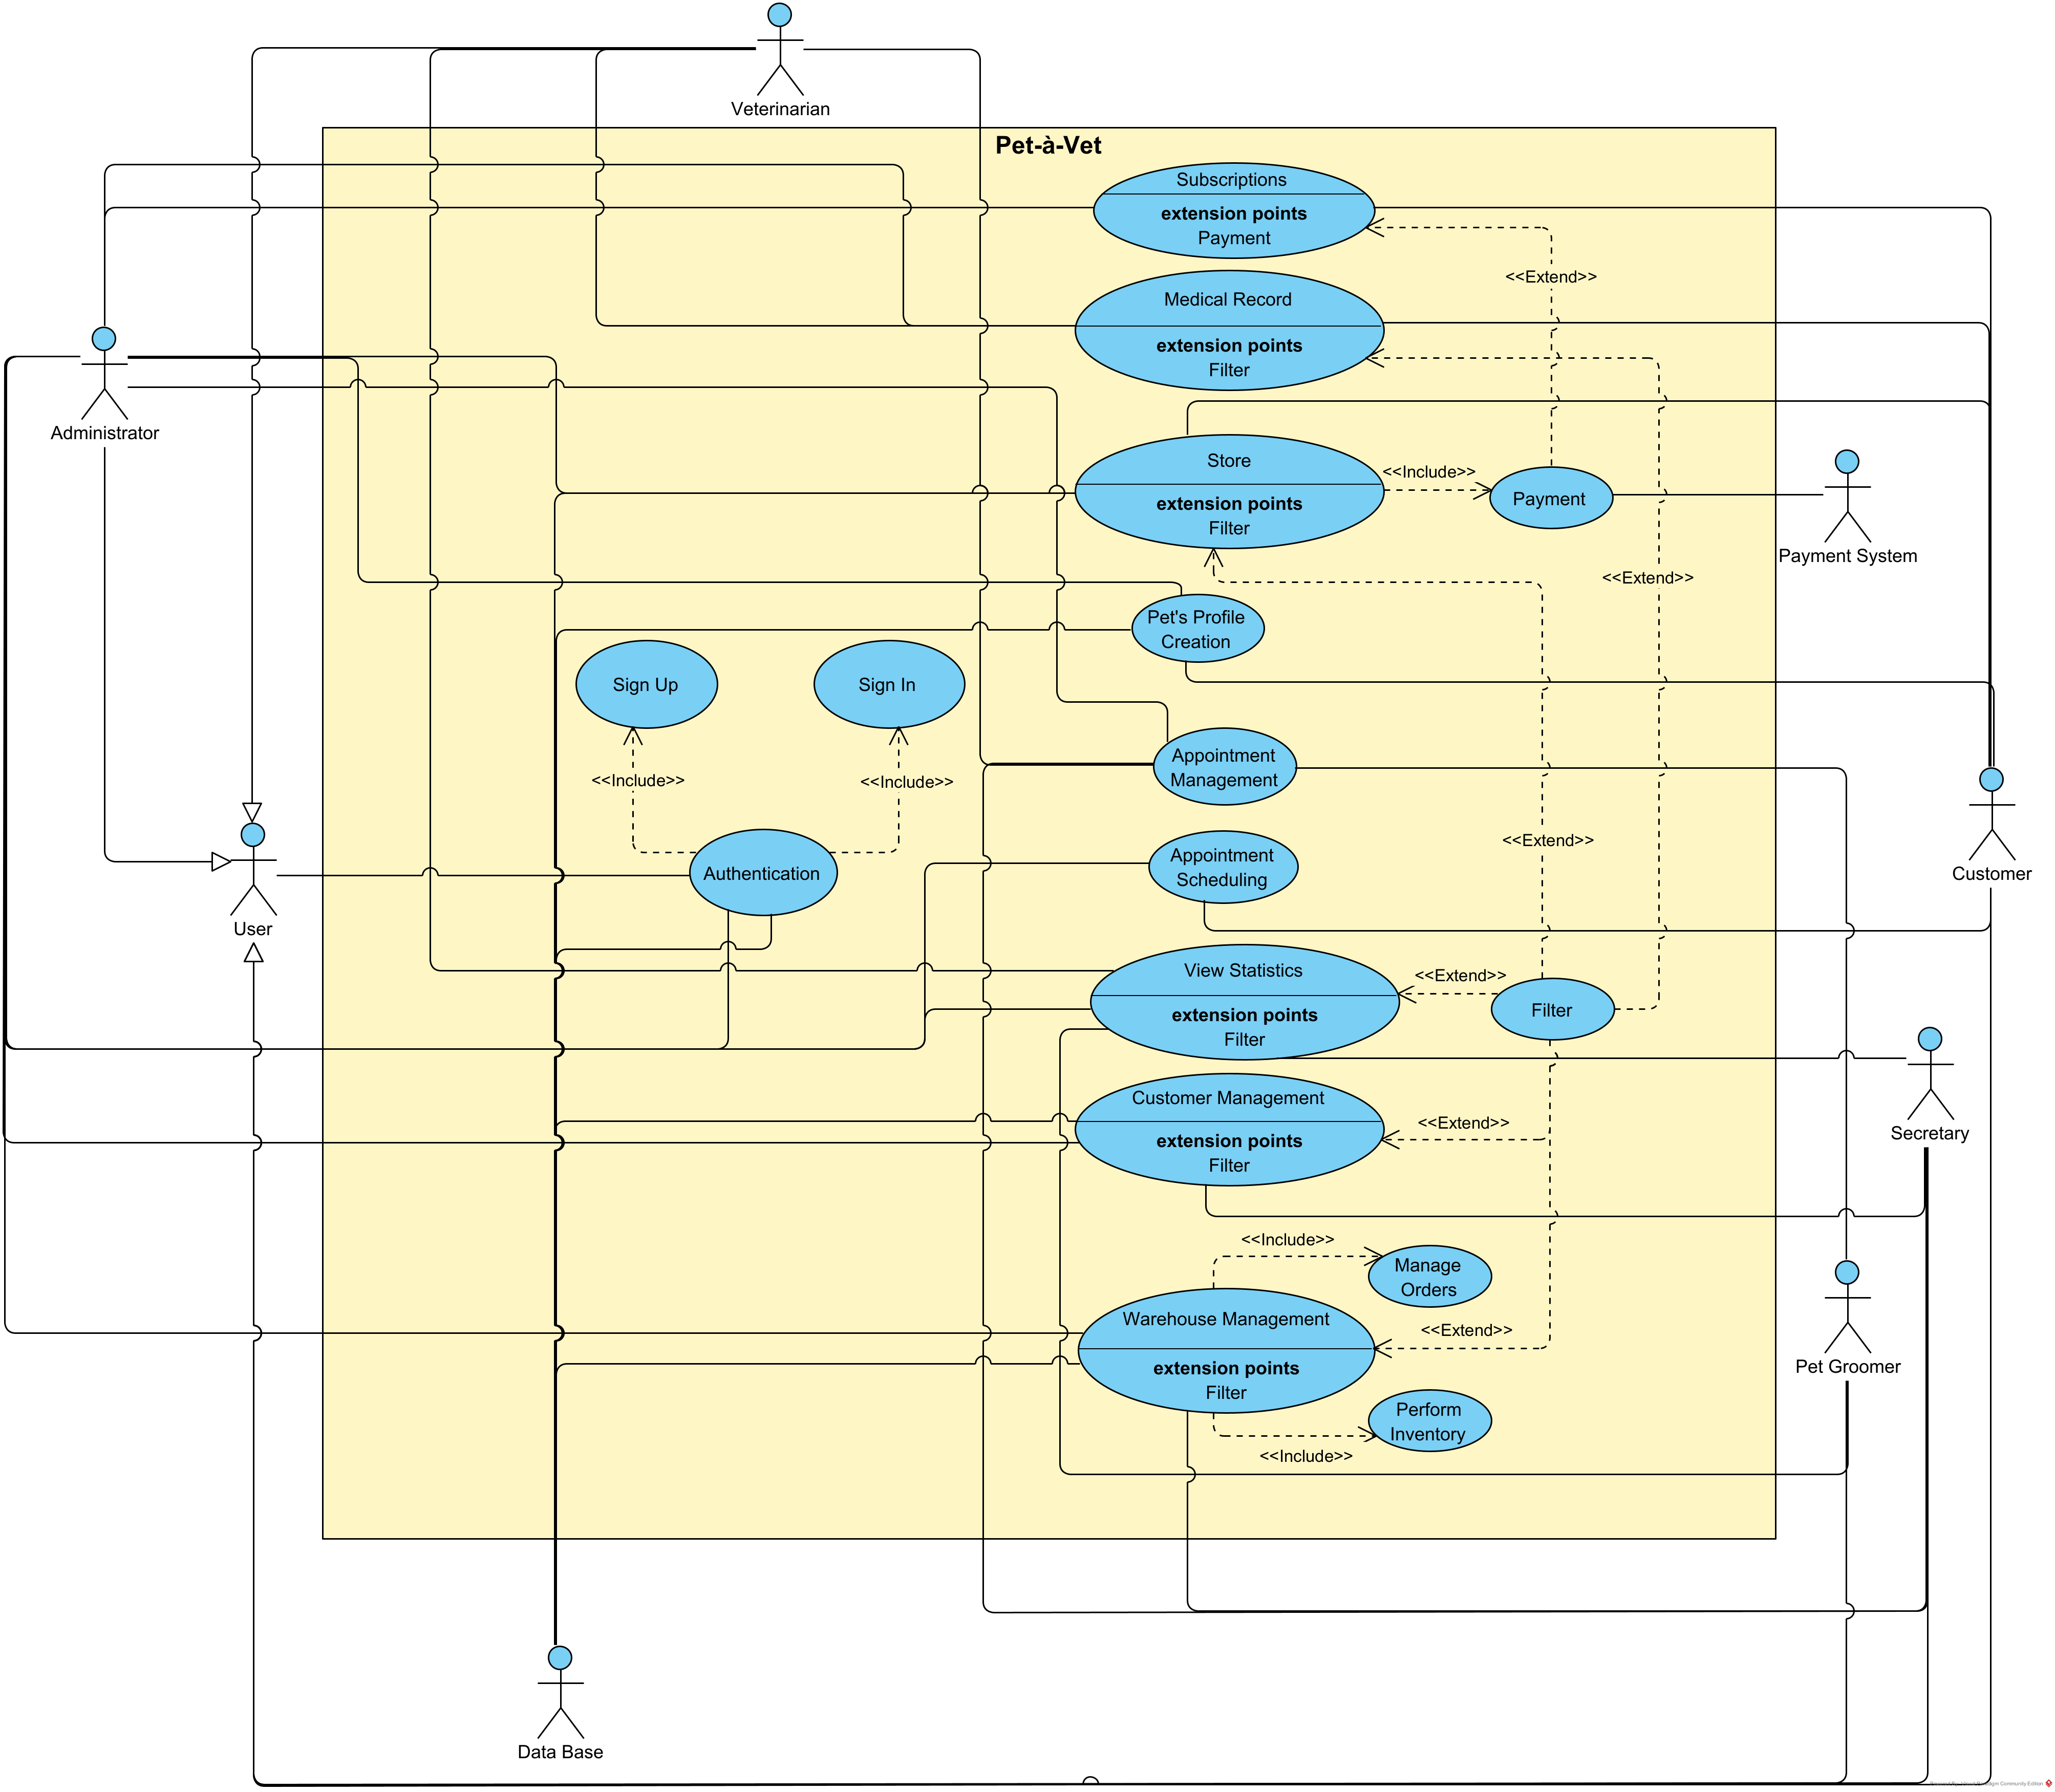
\includegraphics[width=1\textwidth]{Resources/Use-casel-v0.2.png}
  \caption{Διάγραμμα περιπτώσεων χρήσης \textit{Pet-à-Vet}}\label{fig:use-case-diagram}
\end{figure}

\chapter{Domain-model-v0.3}

\section{Εισαγωγή}
Το παρόν κεφάλαιο περιγράφει το Domain Model της εφαρμογής \textit{Pet-à-Vet}. Όλη η ομάδα συναντήθηκε για τη δημιουργία των κλάσεων, των σχέσεων και την περιγραφή τους με τη βοήθεια του εργαλείου \textit{Visual Paradigm}. % chktex 19

Στη τρίτη έκδοση του διαγράμματος, προστέθηκαν περισσότερες κλάσεις, σχέσεις και γνωρίσματα με βάση την ανάπτυξη των διαγραμμάτων ακολουθίας. % chktex 19

\section{Δίαγραμμα}
\begin{figure}[H]
    \centering
    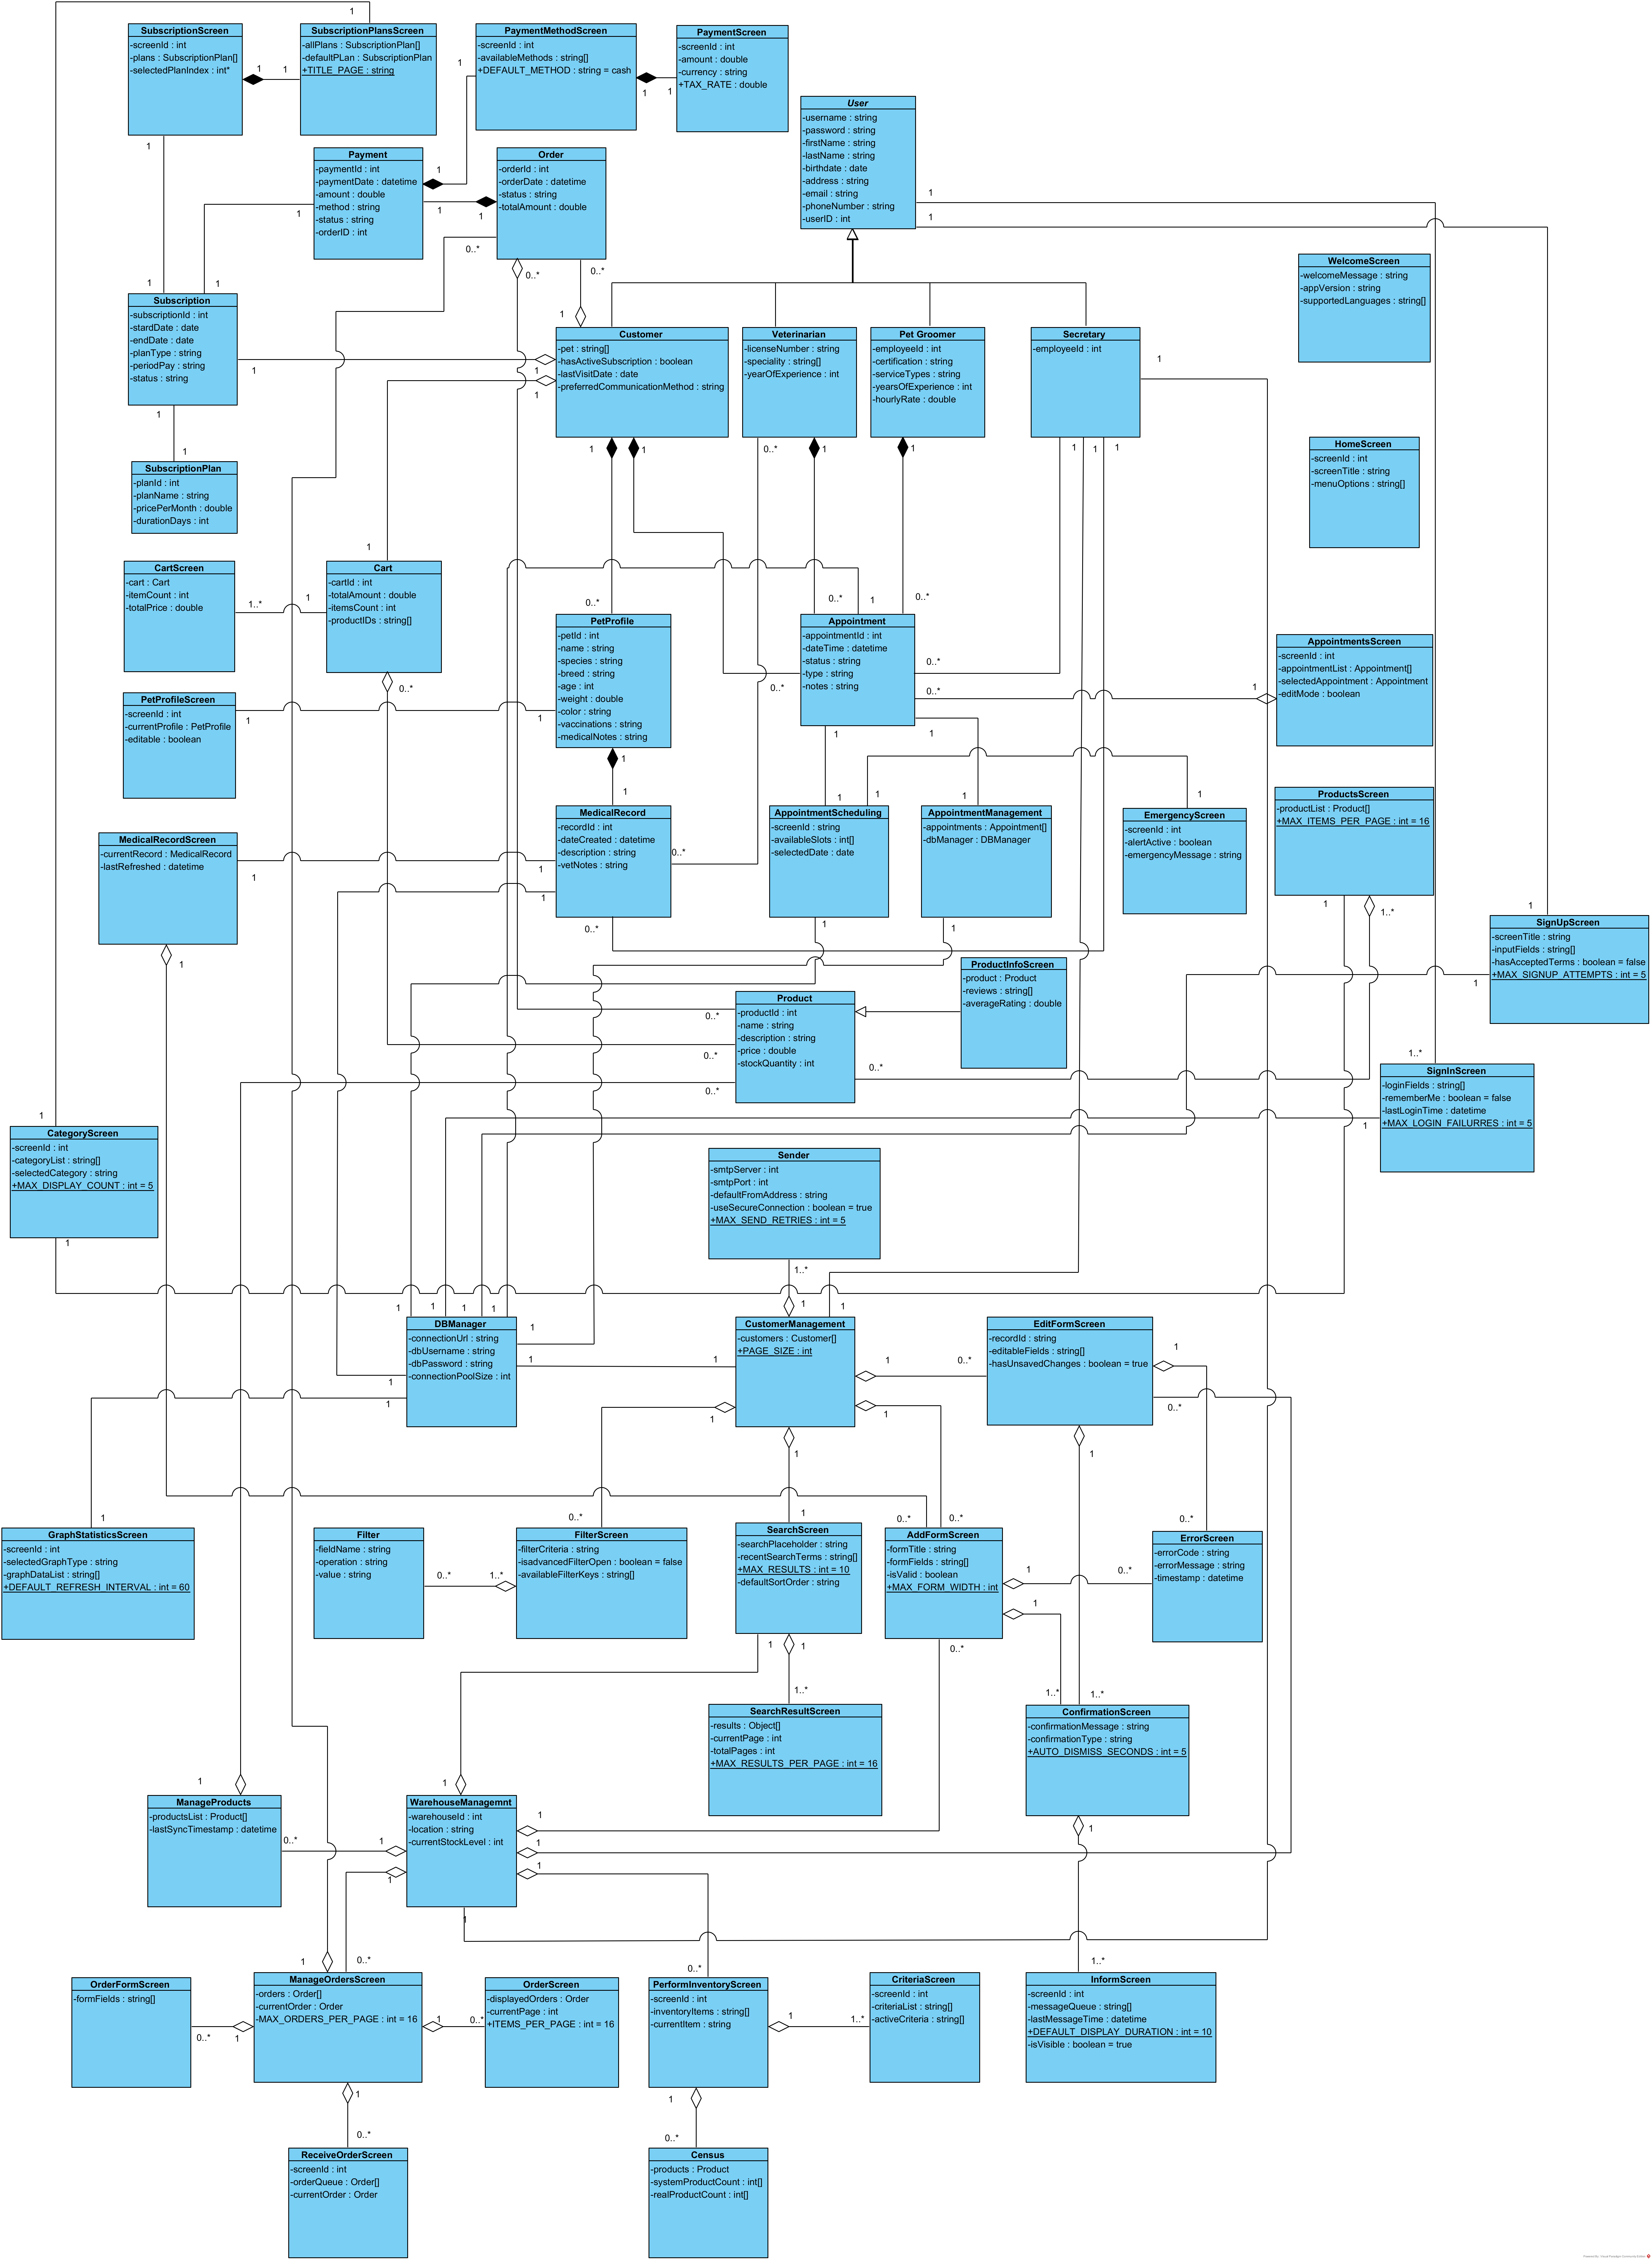
\includegraphics[width=0.63\textwidth]{Resources/Domain-model-v0.2.png}
    \caption{Domain Model του \textit{Pet-à-Vet}}\label{fig:domain_model}
\end{figure}

\section{Περιγραφή}
\begin{itemize}
    \item \textbf{User}\\
          Γενική υπερκλάση από την οποία κληρονομούν οι ρόλοι Customer, Veterinarian, Secretary και Pet Groomer. Περιέχει τα βασικά στοιχεία σύνδεσης και ταυτοποίησης. % chktex 19
    \item \textbf{Customer}\\
          Ο πελάτης του κτηνιατρείου. Μπορεί να καταχωρήσει κατοικίδια, να κλείσει ραντεβού, να διαχειριστεί τις συνδρομές του και να κάνει αγορές προϊόντων. % chktex 19
    \item \textbf{Veterinarian}\\
          Ο γιατρός του κτηνιατρείου. Μπορεί να δει και να ενημερώσει τα ιατρικά αρχεία των κατοικιδίων, να δημιουργεί ραντεβού και να έχει πρόσβαση σε στατιστικά στοιχεία. % chktex 19
    \item \textbf{Secretary}\\
          Ο γραμματέας, που υποστηρίζει τη διαχείριση πελατών, ραντεβού και αποθήκης, καθώς και έχει πρόσβαση στα ιατρικά δεδομένα. % chktex 19
    \item \textbf{PetGroomer}\\
          Ο χρήστης που αναλαμβάνει τις υπηρεσίες καλλωπισμού. Μπορεί να διαχειρίζεται ραντεβού, αλλά δεν έχει πρόσβαση σε ιατρικά αρχεία ή παραγγελίες. % chktex 19
    \item \textbf{PetProfile}\\
          Το κατοικίδιο που ανήκει σε έναν πελάτη. Περιέχει βασικά χαρακτηριστικά (είδος, ηλικία κ.λπ.) και συνδέεται με ιατρικά αρχεία. % chktex 19
    \item \textbf{MedicalRecord}\\
          Περιέχει το ιατρικό ιστορικό του κατοικιδίου. Συνδέεται με τον κτηνίατρο και τα ραντεβού. % chktex 19
    \item \textbf{Appointment}\\
          Ραντεβού που μπορεί να δημιουργηθεί από τον πελάτη, τον γραμματέα ή τον groomer και να αφορά κτηνιατρική επίσκεψη ή καλλωπισμό. % chktex 19
    \item \textbf{Cart}\\
          Το καλάθι αγορών του πελάτη, που περιέχει προϊόντα και οδηγεί σε παραγγελία (Order). % chktex 19
    \item \textbf{Order}\\
          Η παραγγελία που δημιουργείται μετά από αγορά. Συνδέεται με πληρωμή και πελάτη. % chktex 19
    \item \textbf{Payment}\\
          Η πληρωμή για μία παραγγελία ή συνδρομή. Μπορεί να γίνει με κάρτα ή άλλες μεθόδους. % chktex 19
    \item \textbf{Subscription}\\
          Η συνδρομή του πελάτη σε υπηρεσίες με βάση το πακέτο που έχει επιλέξει. Συνδέεται με πληρωμή. % chktex 19
    \item \textbf{Product}\\
          Το προϊόν που ανήκει στην αποθήκη και είναι διαθέσιμο προς πώληση. Περιλαμβάνει ιατροφαρμακευτικά είδη και άλλα προϊόντα. % chktex 19
    \item \textbf{CustomerManagement}\\
          Κλάση για τη διαχείριση πελατών. Παρέχει λειτουργίες για την προσθήκη, επεξεργασία και διαγραφή πελατών, καθώς και την προβολή και αναζήτησή τους. % chktex 19
    \item \textbf{AddFormScreen}\\
          Οθόνη που επιτρέπει την προσθήκη νέων εγγραφών στο σύστημα, όπως πελάτες, κατοικίδια ή προϊόντα. Διαχειρίζεται τα πεδία εισαγωγής και την επικύρωση των δεδομένων. % chktex 19
    \item \textbf{ConfirmationScreen}\\
          Οθόνη που εμφανίζει μηνύματα επιβεβαίωσης μετά από επιτυχείς ενέργειες, όπως ολοκλήρωση πληρωμής ή καταχώρηση ραντεβού.
    \item \textbf{DBManager}\\
          Διαχειρίζεται τη σύνδεση και την επικοινωνία με τη βάση δεδομένων. Παρέχει μεθόδους για την ανάκτηση και αποθήκευση δεδομένων. % chktex 19
    \item \textbf{Sender}\\
          Υπεύθυνη για την αποστολή ειδοποιήσεων, emails και SMS στους χρήστες, όπως υπενθυμίσεις ραντεβού, επιβεβαιώσεις παραγγελιών κ.λπ. % chktex 19
    \item \textbf{SearchScreen}\\
          Οθόνη αναζήτησης που επιτρέπει στους χρήστες να βρίσκουν πελάτες, κατοικίδια, προϊόντα ή ραντεβού με βάση συγκεκριμένα κριτήρια. % chktex 19
    \item \textbf{SearchResultScreen}\\
          Οθόνη που εμφανίζει τα αποτελέσματα μιας αναζήτησης και επιτρέπει την περαιτέρω αλληλεπίδραση με αυτά. % chktex 19
    \item \textbf{EditFormScreen}\\
          Οθόνη που επιτρέπει την επεξεργασία υπαρχόντων εγγραφών στο σύστημα.
    \item \textbf{ErrorScreen}\\
          Οθόνη που εμφανίζεται σε περίπτωση σφάλματος, παρέχοντας πληροφορίες για το πρόβλημα και πιθανές λύσεις.
    \item \textbf{FilterScreen}\\
          Οθόνη που επιτρέπει το φιλτράρισμα δεδομένων με βάση διάφορα κριτήρια. Συνεργάζεται με την κλάση Filter. % chktex 19
    \item \textbf{Filter}\\
          Κλάση που υλοποιεί τη λογική φιλτραρίσματος δεδομένων με βάση κριτήρια που ορίζει ο χρήστης. % chktex 19
    \item \textbf{WarehouseManagemnt}\\
          Κλάση για τη διαχείριση της αποθήκης, συμπεριλαμβανομένης της παρακολούθησης αποθέματος, των παραγγελιών και των ημερομηνιών λήξης. % chktex 19
    \item \textbf{ManageProducts}\\
          Παρέχει λειτουργίες για τη διαχείριση των προϊόντων που διατίθενται από το κτηνιατρείο, όπως προσθήκη, τροποποίηση και διαγραφή. % chktex 19
    \item \textbf{InformScreen}\\
          Οθόνη που εμφανίζει ενημερωτικά μηνύματα και πληροφορίες για τους χρήστες.
    \item \textbf{PerformInventoryScreen}\\
          Οθόνη για την εκτέλεση απογραφής στην αποθήκη, επιτρέποντας την καταμέτρηση και την καταγραφή του τρέχοντος αποθέματος.
    \item \textbf{Census}\\
          Κλάση που χρησιμοποιείται για την απογραφή προϊόντων της αποθήκης. % chktex 19
    \item \textbf{CriteriaScreen}\\
          Οθόνη που επιτρέπει τον καθορισμό κριτηρίων για διάφορες λειτουργίες, όπως αναζήτηση ή δημιουργία αναφορών. % chktex 19
    \item \textbf{ManageOrdersScreen}\\
          Οθόνη για τη διαχείριση παραγγελιών, συμπεριλαμβανομένης της προβολής, επεξεργασίας και καταγραφής νέων παραγγελιών. % chktex 19
    \item \textbf{OrderFormScreen}\\
          Φόρμα για τη δημιουργία ή επεξεργασία μιας παραγγελίας. % chktex 19
    \item \textbf{OrderScreen}\\
          Κύρια οθόνη διαχείρισης και προβολής παραγγελιών. % chktex 19
    \item \textbf{ReceiveOrderScreen}\\
          Οθόνη για την καταγραφή της παραλαβής παραγγελιών και την ενημέρωση του αποθέματος.
    \item \textbf{HomeScreen}\\
          Η κεντρική οθόνη της εφαρμογής, που παρέχει πρόσβαση σε όλες τις κύριες λειτουργίες.
    \item \textbf{CategoryScreen}\\
          Οθόνη που εμφανίζει κατηγορίες προϊόντων ή υπηρεσιών.
    \item \textbf{GraphStatisticsScreen}\\
          Οθόνη που παρουσιάζει στατιστικά δεδομένα με τη μορφή γραφημάτων για την υποστήριξη αποφάσεων. % chktex 19
    \item \textbf{AppointmentsScreen}\\
          Οθόνη που εμφανίζει όλα τα προγραμματισμένα ραντεβού και επιτρέπει την αλληλεπίδραση με αυτά. % chktex 19
    \item \textbf{MedicalRecordScreen}\\
          Οθόνη προβολής και επεξεργασίας ιατρικών αρχείων των κατοικίδιων. % chktex 19
    \item \textbf{SubscriptionScreen}\\
          Οθόνη διαχείρισης συνδρομών που επιτρέπει την προβολή, αγορά ή ανανέωσή τους. % chktex 19
    \item \textbf{SubscriptionPlansScreen}\\
          Οθόνη που εμφανίζει τα διαθέσιμα πακέτα συνδρομών και τα χαρακτηριστικά τους. % chktex 19
    \item \textbf{AppointmentManagement}\\
          Κλάση για τη διαχείριση των ραντεβού από την πλευρά των επαγγελματιών (κτηνίατροι, groomer, γραμματείς). % chktex 19
    \item \textbf{AppointmentScheduling}\\
          Κλάση για τον προγραμματισμό νέων ραντεβού από την πλευρά των πελατών.
    \item \textbf{WelcomeScreen}\\
          Η αρχική οθόνη που βλέπει ο χρήστης όταν ανοίγει την εφαρμογή για πρώτη φορά.
    \item \textbf{SignUpScreen}\\
          Οθόνη εγγραφής νέου χρήστη στην εφαρμογή.
    \item \textbf{SignInScreen}\\
          Οθόνη σύνδεσης υπάρχοντος χρήστη. % chktex 19
    \item \textbf{ProductsScreen}\\
          Οθόνη προβολής και αναζήτησης προϊόντων προς αγορά.
    \item \textbf{CartScreen}\\
          Οθόνη που εμφανίζει τα προϊόντα στο καλάθι του χρήστη και επιτρέπει την ολοκλήρωση της αγοράς.
    \item \textbf{ProductInfoScreen}\\
          Οθόνη με λεπτομερείς πληροφορίες για ένα συγκεκριμένο προϊόν.
    \item \textbf{PaymentMethodScreen}\\
          Οθόνη επιλογής μεθόδου πληρωμής κατά τη διαδικασία ολοκλήρωσης μιας αγοράς. % chktex 19
    \item \textbf{PaymentScreen}\\
          Οθόνη ολοκλήρωσης πληρωμής.
    \item \textbf{EmergencyScreen}\\
          Οθόνη για την καταγραφή και διαχείριση επειγόντων περιστατικών που απαιτούν άμεση προσοχή. % chktex 19
    \item \textbf{PetProfileScreen}\\
          Οθόνη προβολής και επεξεργασίας του προφίλ ενός κατοικίδιου. % chktex 19
    \item \textbf{SubscriptionPlan}\\
          Κλάση που περιγράφει ένα συγκεκριμένο πακέτο συνδρομής, με τα χαρακτηριστικά και την τιμή του. % chktex 19
\end{itemize}

\chapter{Αναφορές}

Σύνδεσμοι για την αναφορά των διαγραμμάτων: % chktex 19
\begin{itemize}
    \item \href{https://www.visual-paradigm.com/}{Visual Paradigm}
    \item \href{https://www.latex-project.org/}{LaTeX}
\end{itemize}

Η ομάδα του \textit{Pet-à-Vet} βασίστηκε στο διαθέσιμο υλικό που παρέχεται στη ηλεκτρονική πλατφόρμα του μαθήματος \href{https://eclass.upatras.gr/courses/CEID1030/}{\textit{Τεχνολογία Λογισμικού}}. % chktex 19

\end{document} % chktex 17